% Options for packages loaded elsewhere
\PassOptionsToPackage{unicode}{hyperref}
\PassOptionsToPackage{hyphens}{url}
%
\documentclass[
]{book}
\usepackage{amsmath,amssymb}
\usepackage{lmodern}
\usepackage{ifxetex,ifluatex}
\ifnum 0\ifxetex 1\fi\ifluatex 1\fi=0 % if pdftex
  \usepackage[T1]{fontenc}
  \usepackage[utf8]{inputenc}
  \usepackage{textcomp} % provide euro and other symbols
\else % if luatex or xetex
  \usepackage{unicode-math}
  \defaultfontfeatures{Scale=MatchLowercase}
  \defaultfontfeatures[\rmfamily]{Ligatures=TeX,Scale=1}
\fi
% Use upquote if available, for straight quotes in verbatim environments
\IfFileExists{upquote.sty}{\usepackage{upquote}}{}
\IfFileExists{microtype.sty}{% use microtype if available
  \usepackage[]{microtype}
  \UseMicrotypeSet[protrusion]{basicmath} % disable protrusion for tt fonts
}{}
\makeatletter
\@ifundefined{KOMAClassName}{% if non-KOMA class
  \IfFileExists{parskip.sty}{%
    \usepackage{parskip}
  }{% else
    \setlength{\parindent}{0pt}
    \setlength{\parskip}{6pt plus 2pt minus 1pt}}
}{% if KOMA class
  \KOMAoptions{parskip=half}}
\makeatother
\usepackage{xcolor}
\IfFileExists{xurl.sty}{\usepackage{xurl}}{} % add URL line breaks if available
\IfFileExists{bookmark.sty}{\usepackage{bookmark}}{\usepackage{hyperref}}
\hypersetup{
  pdftitle={R Eğitim},
  pdfauthor={Melike Dönertaş},
  hidelinks,
  pdfcreator={LaTeX via pandoc}}
\urlstyle{same} % disable monospaced font for URLs
\usepackage{color}
\usepackage{fancyvrb}
\newcommand{\VerbBar}{|}
\newcommand{\VERB}{\Verb[commandchars=\\\{\}]}
\DefineVerbatimEnvironment{Highlighting}{Verbatim}{commandchars=\\\{\}}
% Add ',fontsize=\small' for more characters per line
\usepackage{framed}
\definecolor{shadecolor}{RGB}{248,248,248}
\newenvironment{Shaded}{\begin{snugshade}}{\end{snugshade}}
\newcommand{\AlertTok}[1]{\textcolor[rgb]{0.94,0.16,0.16}{#1}}
\newcommand{\AnnotationTok}[1]{\textcolor[rgb]{0.56,0.35,0.01}{\textbf{\textit{#1}}}}
\newcommand{\AttributeTok}[1]{\textcolor[rgb]{0.77,0.63,0.00}{#1}}
\newcommand{\BaseNTok}[1]{\textcolor[rgb]{0.00,0.00,0.81}{#1}}
\newcommand{\BuiltInTok}[1]{#1}
\newcommand{\CharTok}[1]{\textcolor[rgb]{0.31,0.60,0.02}{#1}}
\newcommand{\CommentTok}[1]{\textcolor[rgb]{0.56,0.35,0.01}{\textit{#1}}}
\newcommand{\CommentVarTok}[1]{\textcolor[rgb]{0.56,0.35,0.01}{\textbf{\textit{#1}}}}
\newcommand{\ConstantTok}[1]{\textcolor[rgb]{0.00,0.00,0.00}{#1}}
\newcommand{\ControlFlowTok}[1]{\textcolor[rgb]{0.13,0.29,0.53}{\textbf{#1}}}
\newcommand{\DataTypeTok}[1]{\textcolor[rgb]{0.13,0.29,0.53}{#1}}
\newcommand{\DecValTok}[1]{\textcolor[rgb]{0.00,0.00,0.81}{#1}}
\newcommand{\DocumentationTok}[1]{\textcolor[rgb]{0.56,0.35,0.01}{\textbf{\textit{#1}}}}
\newcommand{\ErrorTok}[1]{\textcolor[rgb]{0.64,0.00,0.00}{\textbf{#1}}}
\newcommand{\ExtensionTok}[1]{#1}
\newcommand{\FloatTok}[1]{\textcolor[rgb]{0.00,0.00,0.81}{#1}}
\newcommand{\FunctionTok}[1]{\textcolor[rgb]{0.00,0.00,0.00}{#1}}
\newcommand{\ImportTok}[1]{#1}
\newcommand{\InformationTok}[1]{\textcolor[rgb]{0.56,0.35,0.01}{\textbf{\textit{#1}}}}
\newcommand{\KeywordTok}[1]{\textcolor[rgb]{0.13,0.29,0.53}{\textbf{#1}}}
\newcommand{\NormalTok}[1]{#1}
\newcommand{\OperatorTok}[1]{\textcolor[rgb]{0.81,0.36,0.00}{\textbf{#1}}}
\newcommand{\OtherTok}[1]{\textcolor[rgb]{0.56,0.35,0.01}{#1}}
\newcommand{\PreprocessorTok}[1]{\textcolor[rgb]{0.56,0.35,0.01}{\textit{#1}}}
\newcommand{\RegionMarkerTok}[1]{#1}
\newcommand{\SpecialCharTok}[1]{\textcolor[rgb]{0.00,0.00,0.00}{#1}}
\newcommand{\SpecialStringTok}[1]{\textcolor[rgb]{0.31,0.60,0.02}{#1}}
\newcommand{\StringTok}[1]{\textcolor[rgb]{0.31,0.60,0.02}{#1}}
\newcommand{\VariableTok}[1]{\textcolor[rgb]{0.00,0.00,0.00}{#1}}
\newcommand{\VerbatimStringTok}[1]{\textcolor[rgb]{0.31,0.60,0.02}{#1}}
\newcommand{\WarningTok}[1]{\textcolor[rgb]{0.56,0.35,0.01}{\textbf{\textit{#1}}}}
\usepackage{longtable,booktabs,array}
\usepackage{calc} % for calculating minipage widths
% Correct order of tables after \paragraph or \subparagraph
\usepackage{etoolbox}
\makeatletter
\patchcmd\longtable{\par}{\if@noskipsec\mbox{}\fi\par}{}{}
\makeatother
% Allow footnotes in longtable head/foot
\IfFileExists{footnotehyper.sty}{\usepackage{footnotehyper}}{\usepackage{footnote}}
\makesavenoteenv{longtable}
\usepackage{graphicx}
\makeatletter
\def\maxwidth{\ifdim\Gin@nat@width>\linewidth\linewidth\else\Gin@nat@width\fi}
\def\maxheight{\ifdim\Gin@nat@height>\textheight\textheight\else\Gin@nat@height\fi}
\makeatother
% Scale images if necessary, so that they will not overflow the page
% margins by default, and it is still possible to overwrite the defaults
% using explicit options in \includegraphics[width, height, ...]{}
\setkeys{Gin}{width=\maxwidth,height=\maxheight,keepaspectratio}
% Set default figure placement to htbp
\makeatletter
\def\fps@figure{htbp}
\makeatother
\setlength{\emergencystretch}{3em} % prevent overfull lines
\providecommand{\tightlist}{%
  \setlength{\itemsep}{0pt}\setlength{\parskip}{0pt}}
\setcounter{secnumdepth}{5}
\usepackage{booktabs}
\ifluatex
  \usepackage{selnolig}  % disable illegal ligatures
\fi
\usepackage[]{natbib}
\bibliographystyle{apalike}

\title{R Eğitim}
\author{Melike Dönertaş}
\date{22-03-2021}

\begin{document}
\maketitle

{
\setcounter{tocdepth}{1}
\tableofcontents
}
\hypertarget{bilgilendirme}{%
\chapter*{Bilgilendirme}\label{bilgilendirme}}
\addcontentsline{toc}{chapter}{Bilgilendirme}

22 Mart 2021 tarihinde Bioinforange tarafından düzenlenen Bioinfoconference kapsamında verilen R Eğitim çalıştay materyalini içerir. Çalıştay materyali Melike Dönertaş tarafından hazırlanmıştır, öneri ve düzeltmeler için konu başlığında ``{[}Bioinforange R Eğitim{]}'' kullanarak \href{mailto:donertas.melike@gmail.com}{email} ile ulaşabilirsiniz.

\hypertarget{yardux131m}{%
\section*{Yardım}\label{yardux131m}}
\addcontentsline{toc}{section}{Yardım}

R konusunda karşılaştığınız sorular için öncelikle aldığınız hata ve uyarıları incelemenizi, \texttt{?} operatörünü veya \texttt{help()} komutunu kullanarak fonksiyon, veriseti ve obje yardım sayfalarına bakmanızı, R sıkça sorulan sorular kitapçıklarına sorularınızın dahil olup olmadığını kontrol etmenizi (\href{https://cran.r-project.org/doc/FAQ/R-FAQ.html}{Genel SSS}, \href{https://cran.r-project.org/bin/windows/base/rw-FAQ.html}{Windows'a özgü SSS}, \href{https://cran.r-project.org/bin/macosx/RMacOSX-FAQ.html}{Mac OS'a özgü SSS}), bir paket kullanıyorsanız ve sorunuz bununla ilgiliyse paket yardım ve kullanım örnekleri dosyalarını incelemenizi, ve eğer bu aşamalardan sonra hala cevap bulamadıysanız sorunuzu ``\href{https://stackoverflow.com/help/how-to-ask}{Nasıl güzel soru sorulur?}'' yönergesine göz attıktan sonra \href{https://stackoverflow.com/questions/tagged/r}{Stack Overflow R bölümü}ne sormanızı tavsiye ederim. Alternatif olarak, kodlama konusunda yardımlaşma platformlarına (\href{https://rsgturkey.com/}{RSG Türkiye}'nin Slack kanalı gibi\footnote{bu şekilde başka platformlar biliyorsanız lütfen bildirin, güncelleyebilirim}) sorularınızı gönderebilirsiniz.

\hypertarget{uxe7alux131ux15ftay-iuxe7eriux11fi}{%
\chapter{Çalıştay içeriği}\label{uxe7alux131ux15ftay-iuxe7eriux11fi}}

R'a giriş niteliğinde birkaç ders içeriği zaten mevcut. Bu çalıştayda, süremizin sadece 2 saat olduğunu ve interaktifliğin kısıtlı olduğunu göz önüne alarak, bir R eğitiminden ziyade R'ın biyolojide uygulamalarına yönelik kısa bir örnekleme hedefledim. Çalıştay R'daki temel işlemler, operatörler, fonksiyonlar ve görselleştirme araçlarının kullanımına örnekler içerecek. Bunun için bir transkriptom veriseti kullanacağız. Bu veriseti halka açık veritabanı olan GEO'dan indirilecek. Ancak bu çalıştay ``transkriptom veri analizi nasıl yapılır?''ı öğretmeyi amaçlamamaktadır. Transkriptom veri analizinde batch etkileri, normalizasyon gereklilikleri vs.~bir çok kaygı vardır ve buna göre analiz basamakları gerektirmektedir. Burada yapacağımız örnek çok basit olup, gerekli olabilecek bazı basamakları atlamaktadır, bu sebeple transkriptom veri analizi örneği olarak değil R uygulamasına örnek olarak düşünülmelidir.

\hypertarget{giriux15f}{%
\chapter{Giriş}\label{giriux15f}}

\hypertarget{r-kurulumu}{%
\section{R Kurulumu}\label{r-kurulumu}}

R'ı kullandığınız işletim sistemine göre \href{https://cran.r-project.org/}{CRAN anasayfası}ndan indirebilirsiniz. Özellikle başlangıç seviyesinde \texttt{base} indirmek yeterli olacaktır. Kaynak kodu R bazlı değil de C/C++/Fortran gibi dillerde yazılmış olan paketleri kurmak için \texttt{Rtools} indirmeniz gerekebilir ama şimdilik \texttt{base} indirerek devam edebiliriz.

\hypertarget{rstudio}{%
\section{RStudio}\label{rstudio}}

RStudio, R için bir IDE yani ``entegre geliştirme ortamı''dır ve ücretsiz olarak \href{https://www.rstudio.com/}{RStudio websayfası}ndan indirilebilir. Entegre geliştirme ortamları kod yazma, sonuçları ve çizdiğiniz grafikleri vs.~görüntüleme, otomasyon, hata ayıklama (debugging) gibi programlama ve yazılım geliştirme bileşenlerini içinde bulunduran araçlardır. RStudio ise bunların ötesinde başka programlama dilleriyle beraber kodlama, raporlama, versiyon kontrolü, komut istemcisi ve zamanlı iş çalıştırma ve daha bir çok özellik ile birlikte geliyor. R kodlama için kesinlikle RStudio ile çalışılmasını öneriyorum.

\hypertarget{baux15flangux131uxe7}{%
\section{Başlangıç}\label{baux15flangux131uxe7}}

Hem R hem Rstudio'yu yükleyip, RStudio açtığımızda karşımıza 3 ekran çıkar. Bunlar haricinde sol üst köşedeki ``yeni'' tuşuna basıp R Scriptini seçersek 4. ekran açılır. Hızlıca bunların içeriğine bakalım:

\begin{itemize}
\tightlist
\item
  Files: İçinde bulunduğumuz klasörün içindeki dosyaları listeliyor.
\item
  Console: Burası kodu yazıp sonuçları gördüğümüz kısım. Denemek için \texttt{2+2} yazıp enter'a basalım.
\item
  Terminal: Burası da bilgisayarınızın terminali veya komut istemcisine erişim sağlayan bir kısım.
\item
  Environment: Oluşturduğumuz değişkenlerin listesini ve bilgilerini burada görebiliriz.
\item
  Plots: Çizdiğimiz grafikleri görüntüleyebileceğimiz kısım.
\item
  Help: Bu sekme RStudio'daki en büyük dostumuz. Açıp öğrenme linklerini kurcalamak iyi bir başlangıç. Ayrıca \texttt{?} operatörü ile burada fonksiyonların yardım sayfalarını görüntüleyebiliriz.
\item
  History: Mevcut R oturumunuzda yazdığınız kodları listeleyen bir kısım. Buradan önceden çalıştırdığınız kodları görebilirsiniz. Ancak daha pratik, daha çok kullanılan bir kısa yol, konsolda iken klavyedeki yukarı ok tuşu ile önceki kodları tekrar çağırmak. Geçmiş sadece açık oturumdaki kodları kaydediyor olsa da, .Rhistory dosyası sayesinde ortamlar arası geçmiş bilgisini aktarabilirsiniz. Yine de buna bağlı kalmak yerine daha sonra tekrar kullanacağımız kodları .R scripti olarak kaydetmek çok daha elverişli olacaktır.
\item
  Packages: R'da yüklü olan çeşitli paketleri (kütüphaneleri) görüyoruz. Ancak buradan R ortamımıza yükleme yapmaktansa \texttt{library()} komutunu kullanmalıyız ki yazdığımız kodlar daha sonra hem biz hem başkaları tarafından kolaylıkla çalıştırılabilsin.
\end{itemize}

Bunlardan yeni açtığımız ekran da script (betik) editör ekranı, yani kodu yazıp kaydedeceğimiz kod editörümüz. Kodu konsola yazıp çalıştabiliriz ama önerim hep editörde çalışıp çalışan kodları kaydetmeniz. Editörde yazdığımız kodu kopyala yapıştır yapmadan çalıştırmanın kolay bir yolu var: Windows'ta Ctrl + Enter, Mac'te Cmd + Enter.

\hypertarget{temel-bilgiler}{%
\chapter{Temel Bilgiler}\label{temel-bilgiler}}

Kodlari editorde yazip Ctrl+Enter ile calistirabilirsiniz. Alternatif olarak Konsol'da da kodlari yazabilirsiniz ancak editore yazdiklarinizi kaydederek yazdiklarinizdan elinizde bulunmasini istediklerinizi kaydedebilirsiniz. Onerim hep konsolu kullanmaniz, kullanisli olan kodlari tutup digerlerini / calismayanlari silip temiz bir sekilde dosyanizi kaydetmeniz.

Ilk olarak hangi klasorde nerde calisiyoruz buna bakalim. Bu R'da dosya acarken ve yaptiklarimizi kaydederken onemli bir detay. Bunun icin \texttt{getwd()} yani `get directory' komutunu kullanacagiz. Bunu calistirdigimizda aldigimiz sonuc hepimizde farkli olacaktir. Bu bilgisayarinizda nerede calistiginizi gosteriyor:

\begin{Shaded}
\begin{Highlighting}[]
\FunctionTok{getwd}\NormalTok{()}
\end{Highlighting}
\end{Shaded}

\begin{verbatim}
## [1] "/Users/melike/GDrive/githubbooks/20210322_REgitim"
\end{verbatim}

Bu varsayilan ortamda degil de belli bir klasorun icinde calismak istiyorsaniz, istediginiz klasore \texttt{setwd()} fonksiyonu ile asagidaki sekilde gecebiliriz. Ancak onerim az sonra aciklayacagim sekilde RStudio projesi kullanmaniz.

\begin{Shaded}
\begin{Highlighting}[]
\FunctionTok{setwd}\NormalTok{(}\StringTok{"\textasciitilde{}/GDrive/projects/R\_Egitim"}\NormalTok{)}
\end{Highlighting}
\end{Shaded}

\hypertarget{rstudio-projesi}{%
\section{RStudio projesi}\label{rstudio-projesi}}

R'da calisirken her zaman proje olusturmanizi tavsiye ederim. Bu sayede hem her projenize ait kod tarihi ayrica saklanir, hem de calistiginiz klasor vs.~gibi konularda endiselenmeniz gerekmez. RStudio projelerinin bunlar haricinde versiyon kontrol konusu vs.~gibi ileri asamalarda kullanacaginiz diger konularda da fayda saglar. Sag ust kosedeki New Project'e basip, 'yeni klasor'u secerek yeni proje olusturabilirsiniz. Bunu yaptiktan sonra \texttt{getwd()} fonksiyonunu tekrar calistiralim:

\begin{Shaded}
\begin{Highlighting}[]
\FunctionTok{getwd}\NormalTok{()}
\end{Highlighting}
\end{Shaded}

\begin{verbatim}
## [1] "/Users/melike/GDrive/githubbooks/20210322_REgitim"
\end{verbatim}

Benim sonucumda degisen bir sey yok cunku zaten proje icinde calisiyordum ancak sizin sonucunuz degismis olmali.

\hypertarget{hesap-makinesi-olarak-r}{%
\section{Hesap makinesi olarak R}\label{hesap-makinesi-olarak-r}}

\begin{Shaded}
\begin{Highlighting}[]
\DecValTok{2}\SpecialCharTok{+}\DecValTok{2}
\end{Highlighting}
\end{Shaded}

\begin{verbatim}
## [1] 4
\end{verbatim}

\begin{Shaded}
\begin{Highlighting}[]
\DecValTok{5}\SpecialCharTok{*}\DecValTok{7}
\end{Highlighting}
\end{Shaded}

\begin{verbatim}
## [1] 35
\end{verbatim}

\begin{Shaded}
\begin{Highlighting}[]
\DecValTok{20{-}4}
\end{Highlighting}
\end{Shaded}

\begin{verbatim}
## [1] 16
\end{verbatim}

\begin{Shaded}
\begin{Highlighting}[]
\DecValTok{3}\SpecialCharTok{\^{}}\DecValTok{2}
\end{Highlighting}
\end{Shaded}

\begin{verbatim}
## [1] 9
\end{verbatim}

\begin{Shaded}
\begin{Highlighting}[]
\DecValTok{100}\SpecialCharTok{/}\DecValTok{2}
\end{Highlighting}
\end{Shaded}

\begin{verbatim}
## [1] 50
\end{verbatim}

\begin{Shaded}
\begin{Highlighting}[]
\DecValTok{9}\SpecialCharTok{\%\%}\DecValTok{5}
\end{Highlighting}
\end{Shaded}

\begin{verbatim}
## [1] 4
\end{verbatim}

\begin{Shaded}
\begin{Highlighting}[]
\DecValTok{9}\SpecialCharTok{\%/\%}\DecValTok{5}
\end{Highlighting}
\end{Shaded}

\begin{verbatim}
## [1] 1
\end{verbatim}

\hypertarget{fonksiyonlar}{%
\section{Fonksiyonlar}\label{fonksiyonlar}}

R kendi yazacaginiz fonksiyonlarin yaninda kendi icinde cok sayida fonksiyon barindirir, az once kullandigimiz \texttt{getwd()} fonksiyonu gibi. Bunlar fonksiyon adini takiben, parantez icinde belli argumanlar alirlar. Birkac ornek:

\begin{Shaded}
\begin{Highlighting}[]
\FunctionTok{log10}\NormalTok{(}\AttributeTok{x =} \DecValTok{100}\NormalTok{)}
\end{Highlighting}
\end{Shaded}

\begin{verbatim}
## [1] 2
\end{verbatim}

\begin{Shaded}
\begin{Highlighting}[]
\FunctionTok{log10}\NormalTok{(}\DecValTok{100}\NormalTok{)}
\end{Highlighting}
\end{Shaded}

\begin{verbatim}
## [1] 2
\end{verbatim}

\begin{Shaded}
\begin{Highlighting}[]
\FunctionTok{sqrt}\NormalTok{(}\DecValTok{16}\NormalTok{)}
\end{Highlighting}
\end{Shaded}

\begin{verbatim}
## [1] 4
\end{verbatim}

\hypertarget{yardux131m-almak}{%
\subsection{Yardım almak}\label{yardux131m-almak}}

R'da cogu fonksiyon yardim sayfasi icerir ve bunlara \texttt{?} operatoru ile ulasilir:

\begin{Shaded}
\begin{Highlighting}[]
\NormalTok{?log10}
\NormalTok{?getwd}
\end{Highlighting}
\end{Shaded}

\hypertarget{deux11fiux15fkenlerle-uxe7alux131ux15fmak}{%
\section{Değişkenlerle çalışmak}\label{deux11fiux15fkenlerle-uxe7alux131ux15fmak}}

Degiskenler veri tutuculardir. Degisken atamak icin \texttt{\textless{}-} ya da \texttt{=} operatorleri kullanilir. Tarihsel olarak \texttt{\textless{}-} kullanilsa da bugun pratik nedenlerle \texttt{=} daha yaygindir ve kullanimi yanlis degildir.

\begin{Shaded}
\begin{Highlighting}[]
\NormalTok{a }\OtherTok{\textless{}{-}} \DecValTok{3}
\FunctionTok{print}\NormalTok{(a)}
\end{Highlighting}
\end{Shaded}

\begin{verbatim}
## [1] 3
\end{verbatim}

\begin{Shaded}
\begin{Highlighting}[]
\NormalTok{b }\OtherTok{=} \DecValTok{5}
\FunctionTok{print}\NormalTok{(b)}
\end{Highlighting}
\end{Shaded}

\begin{verbatim}
## [1] 5
\end{verbatim}

\begin{Shaded}
\begin{Highlighting}[]
\NormalTok{c }\OtherTok{=}\NormalTok{ a }\SpecialCharTok{+}\NormalTok{ b}
\FunctionTok{print}\NormalTok{(c)}
\end{Highlighting}
\end{Shaded}

\begin{verbatim}
## [1] 8
\end{verbatim}

\begin{Shaded}
\begin{Highlighting}[]
\NormalTok{c}
\end{Highlighting}
\end{Shaded}

\begin{verbatim}
## [1] 8
\end{verbatim}

Rda degisken isimleriyle ilgili kimi kisitlamalar var:
- harf ya da nokta ile baslar
- ozel anlami olan kelimeler kullanilmaz (\texttt{if} ya da \texttt{for} gibi). bunlari \texttt{?reserved} yazarak ogrenebilirsiniz.
- yasak olmasa da Rda yer alan fonksiyon isimleri ile ayni degiskenler yaratmamaya calismak gerekir, soruna yol acabilir.
- degiskenler kucuk buyuk harfe duyarlidir, \texttt{a} ve \texttt{A} birbirinden farkli degiskenlerdir.
- simdiye kadar ornekleri \texttt{a} \texttt{b} \texttt{x} gibi harflerden olusturmus olsak da, tuttugu veriyle ilgili bir isim secmek iyi bir aliskanliktir.

\hypertarget{rda-objeler}{%
\section{R'da objeler}\label{rda-objeler}}

\hypertarget{obje-tuxfcrleri}{%
\subsection{Obje türleri}\label{obje-tuxfcrleri}}

5 temel obje turu var; karakter, numerik, tam sayi (integer), kompleks, mantiksal (logical/boolean).

\hypertarget{karakter}{%
\subsubsection{Karakter}\label{karakter}}

\begin{Shaded}
\begin{Highlighting}[]
\NormalTok{x }\OtherTok{=} \StringTok{\textquotesingle{}a\textquotesingle{}}
\NormalTok{x}
\end{Highlighting}
\end{Shaded}

\begin{verbatim}
## [1] "a"
\end{verbatim}

\begin{Shaded}
\begin{Highlighting}[]
\FunctionTok{class}\NormalTok{(x)}
\end{Highlighting}
\end{Shaded}

\begin{verbatim}
## [1] "character"
\end{verbatim}

Karakter objeleri tek karakter icermek zorunda degildir

\begin{Shaded}
\begin{Highlighting}[]
\NormalTok{y }\OtherTok{=} \StringTok{"bu da karakter"}
\NormalTok{y}
\end{Highlighting}
\end{Shaded}

\begin{verbatim}
## [1] "bu da karakter"
\end{verbatim}

\begin{Shaded}
\begin{Highlighting}[]
\FunctionTok{class}\NormalTok{(y)}
\end{Highlighting}
\end{Shaded}

\begin{verbatim}
## [1] "character"
\end{verbatim}

Degiskenler \texttt{a} gibi tirnak isareti olmadan yazilir, karakterler ise \texttt{"a"} ya da \texttt{\textquotesingle{}a\textquotesingle{}} seklinde yazilir. R'da ' ile " kullanimi karakterlerde farketmez. Ayrica tirnak icindeki karakter sadece harf olmak zorunda degil, ne olursa olsun bir karakter objesidir:

\begin{Shaded}
\begin{Highlighting}[]
\NormalTok{a }\OtherTok{=} \StringTok{\textquotesingle{}5\textquotesingle{}}
\NormalTok{a}
\end{Highlighting}
\end{Shaded}

\begin{verbatim}
## [1] "5"
\end{verbatim}

\begin{Shaded}
\begin{Highlighting}[]
\FunctionTok{class}\NormalTok{(a)}
\end{Highlighting}
\end{Shaded}

\begin{verbatim}
## [1] "character"
\end{verbatim}

\hypertarget{nuxfcmerik-ve-tam-sayux131lar}{%
\subsubsection{Nümerik ve tam sayılar}\label{nuxfcmerik-ve-tam-sayux131lar}}

\begin{Shaded}
\begin{Highlighting}[]
\NormalTok{x }\OtherTok{=} \DecValTok{3} 
\NormalTok{x}
\end{Highlighting}
\end{Shaded}

\begin{verbatim}
## [1] 3
\end{verbatim}

\begin{Shaded}
\begin{Highlighting}[]
\FunctionTok{class}\NormalTok{(x)}
\end{Highlighting}
\end{Shaded}

\begin{verbatim}
## [1] "numeric"
\end{verbatim}

\begin{Shaded}
\begin{Highlighting}[]
\NormalTok{x }\OtherTok{=} \FloatTok{3.14}
\NormalTok{x}
\end{Highlighting}
\end{Shaded}

\begin{verbatim}
## [1] 3.14
\end{verbatim}

\begin{Shaded}
\begin{Highlighting}[]
\FunctionTok{class}\NormalTok{(x)}
\end{Highlighting}
\end{Shaded}

\begin{verbatim}
## [1] "numeric"
\end{verbatim}

\begin{Shaded}
\begin{Highlighting}[]
\NormalTok{x }\OtherTok{=} \DecValTok{1}\SpecialCharTok{/}\DecValTok{0}
\NormalTok{x}
\end{Highlighting}
\end{Shaded}

\begin{verbatim}
## [1] Inf
\end{verbatim}

\begin{Shaded}
\begin{Highlighting}[]
\FunctionTok{class}\NormalTok{(x)}
\end{Highlighting}
\end{Shaded}

\begin{verbatim}
## [1] "numeric"
\end{verbatim}

\begin{Shaded}
\begin{Highlighting}[]
\NormalTok{x }\OtherTok{=} \DecValTok{0}\SpecialCharTok{/}\DecValTok{0}
\NormalTok{x}
\end{Highlighting}
\end{Shaded}

\begin{verbatim}
## [1] NaN
\end{verbatim}

\begin{Shaded}
\begin{Highlighting}[]
\FunctionTok{class}\NormalTok{(x)}
\end{Highlighting}
\end{Shaded}

\begin{verbatim}
## [1] "numeric"
\end{verbatim}

Özellikle tam sayı oluşturmak istiyorsak sonda \texttt{L} ekini kullanmalıyız.

\begin{Shaded}
\begin{Highlighting}[]
\NormalTok{x }\OtherTok{=}\NormalTok{ 3L}
\NormalTok{x}
\end{Highlighting}
\end{Shaded}

\begin{verbatim}
## [1] 3
\end{verbatim}

\begin{Shaded}
\begin{Highlighting}[]
\FunctionTok{class}\NormalTok{(x)}
\end{Highlighting}
\end{Shaded}

\begin{verbatim}
## [1] "integer"
\end{verbatim}

\hypertarget{kompleks}{%
\subsubsection{Kompleks}\label{kompleks}}

\begin{Shaded}
\begin{Highlighting}[]
\NormalTok{x }\OtherTok{=} \DecValTok{5}\SpecialCharTok{+}\NormalTok{2i}
\NormalTok{x}
\end{Highlighting}
\end{Shaded}

\begin{verbatim}
## [1] 5+2i
\end{verbatim}

\begin{Shaded}
\begin{Highlighting}[]
\FunctionTok{class}\NormalTok{(x)}
\end{Highlighting}
\end{Shaded}

\begin{verbatim}
## [1] "complex"
\end{verbatim}

\hypertarget{mantux131ksal-logical-boolean}{%
\subsubsection{Mantıksal (Logical, boolean)}\label{mantux131ksal-logical-boolean}}

\begin{Shaded}
\begin{Highlighting}[]
\NormalTok{x }\OtherTok{=} \ConstantTok{TRUE}
\NormalTok{x}
\end{Highlighting}
\end{Shaded}

\begin{verbatim}
## [1] TRUE
\end{verbatim}

\begin{Shaded}
\begin{Highlighting}[]
\FunctionTok{class}\NormalTok{(x)}
\end{Highlighting}
\end{Shaded}

\begin{verbatim}
## [1] "logical"
\end{verbatim}

\begin{Shaded}
\begin{Highlighting}[]
\NormalTok{y }\OtherTok{=}\NormalTok{ T}
\NormalTok{y}
\end{Highlighting}
\end{Shaded}

\begin{verbatim}
## [1] TRUE
\end{verbatim}

\begin{Shaded}
\begin{Highlighting}[]
\FunctionTok{class}\NormalTok{(y)}
\end{Highlighting}
\end{Shaded}

\begin{verbatim}
## [1] "logical"
\end{verbatim}

\begin{Shaded}
\begin{Highlighting}[]
\NormalTok{z }\OtherTok{=} \ConstantTok{FALSE}
\NormalTok{z}
\end{Highlighting}
\end{Shaded}

\begin{verbatim}
## [1] FALSE
\end{verbatim}

\begin{Shaded}
\begin{Highlighting}[]
\FunctionTok{class}\NormalTok{(z)}
\end{Highlighting}
\end{Shaded}

\begin{verbatim}
## [1] "logical"
\end{verbatim}

\begin{Shaded}
\begin{Highlighting}[]
\NormalTok{a }\OtherTok{=}\NormalTok{ F}
\NormalTok{a}
\end{Highlighting}
\end{Shaded}

\begin{verbatim}
## [1] FALSE
\end{verbatim}

\begin{Shaded}
\begin{Highlighting}[]
\FunctionTok{class}\NormalTok{(a)}
\end{Highlighting}
\end{Shaded}

\begin{verbatim}
## [1] "logical"
\end{verbatim}

\begin{Shaded}
\begin{Highlighting}[]
\NormalTok{a }\OtherTok{=} \StringTok{\textquotesingle{}F\textquotesingle{}}
\NormalTok{a}
\end{Highlighting}
\end{Shaded}

\begin{verbatim}
## [1] "F"
\end{verbatim}

\begin{Shaded}
\begin{Highlighting}[]
\FunctionTok{class}\NormalTok{(a)}
\end{Highlighting}
\end{Shaded}

\begin{verbatim}
## [1] "character"
\end{verbatim}

Bunlar temel obje turleri olsa da, ileride class fonksiyonunu kullandiginizda baska sonuclar alabilirsiniz. Bu temelde R'in nesne tabali dogasindan kaynakli.

Ayrica objeniz bir matris ise, numerik degerlere mi karakterlere mi sahip, bunu ogrenmek icin \texttt{mode()} fonksiyonunu kullanmaniz gerekecek.

\hypertarget{vektuxf6r}{%
\subsection{Vektör}\label{vektuxf6r}}

Ayni temel obje turunden olusan elementler iceren dizilerdir:

\begin{Shaded}
\begin{Highlighting}[]
\NormalTok{x }\OtherTok{=} \FunctionTok{c}\NormalTok{(}\DecValTok{1}\NormalTok{, }\DecValTok{2}\NormalTok{, }\DecValTok{3}\NormalTok{)}
\NormalTok{x}
\end{Highlighting}
\end{Shaded}

\begin{verbatim}
## [1] 1 2 3
\end{verbatim}

\begin{Shaded}
\begin{Highlighting}[]
\FunctionTok{class}\NormalTok{(x)}
\end{Highlighting}
\end{Shaded}

\begin{verbatim}
## [1] "numeric"
\end{verbatim}

burada \texttt{c} vektor olusturmak icin kullanilmis bir fonksiyondur, combine ya da concatanate kelimelerinin kisaltilmisi olarak dusunulebilir.

\begin{Shaded}
\begin{Highlighting}[]
\NormalTok{x }\OtherTok{=} \FunctionTok{c}\NormalTok{(T, F, T, T)}
\NormalTok{x}
\end{Highlighting}
\end{Shaded}

\begin{verbatim}
## [1]  TRUE FALSE  TRUE  TRUE
\end{verbatim}

\begin{Shaded}
\begin{Highlighting}[]
\FunctionTok{class}\NormalTok{(x)}
\end{Highlighting}
\end{Shaded}

\begin{verbatim}
## [1] "logical"
\end{verbatim}

\begin{Shaded}
\begin{Highlighting}[]
\NormalTok{x }\OtherTok{=} \FunctionTok{c}\NormalTok{(}\StringTok{\textquotesingle{}a\textquotesingle{}}\NormalTok{, }\StringTok{\textquotesingle{}b\textquotesingle{}}\NormalTok{, }\StringTok{\textquotesingle{}cc\textquotesingle{}}\NormalTok{)}
\NormalTok{x}
\end{Highlighting}
\end{Shaded}

\begin{verbatim}
## [1] "a"  "b"  "cc"
\end{verbatim}

\begin{Shaded}
\begin{Highlighting}[]
\FunctionTok{class}\NormalTok{(x)}
\end{Highlighting}
\end{Shaded}

\begin{verbatim}
## [1] "character"
\end{verbatim}

Ayni tipte olmayan degerleri birlestirirseniz, beklenmeyen davranislarla karsilasabilirsiniz.

\begin{Shaded}
\begin{Highlighting}[]
\NormalTok{x }\OtherTok{=} \FunctionTok{c}\NormalTok{(}\FloatTok{3.14}\NormalTok{, }\StringTok{\textquotesingle{}karakter\textquotesingle{}}\NormalTok{, 3i}\SpecialCharTok{+}\DecValTok{2}\NormalTok{, }\ConstantTok{TRUE}\NormalTok{, F, 5L)}
\NormalTok{x}
\end{Highlighting}
\end{Shaded}

\begin{verbatim}
## [1] "3.14"     "karakter" "2+3i"     "TRUE"     "FALSE"    "5"
\end{verbatim}

\begin{Shaded}
\begin{Highlighting}[]
\FunctionTok{class}\NormalTok{(x)}
\end{Highlighting}
\end{Shaded}

\begin{verbatim}
## [1] "character"
\end{verbatim}

Hata almadik ama objeler birlestirme sirasinda kendi modlarini koruyamadilar. Bu sebeple eger numerik vektoru karakter vektoruyle birlestirirseniz, numerik degerler karaktere donuseceginden artik numerik islemler yapamazsiniz.

Vektorun belli bir elemanini almak icin \texttt{{[}{]}} operatoru kullanilir.

\begin{Shaded}
\begin{Highlighting}[]
\NormalTok{x[}\DecValTok{2}\NormalTok{]}
\end{Highlighting}
\end{Shaded}

\begin{verbatim}
## [1] "karakter"
\end{verbatim}

\hypertarget{liste}{%
\subsection{Liste}\label{liste}}

Listeler, birden fazla obje turunu icerebilir:

\begin{Shaded}
\begin{Highlighting}[]
\NormalTok{mylist }\OtherTok{=} \FunctionTok{list}\NormalTok{(}\DecValTok{1}\NormalTok{, }\DecValTok{2}\NormalTok{, }\ConstantTok{TRUE}\NormalTok{, }\StringTok{\textquotesingle{}a\textquotesingle{}}\NormalTok{)}
\NormalTok{mylist}
\end{Highlighting}
\end{Shaded}

\begin{verbatim}
## [[1]]
## [1] 1
## 
## [[2]]
## [1] 2
## 
## [[3]]
## [1] TRUE
## 
## [[4]]
## [1] "a"
\end{verbatim}

Listenin belli bir elemanini almak icinse \texttt{{[}{[}{]}{]}} operatoru kullanilmalidir:

\begin{Shaded}
\begin{Highlighting}[]
\NormalTok{mylist[[}\DecValTok{1}\NormalTok{]]}
\end{Highlighting}
\end{Shaded}

\begin{verbatim}
## [1] 1
\end{verbatim}

\begin{Shaded}
\begin{Highlighting}[]
\NormalTok{mylist[[}\DecValTok{3}\NormalTok{]]}
\end{Highlighting}
\end{Shaded}

\begin{verbatim}
## [1] TRUE
\end{verbatim}

\hypertarget{matris}{%
\subsection{Matris}\label{matris}}

Matrisler iki boyutlu verilerdir, yanyana dizilmis ayni uzunluktaki vektorler gibi de dusunebilirsiniz:

\begin{Shaded}
\begin{Highlighting}[]
\NormalTok{a }\OtherTok{\textless{}{-}} \DecValTok{1}\SpecialCharTok{:}\DecValTok{2}
\NormalTok{b }\OtherTok{\textless{}{-}} \DecValTok{3}\SpecialCharTok{:}\DecValTok{4}
\NormalTok{c }\OtherTok{\textless{}{-}} \DecValTok{5}\SpecialCharTok{:}\DecValTok{6}
\end{Highlighting}
\end{Shaded}

\begin{Shaded}
\begin{Highlighting}[]
\NormalTok{x }\OtherTok{=} \FunctionTok{cbind}\NormalTok{(a,b,c)}
\NormalTok{x}
\end{Highlighting}
\end{Shaded}

\begin{verbatim}
##      a b c
## [1,] 1 3 5
## [2,] 2 4 6
\end{verbatim}

\begin{Shaded}
\begin{Highlighting}[]
\NormalTok{y }\OtherTok{=} \FunctionTok{rbind}\NormalTok{(a,b,c)}
\NormalTok{y}
\end{Highlighting}
\end{Shaded}

\begin{verbatim}
##   [,1] [,2]
## a    1    2
## b    3    4
## c    5    6
\end{verbatim}

\begin{Shaded}
\begin{Highlighting}[]
\FunctionTok{dim}\NormalTok{(x)}
\end{Highlighting}
\end{Shaded}

\begin{verbatim}
## [1] 2 3
\end{verbatim}

\begin{Shaded}
\begin{Highlighting}[]
\NormalTok{x[}\DecValTok{1}\NormalTok{,}\DecValTok{1}\NormalTok{]}
\end{Highlighting}
\end{Shaded}

\begin{verbatim}
## a 
## 1
\end{verbatim}

\begin{Shaded}
\begin{Highlighting}[]
\NormalTok{x[}\DecValTok{1}\NormalTok{,}\DecValTok{2}\NormalTok{]}
\end{Highlighting}
\end{Shaded}

\begin{verbatim}
## b 
## 3
\end{verbatim}

\begin{Shaded}
\begin{Highlighting}[]
\NormalTok{x[}\DecValTok{1}\NormalTok{,]}
\end{Highlighting}
\end{Shaded}

\begin{verbatim}
## a b c 
## 1 3 5
\end{verbatim}

\begin{Shaded}
\begin{Highlighting}[]
\NormalTok{x[,}\DecValTok{2}\NormalTok{]}
\end{Highlighting}
\end{Shaded}

\begin{verbatim}
## [1] 3 4
\end{verbatim}

\begin{Shaded}
\begin{Highlighting}[]
\FunctionTok{colnames}\NormalTok{(x)}
\end{Highlighting}
\end{Shaded}

\begin{verbatim}
## [1] "a" "b" "c"
\end{verbatim}

\begin{Shaded}
\begin{Highlighting}[]
\FunctionTok{rownames}\NormalTok{(x)}
\end{Highlighting}
\end{Shaded}

\begin{verbatim}
## NULL
\end{verbatim}

\begin{Shaded}
\begin{Highlighting}[]
\FunctionTok{rownames}\NormalTok{(x) }\OtherTok{=} \FunctionTok{c}\NormalTok{(}\StringTok{\textquotesingle{}satir1\textquotesingle{}}\NormalTok{,}\StringTok{\textquotesingle{}satir2\textquotesingle{}}\NormalTok{)}
\NormalTok{x}
\end{Highlighting}
\end{Shaded}

\begin{verbatim}
##        a b c
## satir1 1 3 5
## satir2 2 4 6
\end{verbatim}

\begin{Shaded}
\begin{Highlighting}[]
\FunctionTok{dimnames}\NormalTok{(x)}
\end{Highlighting}
\end{Shaded}

\begin{verbatim}
## [[1]]
## [1] "satir1" "satir2"
## 
## [[2]]
## [1] "a" "b" "c"
\end{verbatim}

\hypertarget{faktuxf6r}{%
\subsection{Faktör}\label{faktuxf6r}}

Faktörler kategorik verilerle uğraşırken kullandığımız verilerdir. Yani değişkenimiz sadece belli bir set içinden değer alabilir.

\begin{Shaded}
\begin{Highlighting}[]
\NormalTok{a }\OtherTok{=}  \FunctionTok{c}\NormalTok{(}\StringTok{"elma"}\NormalTok{, }\StringTok{"muz"}\NormalTok{, }\StringTok{"elma"}\NormalTok{, }\StringTok{"armut"}\NormalTok{, }\StringTok{"muz"}\NormalTok{)}
\NormalTok{a}
\end{Highlighting}
\end{Shaded}

\begin{verbatim}
## [1] "elma"  "muz"   "elma"  "armut" "muz"
\end{verbatim}

\begin{Shaded}
\begin{Highlighting}[]
\FunctionTok{class}\NormalTok{(a)}
\end{Highlighting}
\end{Shaded}

\begin{verbatim}
## [1] "character"
\end{verbatim}

\begin{Shaded}
\begin{Highlighting}[]
\NormalTok{a }\OtherTok{=} \FunctionTok{factor}\NormalTok{(}\FunctionTok{c}\NormalTok{(}\StringTok{"elma"}\NormalTok{, }\StringTok{"muz"}\NormalTok{, }\StringTok{"elma"}\NormalTok{, }\StringTok{"armut"}\NormalTok{, }\StringTok{"muz"}\NormalTok{))}
\NormalTok{a}
\end{Highlighting}
\end{Shaded}

\begin{verbatim}
## [1] elma  muz   elma  armut muz  
## Levels: armut elma muz
\end{verbatim}

\begin{Shaded}
\begin{Highlighting}[]
\FunctionTok{class}\NormalTok{(a)}
\end{Highlighting}
\end{Shaded}

\begin{verbatim}
## [1] "factor"
\end{verbatim}

\begin{Shaded}
\begin{Highlighting}[]
\FunctionTok{levels}\NormalTok{(a)}
\end{Highlighting}
\end{Shaded}

\begin{verbatim}
## [1] "armut" "elma"  "muz"
\end{verbatim}

\hypertarget{data-frame}{%
\subsection{Data frame}\label{data-frame}}

Data frame goruntu itibariyle matrisleri andirsa da farkli veri tiplerini barindirabilmesinden dolayi, liste gibidir.

\begin{Shaded}
\begin{Highlighting}[]
\NormalTok{x }\OtherTok{=} \FunctionTok{data.frame}\NormalTok{(}\AttributeTok{id =} \FunctionTok{c}\NormalTok{(}\DecValTok{1}\NormalTok{,}\DecValTok{2}\NormalTok{,}\DecValTok{3}\NormalTok{,}\DecValTok{4}\NormalTok{),}
               \AttributeTok{isim =} \FunctionTok{c}\NormalTok{(}\StringTok{\textquotesingle{}ali\textquotesingle{}}\NormalTok{,}\StringTok{\textquotesingle{}veli\textquotesingle{}}\NormalTok{,}\StringTok{\textquotesingle{}ayse\textquotesingle{}}\NormalTok{,}\StringTok{\textquotesingle{}fatma\textquotesingle{}}\NormalTok{), }
               \AttributeTok{ogrenci =} \FunctionTok{c}\NormalTok{(T,T,F,T))}
\NormalTok{x}
\end{Highlighting}
\end{Shaded}

\begin{verbatim}
##   id  isim ogrenci
## 1  1   ali    TRUE
## 2  2  veli    TRUE
## 3  3  ayse   FALSE
## 4  4 fatma    TRUE
\end{verbatim}

\begin{Shaded}
\begin{Highlighting}[]
\FunctionTok{class}\NormalTok{(x)}
\end{Highlighting}
\end{Shaded}

\begin{verbatim}
## [1] "data.frame"
\end{verbatim}

data.frame icinde bir sutunu almak icin matrislerde oldugu gibi \texttt{{[}{]}} ya da \texttt{\$} operatorunu kullanabilirsiniz:

\begin{Shaded}
\begin{Highlighting}[]
\NormalTok{x[,}\DecValTok{2}\NormalTok{]}
\end{Highlighting}
\end{Shaded}

\begin{verbatim}
## [1] "ali"   "veli"  "ayse"  "fatma"
\end{verbatim}

\begin{Shaded}
\begin{Highlighting}[]
\NormalTok{x}\SpecialCharTok{$}\NormalTok{isim}
\end{Highlighting}
\end{Shaded}

\begin{verbatim}
## [1] "ali"   "veli"  "ayse"  "fatma"
\end{verbatim}

\begin{Shaded}
\begin{Highlighting}[]
\NormalTok{x[}\DecValTok{3}\NormalTok{,}\DecValTok{2}\NormalTok{]}
\end{Highlighting}
\end{Shaded}

\begin{verbatim}
## [1] "ayse"
\end{verbatim}

\begin{Shaded}
\begin{Highlighting}[]
\NormalTok{x}\SpecialCharTok{$}\NormalTok{isim[}\DecValTok{3}\NormalTok{]}
\end{Highlighting}
\end{Shaded}

\begin{verbatim}
## [1] "ayse"
\end{verbatim}

\hypertarget{paketler}{%
\section{Paketler}\label{paketler}}

Son olarak R'da ozellesmis bazi fonksiyonlari ve veri tiplerini bulabileceginiz fonksiyonlar vardir. Bunlardan bazilari R'i indirdiginiz CRAN uzerinden, bazilari (ozellikle biyolojik veri analizi ile ilgili olanlari) \href{https://www.bioconductor.org/}{Bioconductor} uzerinden, bazilari da paketi olusturan kisilerin github repolari uzerinden indirilir. Indirme komutlari farkli olsa da, hepsi \texttt{library(PAKETADI)} komutu ile R'a yuklenir. Kullanisli bir kac paketi yukleyelim:

CRAN'dan indirmek icin:

\begin{Shaded}
\begin{Highlighting}[]
\FunctionTok{install.packages}\NormalTok{(}\StringTok{\textquotesingle{}ggplot2\textquotesingle{}}\NormalTok{)}
\end{Highlighting}
\end{Shaded}

Bioconductor'dan paket indirmeden once, CRAN'dan BiocManager paketini indirmeniz gerekir:

\begin{Shaded}
\begin{Highlighting}[]
\FunctionTok{install.packages}\NormalTok{(}\StringTok{"BiocManager"}\NormalTok{)}
\end{Highlighting}
\end{Shaded}

Bioconductor'dan paket indirmek icin, BiocManager'i \texttt{library()} fonksiyonu ile Ra yuklemeden \texttt{BiocManager::} ile bu paket icindeki bir fonksiyonu kullanabilirsiniz:

\begin{Shaded}
\begin{Highlighting}[]
\NormalTok{BiocManager}\SpecialCharTok{::}\FunctionTok{install}\NormalTok{(}\StringTok{"preprocessCore"}\NormalTok{)}
\end{Highlighting}
\end{Shaded}

GitHub'dan bir paket indirmek icinse CRANdan indireceginiz \texttt{devtools} paketine ihtiyaciniz vardir. Paketlerin Github sayfalarindan indirme komutuna ulasabilirsiniz. Biz calistayda bu sekilde bir paket kullanmayacagiz.

\hypertarget{insan-prefrontal-korteksinde-gen-ifadesinin-zamansal-dinamikleri}{%
\chapter{Insan prefrontal korteksinde gen ifadesinin zamansal dinamikleri}\label{insan-prefrontal-korteksinde-gen-ifadesinin-zamansal-dinamikleri}}

Bu calismada 2011 yilinda yayinlanmis bir makalede uretilmis olan bir microarray (mikrodizin?) veriseti kullanacagiz. Gorece eski bir teknolojiyle uretilmis olsa da verinin ve veri isleme basamaklari acik bir sekilde makalede paylasilmis durumda. Bu calistay mikrodizin / transkriptom veri analizi calistayi olmadigindan bu basamaklardan bazilarini atlayacagiz (orn. kismen islenmis veri ile baslayacak ve veride batch etkisi olmadigini varsayacagiz) ve kendi verinizi analiz edecek olursaniz bu calistayi birebir takip etmeniz yeterli olmayacaktir. Ancak makalede basamaklar anlatildigindan, kendiniz onlari tekrar edebilir daha detayli ogrenebilirsiniz.

Kisaca, bu verisetinde cok sayida, farkli yaslarda bireylerin olum sonrasi beyin, prefontal korteks bolgesinden alinan orneklerde gen ifade verisi var. Biz de bu verisetini indirip, yasa bagli anlatimi degisen genler neler vs.~gibi kimi sorulara cevap arayacagiz. Veriseti GEO'da herkese acik bir sekilde bulunuyor, ancak veriyi indirme asamasinda kullanilacak paket ve fonksiyonlar calistayin odagini degistirebileceginden o kismi atlayip, ilk indirme islemi tamamlandiktan sonraki kisma odaklanacagiz.

\textbf{Veriyi indirmek icin GEO baglantisi:} \url{https://www.ncbi.nlm.nih.gov/geo/query/acc.cgi?acc=GSE30272}

\textbf{Makale:} Colantuoni, C., Lipska, B. K., Ye, T., Hyde, T. M., Tao, R., Leek, J. T., Colantuoni, E. A., Elkahloun, A. G., Herman, M. M., Weinberger, D. R., \& Kleinman, J. E. (2011). Temporal dynamics and genetic control of transcription in the human prefrontal cortex. Nature, 478(7370), 519--523. \url{https://doi.org/10.1038/nature10524}

\hypertarget{calistay-icin-verinin-on-hazirligi}{%
\section{Calistay icin verinin on hazirligi}\label{calistay-icin-verinin-on-hazirligi}}

Bu kismi calistay sirasinda yapmayacagim ve sizlere on hazirligi yapilmis bir veriseti sunacagim. Ancak kendiniz veriyi GEO'dan indirip ayni basamaklari tekrar etmek isterseniz, basamaklari burada paylasiyorum:

Kismi islenmis veriyi GEOquery paketi ile GEOdan indirebiliriz:

\begin{Shaded}
\begin{Highlighting}[]
\NormalTok{BiocManager}\SpecialCharTok{::}\FunctionTok{install}\NormalTok{(}\StringTok{"GEOquery"}\NormalTok{)}
\end{Highlighting}
\end{Shaded}

\begin{Shaded}
\begin{Highlighting}[]
\FunctionTok{library}\NormalTok{(GEOquery)}
\NormalTok{gse }\OtherTok{\textless{}{-}} \FunctionTok{getGEO}\NormalTok{(}\StringTok{\textquotesingle{}GSE30272\textquotesingle{}}\NormalTok{,}\AttributeTok{GSEMatrix=}\ConstantTok{TRUE}\NormalTok{)}
\end{Highlighting}
\end{Shaded}

Bu bize bir \texttt{ExpressionSet} objesi veriyor:

\begin{Shaded}
\begin{Highlighting}[]
\NormalTok{gse}
\end{Highlighting}
\end{Shaded}

Buradan bireylere ait metadata, gen ekspresyon matrisi, ve gen-probeset eslesmesini bulabilecegimiz bir feature verisi olusturalim:

\begin{Shaded}
\begin{Highlighting}[]
\NormalTok{metadata }\OtherTok{=} \FunctionTok{pData}\NormalTok{(gse}\SpecialCharTok{$}\NormalTok{GSE30272\_series\_matrix.txt.gz)}
\NormalTok{exprmat }\OtherTok{=} \FunctionTok{exprs}\NormalTok{(gse}\SpecialCharTok{$}\NormalTok{GSE30272\_series\_matrix.txt.gz)}
\NormalTok{featdata }\OtherTok{=} \FunctionTok{fData}\NormalTok{(gse}\SpecialCharTok{$}\NormalTok{GSE30272\_series\_matrix.txt.gz)}
\end{Highlighting}
\end{Shaded}

Bazi bilgileri kullanmayacagiz, bu yuzden verisetinin sadece belli sutunlarini aliyorum:

\begin{Shaded}
\begin{Highlighting}[]
\NormalTok{metadata }\OtherTok{=}\NormalTok{ metadata[,}\FunctionTok{c}\NormalTok{(}\DecValTok{1}\NormalTok{,}\DecValTok{2}\NormalTok{,}\DecValTok{10}\SpecialCharTok{:}\DecValTok{17}\NormalTok{)]}
\NormalTok{featdata }\OtherTok{=}\NormalTok{ featdata[,}\FunctionTok{c}\NormalTok{(}\DecValTok{1}\NormalTok{,}\DecValTok{6}\NormalTok{,}\DecValTok{7}\NormalTok{,}\DecValTok{8}\NormalTok{)]}
\end{Highlighting}
\end{Shaded}

.rds objesi olarak kaydetmek icin:

\begin{Shaded}
\begin{Highlighting}[]
\FunctionTok{saveRDS}\NormalTok{(exprmat, }\StringTok{\textquotesingle{}./data/expressionmatrix.rds\textquotesingle{}}\NormalTok{)}
\FunctionTok{saveRDS}\NormalTok{(featdata, }\StringTok{\textquotesingle{}./data/featuredat.rds\textquotesingle{}}\NormalTok{)}
\FunctionTok{saveRDS}\NormalTok{(metadata, }\StringTok{\textquotesingle{}./data/metadata.rds\textquotesingle{}}\NormalTok{)}
\end{Highlighting}
\end{Shaded}

.csv dosyasi olarak kaydetmek icin:

\begin{Shaded}
\begin{Highlighting}[]
\FunctionTok{write.csv}\NormalTok{(exprmat,}\StringTok{\textquotesingle{}./data/expressionmatrix.csv\textquotesingle{}}\NormalTok{)}
\FunctionTok{write.csv}\NormalTok{(featdata,}\StringTok{\textquotesingle{}./data/featuredat.csv\textquotesingle{}}\NormalTok{)}
\FunctionTok{write.csv}\NormalTok{(metadata,}\StringTok{\textquotesingle{}./data/metadata.csv\textquotesingle{}}\NormalTok{)}
\end{Highlighting}
\end{Shaded}

\hypertarget{veri-on-isleme-basamaklari}{%
\chapter{Veri on isleme basamaklari}\label{veri-on-isleme-basamaklari}}

Veriyi GEO'dan ifade matrisi, metadata yani bireylere dair bilginin bulundugu bir tablo, ve feature data yani probeset-gen eslesmelerinin verildigi bir tablo olarak kaydettim. Simdi bunlari okuyarak baslayacagiz. Ilk olarak gen ifade verisiyle baslayalim.

\hypertarget{read.csv-ve-readrds-ile-veri-okuma}{%
\section{\texorpdfstring{\texttt{read.csv()} ve \texttt{readRDS()} ile veri okuma}{read.csv() ve readRDS() ile veri okuma}}\label{read.csv-ve-readrds-ile-veri-okuma}}

\texttt{read.csv} fonksiyonu hem URL'den okuma hem de bilgisayarimizdaki bir dosyadan okuma yapmamizi saglar. Dosyayi \href{https://github.com/mdonertas/20210322_REgitim/tree/master/data}{github repomdan} indirip, fonksiyona \texttt{file\ =} degiskeni olarak bilgisayarinizda indirdiginiz yeri vererek okuyabilirsiniz. Simdi kolaylik olmasi acisindan direkt olarak github repomdan okuyacagiz. Bu fonksiyon ayrica baska argumanlar da aliyor. \texttt{header} dosyada sutun isimlerinin yer alip almadigini belirtmek icin kullaniliyor ve mantiksal bir arguman yani \texttt{TRUE} ya da \texttt{FALSE} degerlerini alabilir. Kullanacagimiz bir diger arguman ise \texttt{row.names\ =}, bu da satir isimlerinin hangi sutunda yer aldigini belirtmemiz icin gerekli. Eger bu argumani kullanmazsak, matrisimizin satir isimleri de bir sutun olarak okunacaktir.

\begin{Shaded}
\begin{Highlighting}[]
\NormalTok{expr }\OtherTok{=} \FunctionTok{read.csv}\NormalTok{(}\AttributeTok{file =} \StringTok{\textquotesingle{}https://github.com/mdonertas/20210322\_REgitim/raw/master/data/expressionmatrix.csv\textquotesingle{}}\NormalTok{, }
                \AttributeTok{header =}\NormalTok{ T, }
                \AttributeTok{row.names =} \DecValTok{1}\NormalTok{)}
\end{Highlighting}
\end{Shaded}

Ilk 6 satir ve 4 sutuna bakalim:

\begin{Shaded}
\begin{Highlighting}[]
\NormalTok{expr[}\DecValTok{1}\SpecialCharTok{:}\DecValTok{6}\NormalTok{,}\DecValTok{1}\SpecialCharTok{:}\DecValTok{4}\NormalTok{]}
\end{Highlighting}
\end{Shaded}

\begin{verbatim}
##                    GSM749899  GSM749900 GSM749901  GSM749902
## HEEBO-002-CTRL2I1  -1.455124 -2.6244200 -1.904436 -1.5793507
## HEEBO-002-CTRL2I10  1.044670  0.4490985  0.619243  0.1930628
## HEEBO-002-CTRL2I11  1.164344  1.5833201  1.150024  1.5764080
## HEEBO-002-CTRL2I14  1.597227  1.4105770  1.469449  2.6433802
## HEEBO-002-CTRL2I15 -1.454337 -1.9784923 -1.485409 -1.5038039
## HEEBO-002-CTRL2I16  1.396667  0.7461117  1.212514  0.6586667
\end{verbatim}

Her sey yolunda gozukuyor ama bir de bu objenin daha onceden ogrendigimiz gibi \texttt{class}ina bakalim:

\begin{Shaded}
\begin{Highlighting}[]
\FunctionTok{class}\NormalTok{(expr)}
\end{Highlighting}
\end{Shaded}

\begin{verbatim}
## [1] "data.frame"
\end{verbatim}

Genellikle \texttt{read.csv} fonksiyonu bir data.frame olusturur. Biz bu objede kimi matris operasyonlari yapmak istiyoruz ve verimiz de sadece numerik degerlerden olusuyor. O yuzden bunu matrise donusturebiliriz. Bunun icin \texttt{as.matrix} yani `matrix olarak' fonksiyonunu kullanabiliriz.

\begin{Shaded}
\begin{Highlighting}[]
\NormalTok{expr }\OtherTok{=} \FunctionTok{as.matrix}\NormalTok{(expr)}
\end{Highlighting}
\end{Shaded}

Tekrar ilk birkac satir sutun ve class kontrolumuzu yapalim:

\begin{Shaded}
\begin{Highlighting}[]
\NormalTok{expr[}\DecValTok{1}\SpecialCharTok{:}\DecValTok{6}\NormalTok{, }\DecValTok{1}\SpecialCharTok{:}\DecValTok{4}\NormalTok{]}
\end{Highlighting}
\end{Shaded}

\begin{verbatim}
##                    GSM749899  GSM749900 GSM749901  GSM749902
## HEEBO-002-CTRL2I1  -1.455124 -2.6244200 -1.904436 -1.5793507
## HEEBO-002-CTRL2I10  1.044670  0.4490985  0.619243  0.1930628
## HEEBO-002-CTRL2I11  1.164344  1.5833201  1.150024  1.5764080
## HEEBO-002-CTRL2I14  1.597227  1.4105770  1.469449  2.6433802
## HEEBO-002-CTRL2I15 -1.454337 -1.9784923 -1.485409 -1.5038039
## HEEBO-002-CTRL2I16  1.396667  0.7461117  1.212514  0.6586667
\end{verbatim}

\begin{Shaded}
\begin{Highlighting}[]
\FunctionTok{class}\NormalTok{(expr)}
\end{Highlighting}
\end{Shaded}

\begin{verbatim}
## [1] "matrix" "array"
\end{verbatim}

Arraylerden baslangicta bahsetmemistim, kullanimi cok asiri yaygin degil ama bunlar da 1 ya da daha fazla boyutlu vektorler olarak dusunulebilir, yani iki boyutlusu matris ama daha fazla boyutlu array olusturmak mumkun.

Simdi bir de matrisimizin boyutlarina bakalim. Bunu ya satir (\texttt{nrow()}) ve sutun sayisini (\texttt{ncol()}) yazdirarak ya da \texttt{dim()} fonksiyonu ile yapabiliriz.

\begin{Shaded}
\begin{Highlighting}[]
\FunctionTok{nrow}\NormalTok{(expr)}
\end{Highlighting}
\end{Shaded}

\begin{verbatim}
## [1] 30176
\end{verbatim}

\begin{Shaded}
\begin{Highlighting}[]
\FunctionTok{ncol}\NormalTok{(expr)}
\end{Highlighting}
\end{Shaded}

\begin{verbatim}
## [1] 269
\end{verbatim}

\begin{Shaded}
\begin{Highlighting}[]
\FunctionTok{dim}\NormalTok{(expr)}
\end{Highlighting}
\end{Shaded}

\begin{verbatim}
## [1] 30176   269
\end{verbatim}

Matrisimizde 30176 satir, 269 sutun var - yani 30176 probeset ID, 269 ornek. Daha fazla ilerlemeden once bir veri okuma sekli daha gostermek istiyorum.

Alternatif olarak ayni veriyi bir .rds - R objesi olarak da kaydetmistim. Onu okumak icin de \texttt{readRDS()} fonksiyonunu kullanabiliriz. Bunun avantaji verinizin bir csv dosyasina kaydedilerek olasi bozulmalarini engellemenin yani sira, obje turunu vs.~de koruyabilirsiniz.

\begin{Shaded}
\begin{Highlighting}[]
\NormalTok{expr }\OtherTok{=} \FunctionTok{readRDS}\NormalTok{(}\AttributeTok{file =} \StringTok{\textquotesingle{}./data/expressionmatrix.rds\textquotesingle{}}\NormalTok{)}
\FunctionTok{class}\NormalTok{(expr)}
\end{Highlighting}
\end{Shaded}

\begin{verbatim}
## [1] "matrix" "array"
\end{verbatim}

\begin{Shaded}
\begin{Highlighting}[]
\NormalTok{expr[}\DecValTok{1}\SpecialCharTok{:}\DecValTok{6}\NormalTok{,}\DecValTok{1}\SpecialCharTok{:}\DecValTok{4}\NormalTok{]}
\end{Highlighting}
\end{Shaded}

\begin{verbatim}
##                    GSM749899  GSM749900 GSM749901  GSM749902
## HEEBO-002-CTRL2I1  -1.455124 -2.6244200 -1.904436 -1.5793507
## HEEBO-002-CTRL2I10  1.044670  0.4490985  0.619243  0.1930628
## HEEBO-002-CTRL2I11  1.164344  1.5833201  1.150024  1.5764080
## HEEBO-002-CTRL2I14  1.597227  1.4105770  1.469449  2.6433802
## HEEBO-002-CTRL2I15 -1.454337 -1.9784923 -1.485409 -1.5038039
## HEEBO-002-CTRL2I16  1.396667  0.7461117  1.212514  0.6586667
\end{verbatim}

\begin{Shaded}
\begin{Highlighting}[]
\FunctionTok{dim}\NormalTok{(expr)}
\end{Highlighting}
\end{Shaded}

\begin{verbatim}
## [1] 30176   269
\end{verbatim}

Gordugunuz gibi bu dosyayi okudugumuzda veriyi direkt olarak matrix olarak okuyabildik ve data.frame'den donusturmek zorunda kalmadik.

\hypertarget{kesifci-veri-analizi}{%
\section{Kesifci veri analizi}\label{kesifci-veri-analizi}}

Daha ileri gecmeden hemen bu asamada cok kisaca verimiz neye benziyor bakabiliriz. Bunun icin temel bir kac gorsellestirme fonksiyonu kullanacagiz.

\hypertarget{histogram}{%
\subsection{Histogram}\label{histogram}}

Ilk olarak verimizin dagilimi nedir, ne gibi degerler var bunlara bakalim. Bunun icin histogram kullanabiliriz, ve ilk olarak temel Rda histogram cizmeyi gorelim.

\begin{Shaded}
\begin{Highlighting}[]
\FunctionTok{hist}\NormalTok{(expr)}
\end{Highlighting}
\end{Shaded}

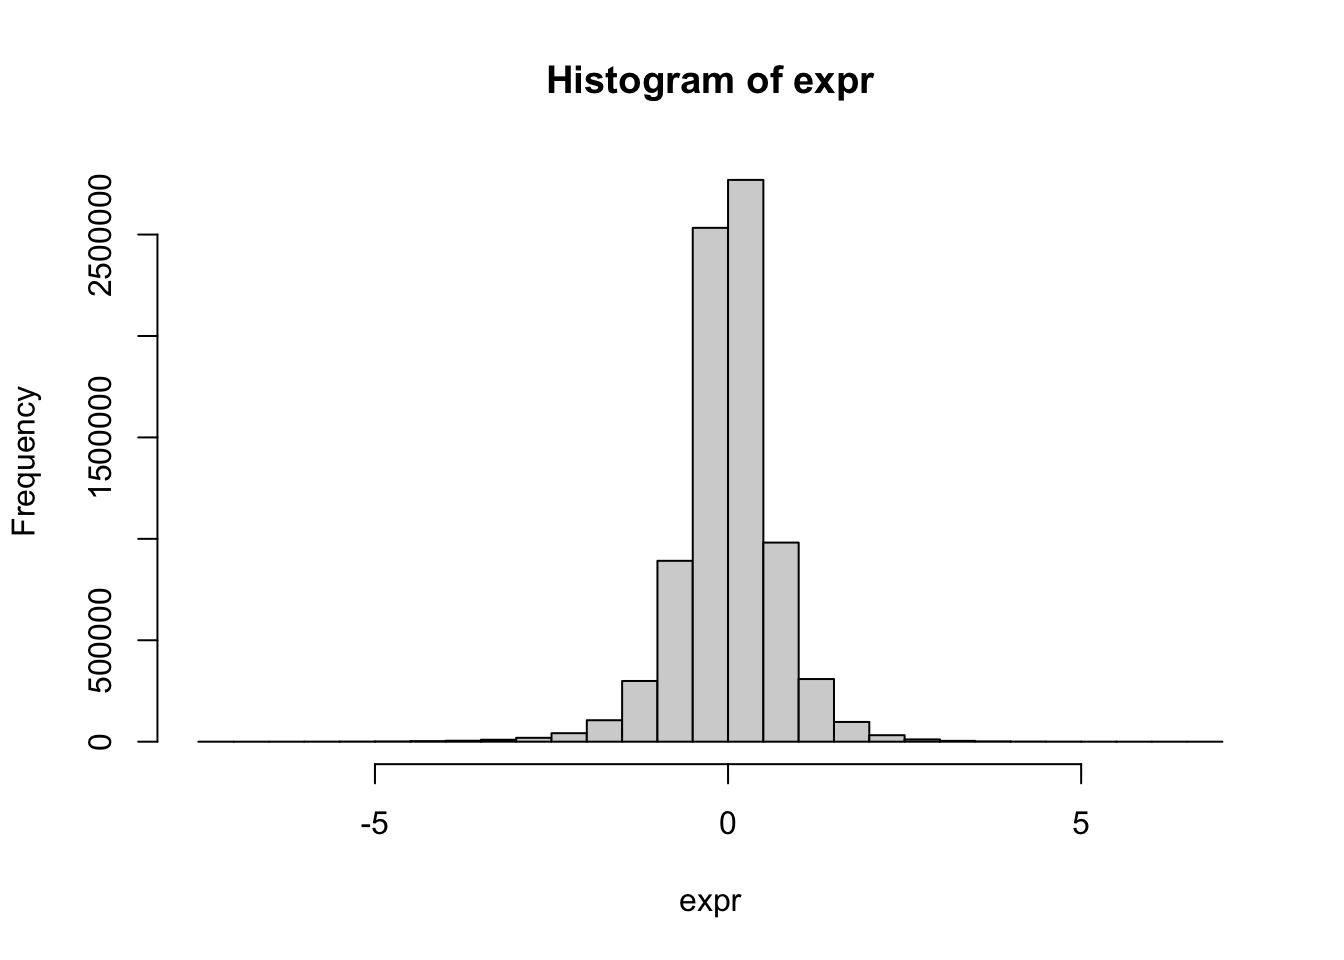
\includegraphics{20210322_REgitim_files/figure-latex/unnamed-chunk-58-1.pdf}

Bu sekilde, hangi bireyin veya genin verisi olduguna bakmaksizin tum degerlerin bir histogramini aliriz. Bu histogram cogu gen ekpresyon verisinde alacaginiz ham veri grafiginden cok farkli, bunun sebebi bunun two channel microarray olmasi ve loess normalizasyonu gibi kimi normalizasyon asamalarindan da gecirilmis olmasi.

Buna bakmak oldukca kolaydi, ama ben genel olarak \texttt{ggplot2} paketinin gorsellestirmelerini kullaniyorum ve herkese en bastan itibaren ggplot ogrenmesini tavsiye ediyorum. Basit grafiklerde biraz zahmetli gelse de kompleks yayina hazir figur olusturmak icin cok ciddi kolaylik sagliyor. \texttt{ggplot2} data.frame objesiyle calisir, oysa bu bir matris. Bu yuzden ufak bir degisiklik yapmamiz lazim:

\begin{Shaded}
\begin{Highlighting}[]
\FunctionTok{library}\NormalTok{(ggplot2)}
\NormalTok{mydat }\OtherTok{=}\NormalTok{ reshape2}\SpecialCharTok{::}\FunctionTok{melt}\NormalTok{(expr)}
\FunctionTok{ggplot}\NormalTok{(mydat, }\FunctionTok{aes}\NormalTok{(}\AttributeTok{x =}\NormalTok{ value)) }\SpecialCharTok{+}
  \FunctionTok{geom\_histogram}\NormalTok{()}
\end{Highlighting}
\end{Shaded}

\begin{verbatim}
## `stat_bin()` using `bins = 30`. Pick better value with `binwidth`.
\end{verbatim}

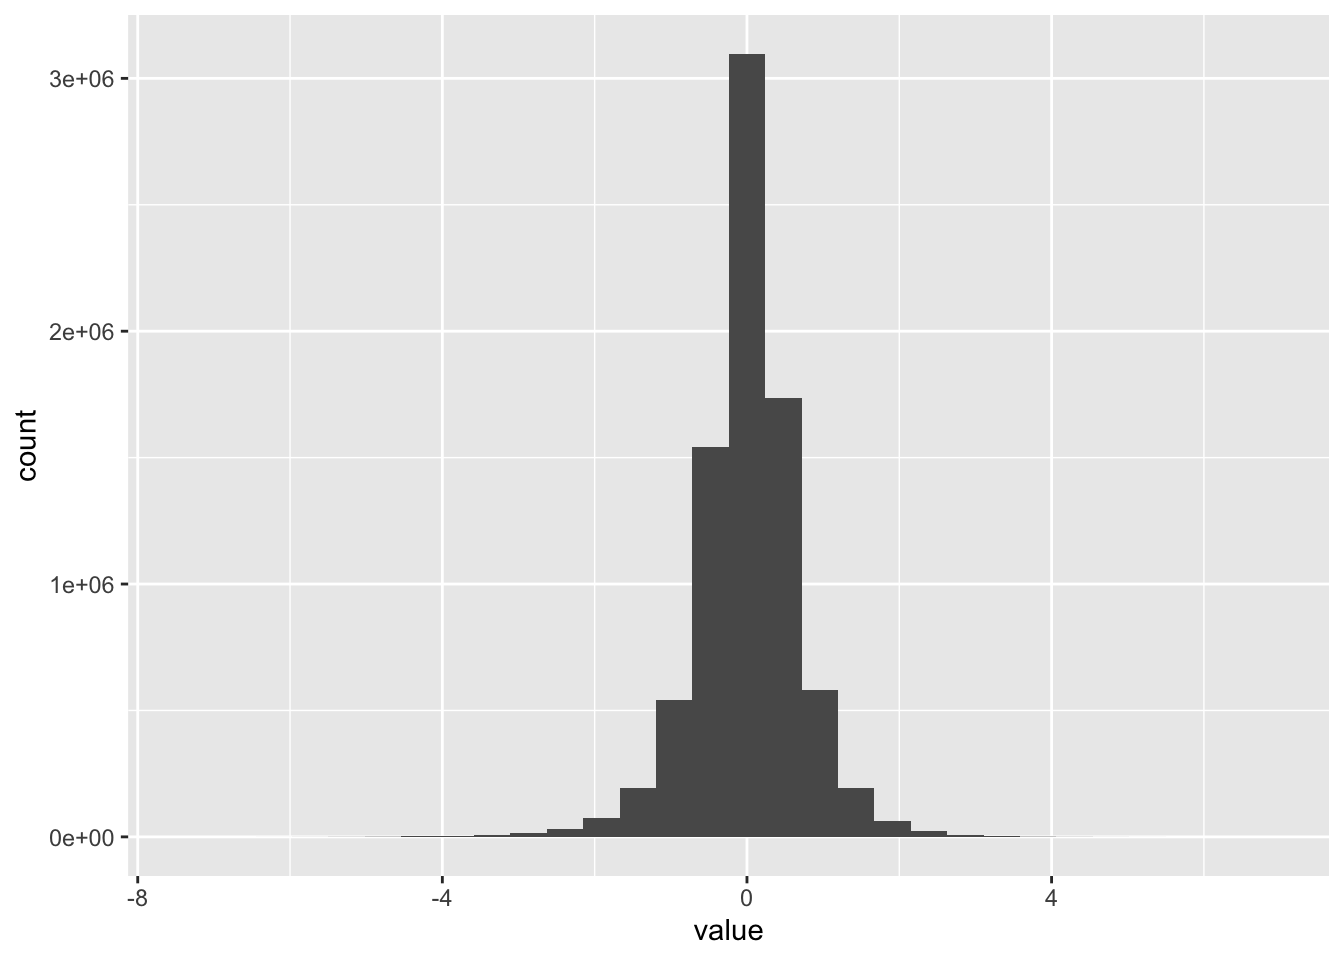
\includegraphics{20210322_REgitim_files/figure-latex/unnamed-chunk-59-1.pdf}

\begin{Shaded}
\begin{Highlighting}[]
\FunctionTok{ggplot}\NormalTok{(mydat, }\FunctionTok{aes}\NormalTok{(}\AttributeTok{x =}\NormalTok{ value)) }\SpecialCharTok{+}
  \FunctionTok{geom\_histogram}\NormalTok{(}\AttributeTok{color =} \StringTok{\textquotesingle{}gray60\textquotesingle{}}\NormalTok{, }\AttributeTok{bins =} \DecValTok{50}\NormalTok{) }\SpecialCharTok{+}
  \FunctionTok{xlab}\NormalTok{(}\StringTok{\textquotesingle{}Probeset Expression\textquotesingle{}}\NormalTok{) }\SpecialCharTok{+}
  \FunctionTok{ylab}\NormalTok{(}\StringTok{\textquotesingle{}Count\textquotesingle{}}\NormalTok{) }\SpecialCharTok{+}
  \FunctionTok{theme\_bw}\NormalTok{()}
\end{Highlighting}
\end{Shaded}

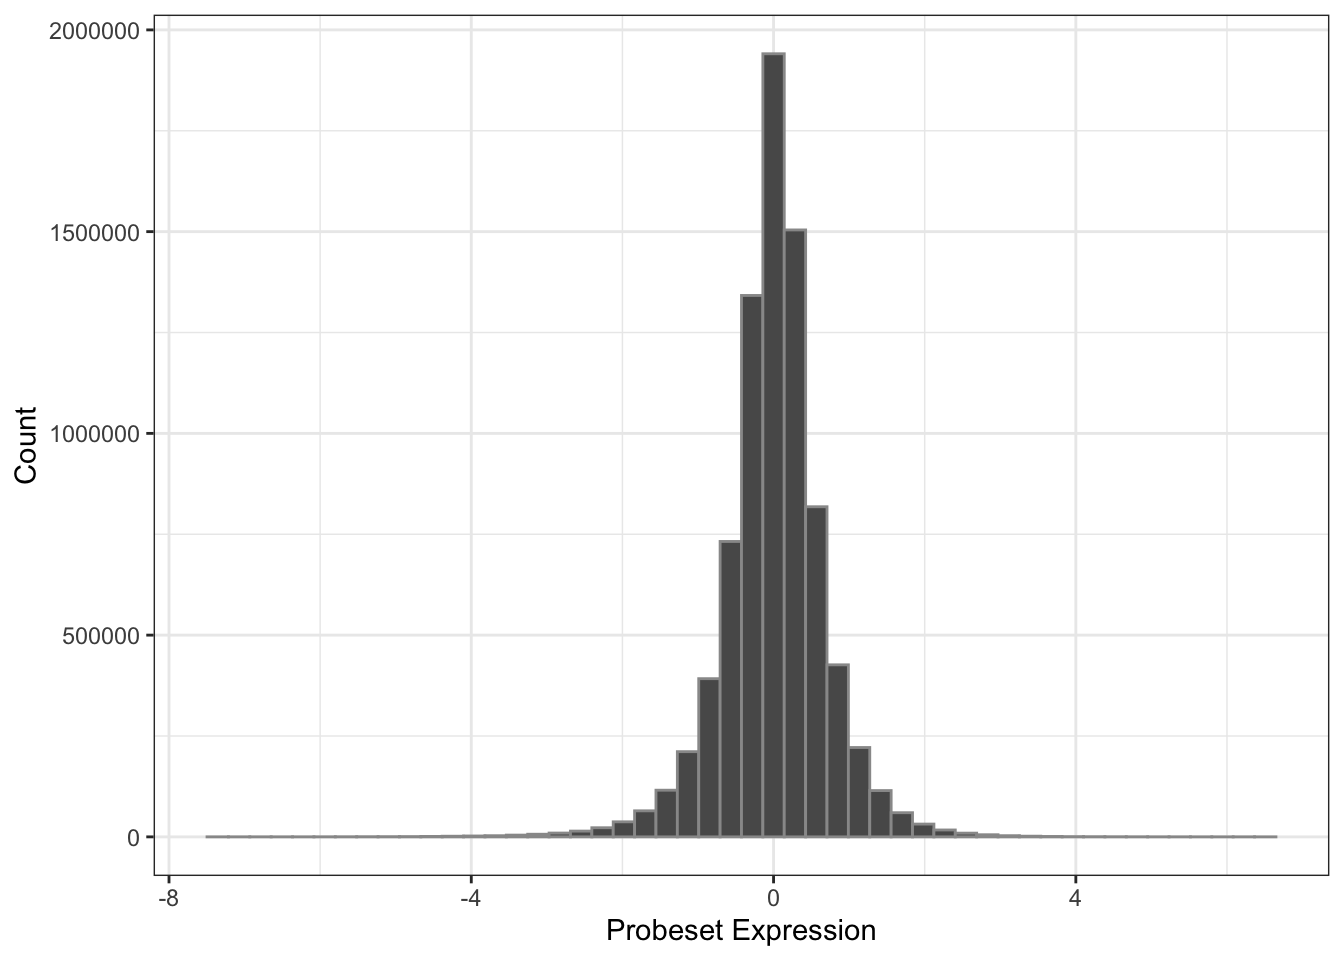
\includegraphics{20210322_REgitim_files/figure-latex/unnamed-chunk-60-1.pdf}

\hypertarget{boxplot}{%
\subsection{Boxplot}\label{boxplot}}

Simdi de ilk birkac bireyin gen anlatim profillerine bakalim. Ilk once base R gorsellestirme fonksiyonu ile:

\begin{Shaded}
\begin{Highlighting}[]
\FunctionTok{boxplot}\NormalTok{(expr[,}\DecValTok{1}\SpecialCharTok{:}\DecValTok{5}\NormalTok{])}
\end{Highlighting}
\end{Shaded}

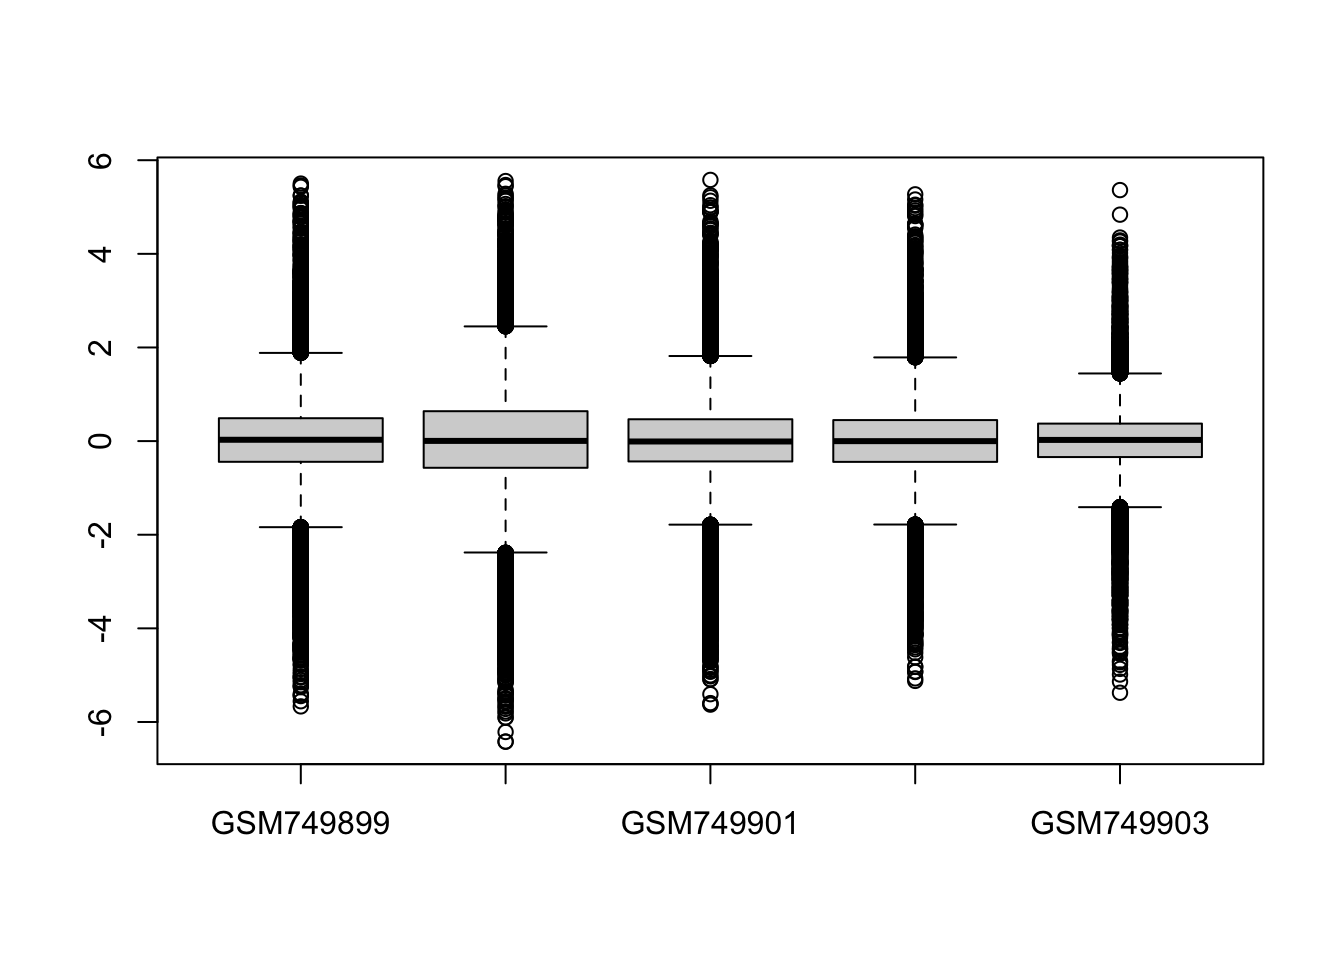
\includegraphics{20210322_REgitim_files/figure-latex/unnamed-chunk-61-1.pdf}

Ayni grafigi ilk bir kac gen icin cizmek isteyecek olsak, hem matrisi subset etmemiz hem de transpoze etmemiz gerekir. Bunu \texttt{t()} fonksiyonu ile kolaylikla yapabiliriz:

\begin{Shaded}
\begin{Highlighting}[]
\FunctionTok{boxplot}\NormalTok{(}\FunctionTok{t}\NormalTok{(expr[}\DecValTok{1}\SpecialCharTok{:}\DecValTok{10}\NormalTok{,]))}
\end{Highlighting}
\end{Shaded}

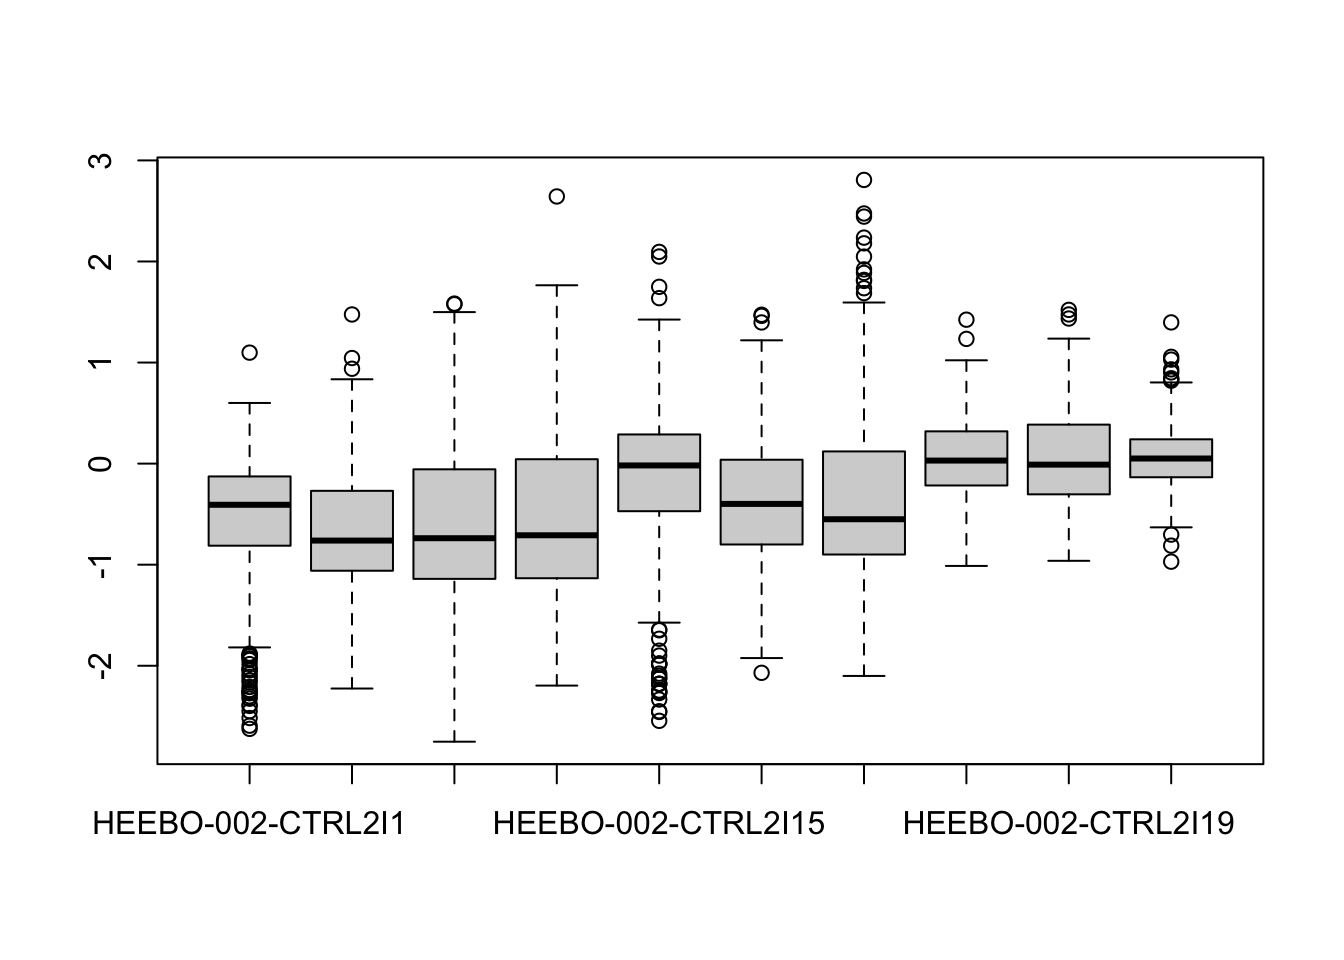
\includegraphics{20210322_REgitim_files/figure-latex/unnamed-chunk-62-1.pdf}

Aynisini ggplot ile yapalim:

\begin{Shaded}
\begin{Highlighting}[]
\NormalTok{mydat }\OtherTok{=}\NormalTok{ reshape2}\SpecialCharTok{::}\FunctionTok{melt}\NormalTok{(expr[,}\DecValTok{1}\SpecialCharTok{:}\DecValTok{5}\NormalTok{])}
\FunctionTok{head}\NormalTok{(mydat)}
\end{Highlighting}
\end{Shaded}

\begin{verbatim}
##                 Var1      Var2     value
## 1  HEEBO-002-CTRL2I1 GSM749899 -1.455124
## 2 HEEBO-002-CTRL2I10 GSM749899  1.044670
## 3 HEEBO-002-CTRL2I11 GSM749899  1.164344
## 4 HEEBO-002-CTRL2I14 GSM749899  1.597227
## 5 HEEBO-002-CTRL2I15 GSM749899 -1.454337
## 6 HEEBO-002-CTRL2I16 GSM749899  1.396667
\end{verbatim}

\begin{Shaded}
\begin{Highlighting}[]
\FunctionTok{ggplot}\NormalTok{(mydat,}\FunctionTok{aes}\NormalTok{(}\AttributeTok{x =}\NormalTok{ Var2, }\AttributeTok{y =}\NormalTok{ value)) }\SpecialCharTok{+}
  \FunctionTok{geom\_boxplot}\NormalTok{(}\AttributeTok{outlier.size =} \FloatTok{0.01}\NormalTok{, }\AttributeTok{outlier.color =} \StringTok{\textquotesingle{}gray\textquotesingle{}}\NormalTok{, }\AttributeTok{color =} \StringTok{\textquotesingle{}darkred\textquotesingle{}}\NormalTok{) }\SpecialCharTok{+}
  \FunctionTok{theme\_bw}\NormalTok{() }\SpecialCharTok{+}
  \FunctionTok{xlab}\NormalTok{(}\ConstantTok{NULL}\NormalTok{) }\SpecialCharTok{+} \FunctionTok{ylab}\NormalTok{(}\StringTok{\textquotesingle{}Probeset Expression Value\textquotesingle{}}\NormalTok{)}
\end{Highlighting}
\end{Shaded}

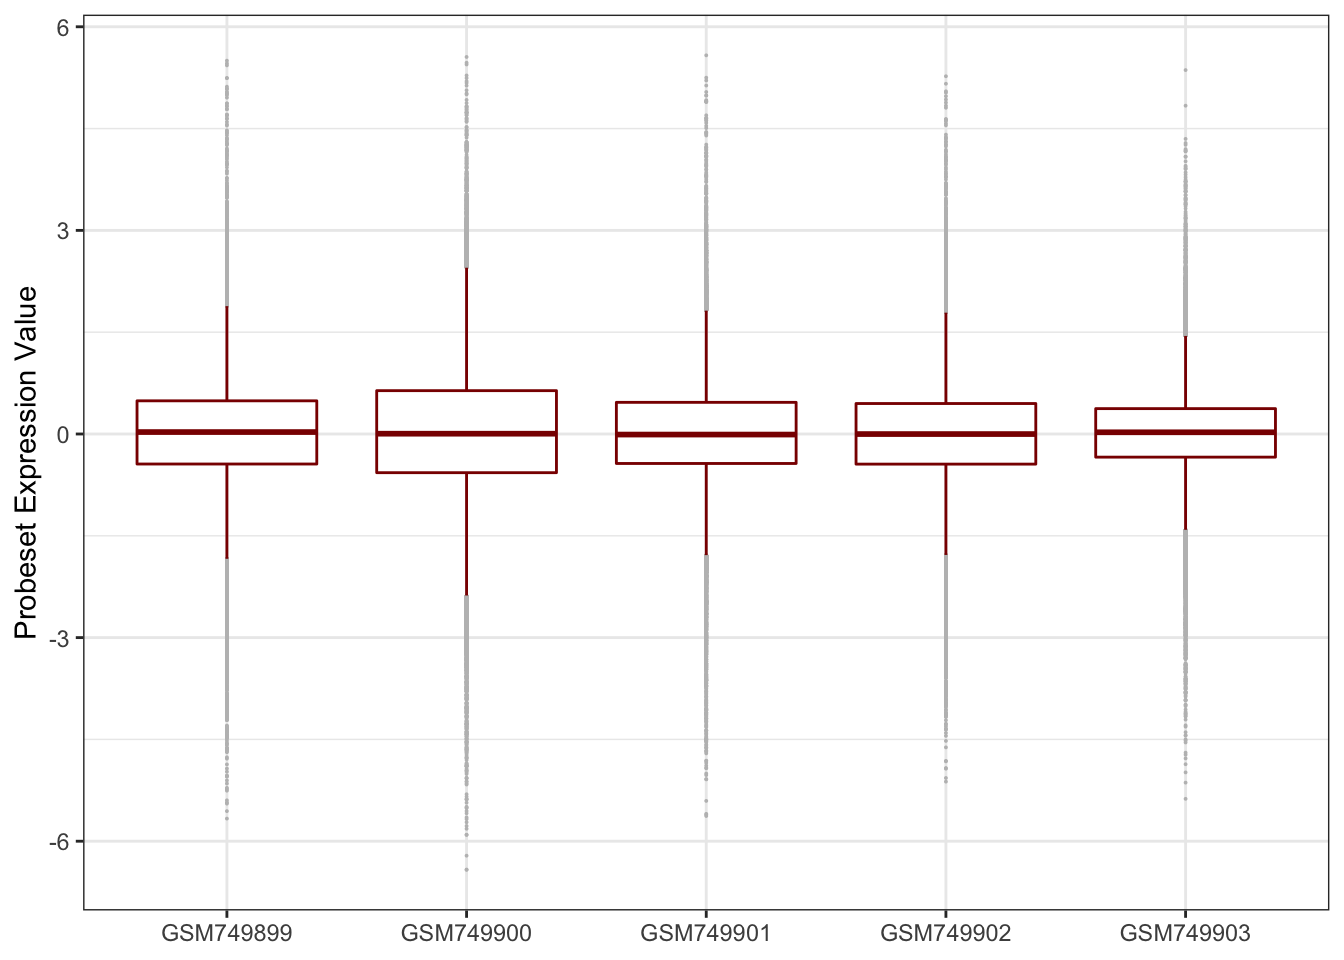
\includegraphics{20210322_REgitim_files/figure-latex/unnamed-chunk-63-1.pdf}

\begin{Shaded}
\begin{Highlighting}[]
\NormalTok{mydat }\OtherTok{=}\NormalTok{ reshape2}\SpecialCharTok{::}\FunctionTok{melt}\NormalTok{(expr[}\DecValTok{1}\SpecialCharTok{:}\DecValTok{5}\NormalTok{,])}
\FunctionTok{head}\NormalTok{(mydat)}
\end{Highlighting}
\end{Shaded}

\begin{verbatim}
##                 Var1      Var2     value
## 1  HEEBO-002-CTRL2I1 GSM749899 -1.455124
## 2 HEEBO-002-CTRL2I10 GSM749899  1.044670
## 3 HEEBO-002-CTRL2I11 GSM749899  1.164344
## 4 HEEBO-002-CTRL2I14 GSM749899  1.597227
## 5 HEEBO-002-CTRL2I15 GSM749899 -1.454337
## 6  HEEBO-002-CTRL2I1 GSM749900 -2.624420
\end{verbatim}

\begin{Shaded}
\begin{Highlighting}[]
\FunctionTok{ggplot}\NormalTok{(mydat,}\FunctionTok{aes}\NormalTok{(}\AttributeTok{x =}\NormalTok{ Var1, }\AttributeTok{y =}\NormalTok{ value)) }\SpecialCharTok{+}
  \FunctionTok{geom\_boxplot}\NormalTok{(}\AttributeTok{outlier.shape=}\ConstantTok{NA}\NormalTok{, }\AttributeTok{color =} \StringTok{\textquotesingle{}darkred\textquotesingle{}}\NormalTok{) }\SpecialCharTok{+}
  \FunctionTok{geom\_jitter}\NormalTok{(}\AttributeTok{size =} \FloatTok{0.5}\NormalTok{, }\AttributeTok{width =} \FloatTok{0.1}\NormalTok{) }\SpecialCharTok{+}
  \FunctionTok{theme\_bw}\NormalTok{() }\SpecialCharTok{+}
  \FunctionTok{xlab}\NormalTok{(}\ConstantTok{NULL}\NormalTok{) }\SpecialCharTok{+} \FunctionTok{ylab}\NormalTok{(}\StringTok{\textquotesingle{}Probeset Expression Value\textquotesingle{}}\NormalTok{)}
\end{Highlighting}
\end{Shaded}

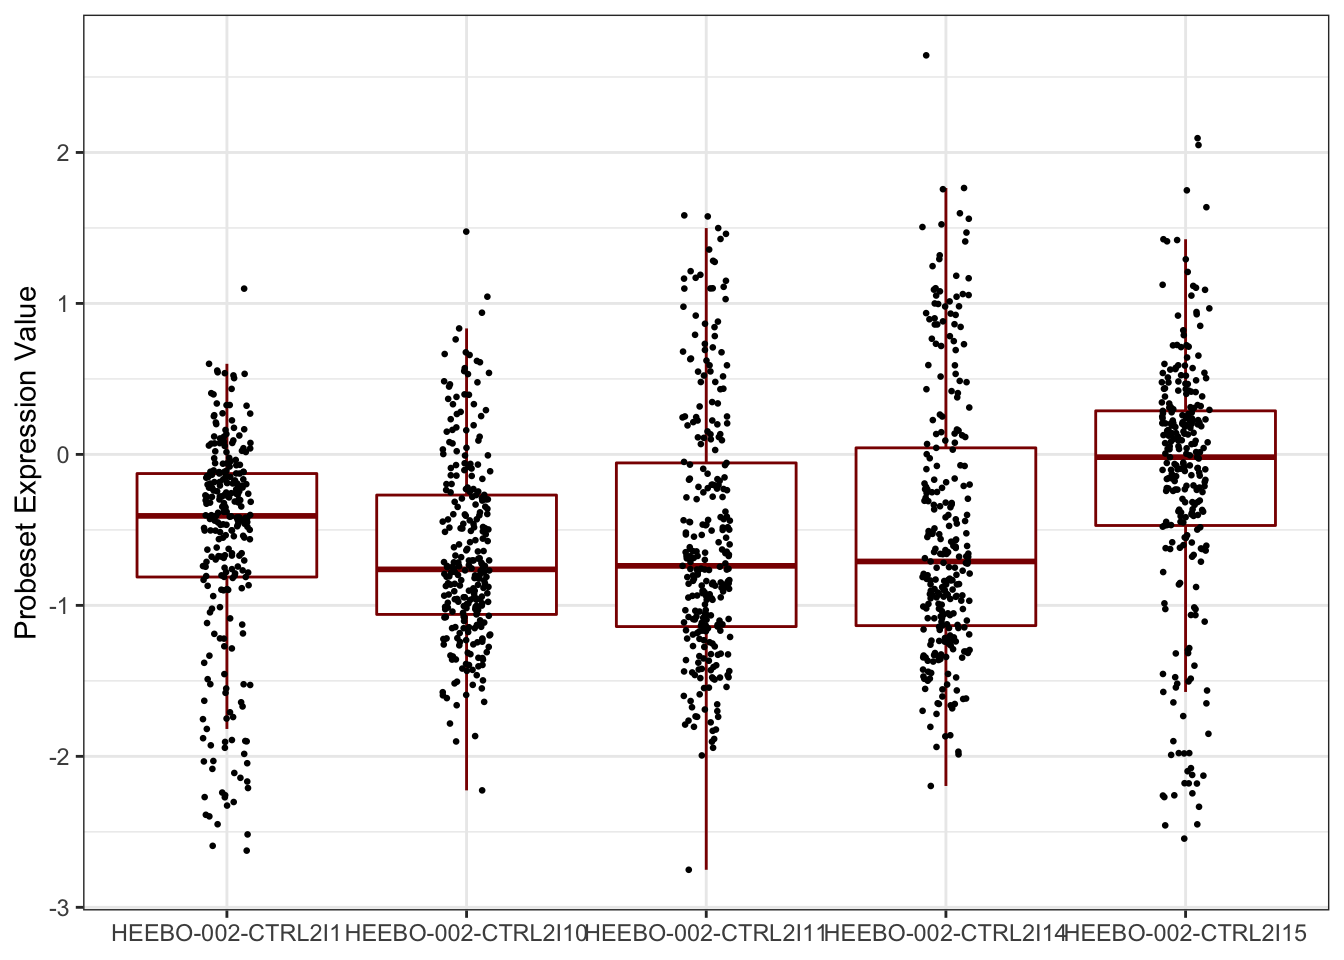
\includegraphics{20210322_REgitim_files/figure-latex/unnamed-chunk-64-1.pdf}

\hypertarget{probesetid---gen-eslestirmesi}{%
\section{ProbesetID - Gen eslestirmesi}\label{probesetid---gen-eslestirmesi}}

Ayni gen ifade verisi gibi probesetID - gen eslesmesi bilgisinin kayitli oldugu bir tablo daha kaydetmistim. Simdi onu okuyalim:

\begin{Shaded}
\begin{Highlighting}[]
\NormalTok{genedata }\OtherTok{=} \FunctionTok{read.csv}\NormalTok{(}\StringTok{\textquotesingle{}https://github.com/mdonertas/20210322\_REgitim/raw/master/data/featuredat.csv\textquotesingle{}}\NormalTok{)}
\NormalTok{genedata[}\DecValTok{1}\SpecialCharTok{:}\DecValTok{3}\NormalTok{,]}
\end{Highlighting}
\end{Shaded}

\begin{verbatim}
##                    X                 ID   OligoID
## 1  HEEBO-002-CTRL2I1  HEEBO-002-CTRL2I1 hCT000577
## 2 HEEBO-002-CTRL2I10 HEEBO-002-CTRL2I10 hCT000586
## 3 HEEBO-002-CTRL2I11 HEEBO-002-CTRL2I11 hCT000587
##                                                                 SEQUENCE
## 1 ACTCTGGATCCTGGGCGACGTCTTCATCGGCCGCTACTACACTGTGTTTGACCGTGACAACAACAGGGTG
## 2 CATCCTCACCGACATCACCAAGGGTGTGCAGTACCTCAACGAGATCAAGGACAGTGTGGTGGCCGGCTTC
## 3 GTCCCTGGAACGCCAGATGCGTGAAATGGAAGAGAACTTTGCCGTTGAAGCTGCTAACTACCAAGACACT
##        GB_ACC Strand Gene_Symbol                                 Gene_Title
## 1 NM_001909.4      +        CTSD                                cathepsin D
## 2 NM_001961.3      +        EEF2 eukaryotic translation elongation factor 2
## 3 NM_003380.3      +         VIM                                   vimentin
##   Entrez_Gene_ID UniGene_Cluster_ID Feb2012_Blast_Cutoffs SPOT_ID
## 1           1509          Hs.654447 100/100_Unique_RefSeq        
## 2           1938          Hs.515070 100/100_Unique_RefSeq        
## 3           7431          Hs.455493 100/100_Unique_RefSeq
\end{verbatim}

\begin{Shaded}
\begin{Highlighting}[]
\FunctionTok{class}\NormalTok{(genedata)}
\end{Highlighting}
\end{Shaded}

\begin{verbatim}
## [1] "data.frame"
\end{verbatim}

Ilk olarak gen bilgisini duzenleyelim. Bunun icin bu data.frame'den iki sutunu kullanacagiz.

\begin{Shaded}
\begin{Highlighting}[]
\NormalTok{genedata}\SpecialCharTok{$}\NormalTok{ID[}\DecValTok{1}\SpecialCharTok{:}\DecValTok{10}\NormalTok{]}
\end{Highlighting}
\end{Shaded}

\begin{verbatim}
##  [1] "HEEBO-002-CTRL2I1"  "HEEBO-002-CTRL2I10" "HEEBO-002-CTRL2I11"
##  [4] "HEEBO-002-CTRL2I14" "HEEBO-002-CTRL2I15" "HEEBO-002-CTRL2I16"
##  [7] "HEEBO-002-CTRL2I17" "HEEBO-002-CTRL2I18" "HEEBO-002-CTRL2I19"
## [10] "HEEBO-002-CTRL2I2"
\end{verbatim}

\begin{Shaded}
\begin{Highlighting}[]
\NormalTok{genedata}\SpecialCharTok{$}\NormalTok{Gene\_Symbol[}\DecValTok{1}\SpecialCharTok{:}\DecValTok{10}\NormalTok{]}
\end{Highlighting}
\end{Shaded}

\begin{verbatim}
##  [1] "CTSD" "EEF2" "VIM"  "VIM"  "GSN"  "EEF2" "VIM"  "CTSD" "RPN2" "RPN2"
\end{verbatim}

Simdi isimlendirilmis bir vektor olusturacagim ki, belli bir probe IDye karsilik gelen geni bulabileyim. Bunu yapmak icin \texttt{setNames()} fonksiyonunu kullanacagim. Isimler, yani ikinci arguman, probeID olacak, vektorun kendisi ise genler, bu sayede vektoru belli bir probe ID kullanarak subset ettigimde hangi gen oldugunu bulabilirim. Buna gecmeden bir ornek:

\begin{Shaded}
\begin{Highlighting}[]
\NormalTok{x }\OtherTok{=} \FunctionTok{setNames}\NormalTok{(}\FunctionTok{c}\NormalTok{(}\DecValTok{1}\SpecialCharTok{:}\DecValTok{3}\NormalTok{),}\FunctionTok{c}\NormalTok{(}\StringTok{\textquotesingle{}bir\textquotesingle{}}\NormalTok{,}\StringTok{\textquotesingle{}iki\textquotesingle{}}\NormalTok{,}\StringTok{\textquotesingle{}uc\textquotesingle{}}\NormalTok{))}
\NormalTok{x}
\end{Highlighting}
\end{Shaded}

\begin{verbatim}
## bir iki  uc 
##   1   2   3
\end{verbatim}

ikinci elemani almak icin:

\begin{Shaded}
\begin{Highlighting}[]
\NormalTok{x[}\DecValTok{2}\NormalTok{]}
\end{Highlighting}
\end{Shaded}

\begin{verbatim}
## iki 
##   2
\end{verbatim}

\begin{Shaded}
\begin{Highlighting}[]
\NormalTok{x[}\StringTok{\textquotesingle{}iki\textquotesingle{}}\NormalTok{]}
\end{Highlighting}
\end{Shaded}

\begin{verbatim}
## iki 
##   2
\end{verbatim}

Bunlarin ikisini de kullanabiliyorum. IDleri kullanarak genleri bulmam da ayni sekilde olacak:

\begin{Shaded}
\begin{Highlighting}[]
\NormalTok{genemap }\OtherTok{=} \FunctionTok{setNames}\NormalTok{(genedata}\SpecialCharTok{$}\NormalTok{Gene\_Symbol,genedata}\SpecialCharTok{$}\NormalTok{ID)}
\NormalTok{genemap[}\DecValTok{1}\SpecialCharTok{:}\DecValTok{5}\NormalTok{]}
\end{Highlighting}
\end{Shaded}

\begin{verbatim}
##  HEEBO-002-CTRL2I1 HEEBO-002-CTRL2I10 HEEBO-002-CTRL2I11 HEEBO-002-CTRL2I14 
##             "CTSD"             "EEF2"              "VIM"              "VIM" 
## HEEBO-002-CTRL2I15 
##              "GSN"
\end{verbatim}

\begin{Shaded}
\begin{Highlighting}[]
\FunctionTok{head}\NormalTok{(genemap)}
\end{Highlighting}
\end{Shaded}

\begin{verbatim}
##  HEEBO-002-CTRL2I1 HEEBO-002-CTRL2I10 HEEBO-002-CTRL2I11 HEEBO-002-CTRL2I14 
##             "CTSD"             "EEF2"              "VIM"              "VIM" 
## HEEBO-002-CTRL2I15 HEEBO-002-CTRL2I16 
##              "GSN"             "EEF2"
\end{verbatim}

Matrisin satir isimleriyle genemap'i subset ettigimiz zaman, dogru sirayla hangi genlere karsilik geliyorsa bize bu bilgiyi verecek. Simdi once bir yanlis yapma ihtimalimize karsin matrisimizi kopyalayalim:

\begin{Shaded}
\begin{Highlighting}[]
\NormalTok{expr\_yedek }\OtherTok{=}\NormalTok{ expr}
\end{Highlighting}
\end{Shaded}

Simdi ilk olarak bir probeset ID birden fazla genle eslesiyor mu buna bakmaliyiz, bunlar veri duplikasyonu yaratacagindan istatistiksel test yapmamizi zorlastirir bunlari veriden cikararak baslayacagiz:

\begin{Shaded}
\begin{Highlighting}[]
\FunctionTok{any}\NormalTok{(}\FunctionTok{duplicated}\NormalTok{(}\FunctionTok{names}\NormalTok{(genemap)))}
\end{Highlighting}
\end{Shaded}

\begin{verbatim}
## [1] FALSE
\end{verbatim}

Hic tekrar eden bir probesetIDmiz yok - yani bu bu veriseti icin problem degil. Bir de cok fazla sayida probesetIDye map olmus olan genlere bakalim:

\begin{Shaded}
\begin{Highlighting}[]
\FunctionTok{sort}\NormalTok{(}\FunctionTok{table}\NormalTok{(genemap),}\AttributeTok{dec=}\NormalTok{T)[}\DecValTok{1}\SpecialCharTok{:}\DecValTok{10}\NormalTok{]}
\end{Highlighting}
\end{Shaded}

\begin{verbatim}
## genemap
## ##noname##                  LRP1       OCRL       TLN1        TTN      CDH23 
##        903        825         88         62         55         55         41 
##      ANXA7        RB1      DNAH9 
##         40         40         37
\end{verbatim}

Bunlardan \texttt{\textquotesingle{}\#\#noname\#\#} ve \texttt{\textquotesingle{}\textquotesingle{}} tabii ki gen ismi degil. Bunlari veriden cikartmak gerekir, ama bunu matrixe isimleri gecirdikten sonra yapacagim. Simdi probeset IDleri gen isimleriyle degistirerek devam edelim:

\begin{Shaded}
\begin{Highlighting}[]
\FunctionTok{rownames}\NormalTok{(expr) }\OtherTok{=}\NormalTok{ genemap[}\FunctionTok{rownames}\NormalTok{(expr)]}
\end{Highlighting}
\end{Shaded}

\begin{Shaded}
\begin{Highlighting}[]
\NormalTok{expr[}\DecValTok{1}\SpecialCharTok{:}\DecValTok{5}\NormalTok{,}\DecValTok{1}\SpecialCharTok{:}\DecValTok{5}\NormalTok{]}
\end{Highlighting}
\end{Shaded}

\begin{verbatim}
##      GSM749899  GSM749900 GSM749901  GSM749902  GSM749903
## CTSD -1.455124 -2.6244200 -1.904436 -1.5793507 -2.1666262
## EEF2  1.044670  0.4490985  0.619243  0.1930628 -0.4370544
## VIM   1.164344  1.5833201  1.150024  1.5764080  1.3569308
## VIM   1.597227  1.4105770  1.469449  2.6433802  1.7567335
## GSN  -1.454337 -1.9784923 -1.485409 -1.5038039 -1.2828650
\end{verbatim}

\begin{Shaded}
\begin{Highlighting}[]
\FunctionTok{sort}\NormalTok{(}\FunctionTok{table}\NormalTok{(}\FunctionTok{rownames}\NormalTok{(expr)), }\AttributeTok{dec =}\NormalTok{ T)[}\DecValTok{1}\SpecialCharTok{:}\DecValTok{10}\NormalTok{]}
\end{Highlighting}
\end{Shaded}

\begin{verbatim}
## 
## ##noname##                  LRP1       OCRL       TLN1        TTN      CDH23 
##        903        825         88         62         55         55         41 
##      ANXA7        RB1      DNAH9 
##         40         40         37
\end{verbatim}

Burada gordugunuz gibi bazi gen isimleri birden fazla kez tekrar ediliyor. Bu mikrodizin dizaynindan kaynakli bir durum, her gen bir ya da daha fazla probeset ile temsil ediliyor. Genelde her gen bu probesetlerin ortalamasi ya da maksimumu alinarak ozetlenir - bu sayede her gen matriste bir defa yer alir. Bunu yapmak icin matrisi gen isimleriyle subset etmeyi ogrenecegiz. Zaten belli bir isimle subset yapmayi biliyoruz, ancak bu sadece tekrarli olmayan durumlarda gecerli. Suna bakalim:

\begin{Shaded}
\begin{Highlighting}[]
\NormalTok{x }\OtherTok{=} \FunctionTok{setNames}\NormalTok{(}\FunctionTok{c}\NormalTok{(}\DecValTok{1}\SpecialCharTok{:}\DecValTok{5}\NormalTok{), }\FunctionTok{c}\NormalTok{(}\StringTok{\textquotesingle{}bir\textquotesingle{}}\NormalTok{,}\StringTok{\textquotesingle{}iki\textquotesingle{}}\NormalTok{,}\StringTok{\textquotesingle{}iki\textquotesingle{}}\NormalTok{,}\StringTok{\textquotesingle{}dort\textquotesingle{}}\NormalTok{,}\StringTok{\textquotesingle{}bes\textquotesingle{}}\NormalTok{))}
\NormalTok{x[}\StringTok{\textquotesingle{}iki\textquotesingle{}}\NormalTok{]}
\end{Highlighting}
\end{Shaded}

\begin{verbatim}
## iki 
##   2
\end{verbatim}

oysa 3 degerine sahip olan elemanin adi da `iki'. Bu tarz tekrarli durumlarda otomatik olarak ilk eleman verilir. Ikisini birden istiyorsak subset islemini \texttt{\%in\%} operatoru ile yapmamiz gerekir.

\hypertarget{in-operatoru}{%
\subsection{\texorpdfstring{\texttt{\%in\%} operatoru}{\%in\% operatoru}}\label{in-operatoru}}

\begin{Shaded}
\begin{Highlighting}[]
\StringTok{\textquotesingle{}elma\textquotesingle{}} \SpecialCharTok{\%in\%} \FunctionTok{c}\NormalTok{(}\StringTok{\textquotesingle{}elma\textquotesingle{}}\NormalTok{,}\StringTok{\textquotesingle{}armut\textquotesingle{}}\NormalTok{)}
\end{Highlighting}
\end{Shaded}

\begin{verbatim}
## [1] TRUE
\end{verbatim}

\begin{Shaded}
\begin{Highlighting}[]
\StringTok{\textquotesingle{}muz\textquotesingle{}} \SpecialCharTok{\%in\%} \FunctionTok{c}\NormalTok{(}\StringTok{\textquotesingle{}elma\textquotesingle{}}\NormalTok{,}\StringTok{\textquotesingle{}armut\textquotesingle{}}\NormalTok{)}
\end{Highlighting}
\end{Shaded}

\begin{verbatim}
## [1] FALSE
\end{verbatim}

\begin{Shaded}
\begin{Highlighting}[]
\FunctionTok{c}\NormalTok{(}\StringTok{\textquotesingle{}elma\textquotesingle{}}\NormalTok{, }\StringTok{\textquotesingle{}muz\textquotesingle{}}\NormalTok{) }\SpecialCharTok{\%in\%} \StringTok{\textquotesingle{}elma\textquotesingle{}}
\end{Highlighting}
\end{Shaded}

\begin{verbatim}
## [1]  TRUE FALSE
\end{verbatim}

\begin{Shaded}
\begin{Highlighting}[]
\FunctionTok{c}\NormalTok{(}\StringTok{\textquotesingle{}elma\textquotesingle{}}\NormalTok{, }\StringTok{\textquotesingle{}muz\textquotesingle{}}\NormalTok{) }\SpecialCharTok{\%in\%} \StringTok{\textquotesingle{}muz\textquotesingle{}}
\end{Highlighting}
\end{Shaded}

\begin{verbatim}
## [1] FALSE  TRUE
\end{verbatim}

Bilmemiz gereken bir konu da bir vektoru ya da matrisi mantiksal degiskenlerle de subset edebildigimiz:

\begin{Shaded}
\begin{Highlighting}[]
\FunctionTok{c}\NormalTok{(}\DecValTok{1}\SpecialCharTok{:}\DecValTok{5}\NormalTok{)[}\FunctionTok{c}\NormalTok{(T,T,F,T,F)]}
\end{Highlighting}
\end{Shaded}

\begin{verbatim}
## [1] 1 2 4
\end{verbatim}

Ilk olarak gen ismi olarak \texttt{\textquotesingle{}\#\#noname\#\#} ve \texttt{\textquotesingle{}\textquotesingle{}} gorunen satirlari veriden cikartarak baslamaliyiz:

\begin{Shaded}
\begin{Highlighting}[]
\NormalTok{expr }\OtherTok{=}\NormalTok{ expr[}\SpecialCharTok{!}\FunctionTok{rownames}\NormalTok{(expr) }\SpecialCharTok{\%in\%} \FunctionTok{c}\NormalTok{(}\StringTok{\textquotesingle{}\#\#noname\#\#\textquotesingle{}}\NormalTok{,}\StringTok{\textquotesingle{}\textquotesingle{}}\NormalTok{),]}
\end{Highlighting}
\end{Shaded}

\begin{Shaded}
\begin{Highlighting}[]
\FunctionTok{sort}\NormalTok{(}\FunctionTok{table}\NormalTok{(}\FunctionTok{rownames}\NormalTok{(expr)),}\AttributeTok{dec=}\NormalTok{T)[}\DecValTok{1}\SpecialCharTok{:}\DecValTok{10}\NormalTok{]}
\end{Highlighting}
\end{Shaded}

\begin{verbatim}
## 
##  LRP1  OCRL  TLN1   TTN CDH23 ANXA7   RB1 DNAH9 WDFY3 SYNE2 
##    88    62    55    55    41    40    40    37    37    36
\end{verbatim}

Simdi tekrar eden genleri ozetlemeye geri donelim.

\begin{Shaded}
\begin{Highlighting}[]
\NormalTok{expr[}\FunctionTok{rownames}\NormalTok{(expr) }\SpecialCharTok{\%in\%} \StringTok{\textquotesingle{}VIM\textquotesingle{}}\NormalTok{, }\DecValTok{1}\SpecialCharTok{:}\DecValTok{5}\NormalTok{]}
\end{Highlighting}
\end{Shaded}

\begin{verbatim}
##     GSM749899 GSM749900 GSM749901 GSM749902 GSM749903
## VIM  1.164344  1.583320  1.150024  1.576408  1.356931
## VIM  1.597227  1.410577  1.469449  2.643380  1.756734
## VIM  2.475041  2.236114  2.179526  2.807048  2.443889
## VIM  2.414010  2.242931  2.379348  1.909755  2.596801
## VIM  2.913906  1.343048  2.536056  2.271887  2.118884
## VIM  1.743049  1.492585  1.621053  1.394594  2.030154
## VIM  1.171174  1.165681  1.099818  2.274270  1.541334
## VIM  1.446696  1.451936  1.782307  2.605349  1.957581
## VIM  1.131674  1.172329  1.053107  1.871871  1.780982
\end{verbatim}

Simdi yeni bir fonksiyon ogrenelim \texttt{colMeans()} bu da adi ustunde sutun ortalamasini aliyor. Yani matrisi tum VIM genine karsilik gelen probesetler icin subset edip, \texttt{colMeans()} dersek tek boyutlu, satirlarin ortalamasina sahip bir vektor verecek:

\begin{Shaded}
\begin{Highlighting}[]
\NormalTok{vimmeans }\OtherTok{=} \FunctionTok{colMeans}\NormalTok{(expr[}\FunctionTok{rownames}\NormalTok{(expr) }\SpecialCharTok{\%in\%} \StringTok{\textquotesingle{}VIM\textquotesingle{}}\NormalTok{, ])}
\FunctionTok{head}\NormalTok{(vimmeans)}
\end{Highlighting}
\end{Shaded}

\begin{verbatim}
## GSM749899 GSM749900 GSM749901 GSM749902 GSM749903 GSM749904 
##  1.784125  1.566502  1.696743  2.150507  1.953699  1.409357
\end{verbatim}

Ama bu sadece tek bir gen icin. Oysa biz tek genle ilgilenmiyoruz, butun genler icin bunu yapmak istiyoruz. Eger programlama dillerine asinaysaniz \texttt{for} loop larini duymussunuzdur. Bunlar ayni islemin defalarca ayni ya da farkli inputlar icin tekrarlanmasini saglar. R'da da for loop yazabiliriz bunun icin kullanilacak fonksiyon \texttt{for}. Bizse for yerine R'a ozgu *apply fonksiyonlari olarak gecen fonksiyonlardan biri olan \texttt{sapply()} fonksiyonu ile bunu yapacagiz. Ilk olarak butun gen isimlerini almaliyiz. Bunu sadece \texttt{rownames()} ile alamiyoruz cunku isimler tekrar ediyor. Onun yerine her degerin sadece bir kere tekrar edilmesini \texttt{unique()} fonksiyonu ile saglayacagiz.

\begin{Shaded}
\begin{Highlighting}[]
\NormalTok{genisimleri }\OtherTok{=} \FunctionTok{unique}\NormalTok{(}\FunctionTok{rownames}\NormalTok{(expr))}
\FunctionTok{nrow}\NormalTok{(expr)}
\end{Highlighting}
\end{Shaded}

\begin{verbatim}
## [1] 28448
\end{verbatim}

\begin{Shaded}
\begin{Highlighting}[]
\FunctionTok{length}\NormalTok{(genisimleri)}
\end{Highlighting}
\end{Shaded}

\begin{verbatim}
## [1] 17160
\end{verbatim}

Sadece 17bin gen var. Yani her gen cok defa tekrar ediliyor olmak zorunda degil. Eger tekrar edilmeyen bir geni subset edersek, `sutun ortalamalarini ver' demek icin kullanacagimiz \texttt{colMeans} fonksiyonu calismaz, cunku bir matris degil bir vektor soz konusu olacak. Bunun icin bir de \texttt{if} fonksiyonunu ogrenmeliyiz. \texttt{if} bir kodu ancak belli kosullar altinda calistiracaktir. Bu sayede eger bir defa geciyorsa sunu yap, birden fazla kez tekrar ediliyorsa sunu yap seklinde bir kod yazmamiz mumkun olacak. If'e cok kisa bir ornek:

\begin{Shaded}
\begin{Highlighting}[]
\NormalTok{vektorum }\OtherTok{=} \FunctionTok{c}\NormalTok{(}\StringTok{\textquotesingle{}elma\textquotesingle{}}\NormalTok{,}\StringTok{\textquotesingle{}muz\textquotesingle{}}\NormalTok{,}\StringTok{\textquotesingle{}armut\textquotesingle{}}\NormalTok{)}
\ControlFlowTok{if}\NormalTok{(}\StringTok{\textquotesingle{}cilek\textquotesingle{}}\SpecialCharTok{\%in\%}\NormalTok{vektorum)\{}
  \FunctionTok{print}\NormalTok{(}\StringTok{\textquotesingle{}cilek var!\textquotesingle{}}\NormalTok{)}
\NormalTok{\} }\ControlFlowTok{else} \ControlFlowTok{if}\NormalTok{(}\StringTok{\textquotesingle{}elma\textquotesingle{}} \SpecialCharTok{\%in\%}\NormalTok{ vektorum)\{}
  \FunctionTok{print}\NormalTok{(}\StringTok{\textquotesingle{}elma var!\textquotesingle{}}\NormalTok{)}
\NormalTok{\} }\ControlFlowTok{else}\NormalTok{\{}
  \FunctionTok{print}\NormalTok{(}\StringTok{\textquotesingle{}ne cilek ne elma var :(\textquotesingle{}}\NormalTok{)}
\NormalTok{\}}
\end{Highlighting}
\end{Shaded}

\begin{verbatim}
## [1] "elma var!"
\end{verbatim}

daha iyi anlayabilmemiz icin bir ornek daha:

\begin{Shaded}
\begin{Highlighting}[]
\NormalTok{vektorum }\OtherTok{=} \FunctionTok{c}\NormalTok{(}\StringTok{\textquotesingle{}elma\textquotesingle{}}\NormalTok{,}\StringTok{\textquotesingle{}muz\textquotesingle{}}\NormalTok{,}\StringTok{\textquotesingle{}armut\textquotesingle{}}\NormalTok{)}
\ControlFlowTok{if}\NormalTok{(}\StringTok{\textquotesingle{}muz\textquotesingle{}}\SpecialCharTok{\%in\%}\NormalTok{vektorum)\{}
  \FunctionTok{print}\NormalTok{(}\StringTok{\textquotesingle{}muz var!\textquotesingle{}}\NormalTok{)}
\NormalTok{\} }\ControlFlowTok{else} \ControlFlowTok{if}\NormalTok{(}\StringTok{\textquotesingle{}elma\textquotesingle{}} \SpecialCharTok{\%in\%}\NormalTok{ vektorum)\{}
  \FunctionTok{print}\NormalTok{(}\StringTok{\textquotesingle{}elma var!\textquotesingle{}}\NormalTok{)}
\NormalTok{\} }\ControlFlowTok{else}\NormalTok{\{}
  \FunctionTok{print}\NormalTok{(}\StringTok{\textquotesingle{}ne cilek ne elma var :(\textquotesingle{}}\NormalTok{)}
\NormalTok{\}}
\end{Highlighting}
\end{Shaded}

\begin{verbatim}
## [1] "muz var!"
\end{verbatim}

hem elma hem muz olmasina ragmen sadece birinci komut calisti. Bunun sebebi \texttt{else} komutu ancak ilk kodumuz yanlissa calisacak olmasi.

Simdi de cok kisa \texttt{sapply()} nasil calisiyor buna bakalim:

\begin{Shaded}
\begin{Highlighting}[]
\FunctionTok{sapply}\NormalTok{(}\FunctionTok{c}\NormalTok{(}\DecValTok{1}\SpecialCharTok{:}\DecValTok{10}\NormalTok{),}\ControlFlowTok{function}\NormalTok{(i)\{}
\NormalTok{  i }\SpecialCharTok{*} \DecValTok{2}
\NormalTok{\})}
\end{Highlighting}
\end{Shaded}

\begin{verbatim}
##  [1]  2  4  6  8 10 12 14 16 18 20
\end{verbatim}

\begin{Shaded}
\begin{Highlighting}[]
\FunctionTok{sapply}\NormalTok{(}\FunctionTok{c}\NormalTok{(}\DecValTok{1}\SpecialCharTok{:}\DecValTok{10}\NormalTok{),}\ControlFlowTok{function}\NormalTok{(i)\{}
\NormalTok{  i }\SpecialCharTok{*}\NormalTok{ (i}\DecValTok{{-}1}\NormalTok{)}
\NormalTok{\})}
\end{Highlighting}
\end{Shaded}

\begin{verbatim}
##  [1]  0  2  6 12 20 30 42 56 72 90
\end{verbatim}

Simdi biraz ileri duzey gibi gorunmesi muhtemel bir kod yazacagiz ama basamak basamak inceleyince anlasilmasi kolay olacaktir:

\begin{Shaded}
\begin{Highlighting}[]
\NormalTok{genexpr }\OtherTok{=} \FunctionTok{sapply}\NormalTok{(genisimleri, }\ControlFlowTok{function}\NormalTok{(gen) \{}
\NormalTok{  i }\OtherTok{=} \FunctionTok{rownames}\NormalTok{(expr)}\SpecialCharTok{\%in\%}\NormalTok{gen}
  \ControlFlowTok{if}\NormalTok{(}\FunctionTok{sum}\NormalTok{(i)}\SpecialCharTok{\textgreater{}}\DecValTok{1}\NormalTok{)\{}
    \FunctionTok{colMeans}\NormalTok{(expr[i,])}
\NormalTok{  \} }\ControlFlowTok{else} \ControlFlowTok{if}\NormalTok{(}\FunctionTok{sum}\NormalTok{(i)}\SpecialCharTok{==}\DecValTok{1}\NormalTok{)\{}
\NormalTok{    expr[i,]}
\NormalTok{  \}}
\NormalTok{\})}
\end{Highlighting}
\end{Shaded}

\begin{Shaded}
\begin{Highlighting}[]
\NormalTok{genexpr[}\DecValTok{1}\SpecialCharTok{:}\DecValTok{5}\NormalTok{,}\DecValTok{1}\SpecialCharTok{:}\DecValTok{5}\NormalTok{]}
\end{Highlighting}
\end{Shaded}

\begin{verbatim}
##                 CTSD      EEF2      VIM        GSN     RPN2
## GSM749899 -0.8124619 1.5620237 1.784125 -0.6578933 1.658038
## GSM749900 -1.3310489 1.4339156 1.566502 -1.1007844 1.528385
## GSM749901 -1.2447029 0.9832866 1.696743 -1.0306526 1.286318
## GSM749902 -1.2017866 0.7393814 2.150507 -0.8413292 1.153392
## GSM749903 -1.1041998 0.2957918 1.953699 -0.7242716 0.789019
\end{verbatim}

satir-sutun yer degistirmis durumda. bunu yine transpoze ederek duzeltebiliriz:

\begin{Shaded}
\begin{Highlighting}[]
\NormalTok{genexpr }\OtherTok{=} \FunctionTok{t}\NormalTok{(genexpr)}
\end{Highlighting}
\end{Shaded}

\begin{Shaded}
\begin{Highlighting}[]
\NormalTok{genexpr[}\DecValTok{1}\SpecialCharTok{:}\DecValTok{5}\NormalTok{,}\DecValTok{1}\SpecialCharTok{:}\DecValTok{5}\NormalTok{]}
\end{Highlighting}
\end{Shaded}

\begin{verbatim}
##       GSM749899 GSM749900  GSM749901  GSM749902  GSM749903
## CTSD -0.8124619 -1.331049 -1.2447029 -1.2017866 -1.1041998
## EEF2  1.5620237  1.433916  0.9832866  0.7393814  0.2957918
## VIM   1.7841245  1.566502  1.6967431  2.1505070  1.9536987
## GSN  -0.6578933 -1.100784 -1.0306526 -0.8413292 -0.7242716
## RPN2  1.6580375  1.528385  1.2863177  1.1533917  0.7890190
\end{verbatim}

\begin{Shaded}
\begin{Highlighting}[]
\FunctionTok{dim}\NormalTok{(genexpr)}
\end{Highlighting}
\end{Shaded}

\begin{verbatim}
## [1] 17160   269
\end{verbatim}

Artik her gen icin bir satirimiz var!

\hypertarget{quantile-normalization}{%
\section{Quantile Normalization}\label{quantile-normalization}}

Son olarak bu gen ifade matrixinde bir normalizasyon metodu uygulayalim. Burada amacimiz farkli ornekler arasindaki olasi teknik varyasyonu ortadan kaldirmak. Uygulayacagimiz normalizasyonun adi `quantile normalization' - bunun sonunda tum orneklerin dagilimlari ayni olacak - genler farkli degerler alacak ama genlerin dagilimi ayni olacak. Normalizasyon oncesi ilk bir kac bireyin dagilimina bakalim.

\begin{Shaded}
\begin{Highlighting}[]
\FunctionTok{boxplot}\NormalTok{(genexpr[,}\DecValTok{1}\SpecialCharTok{:}\DecValTok{20}\NormalTok{])}
\end{Highlighting}
\end{Shaded}

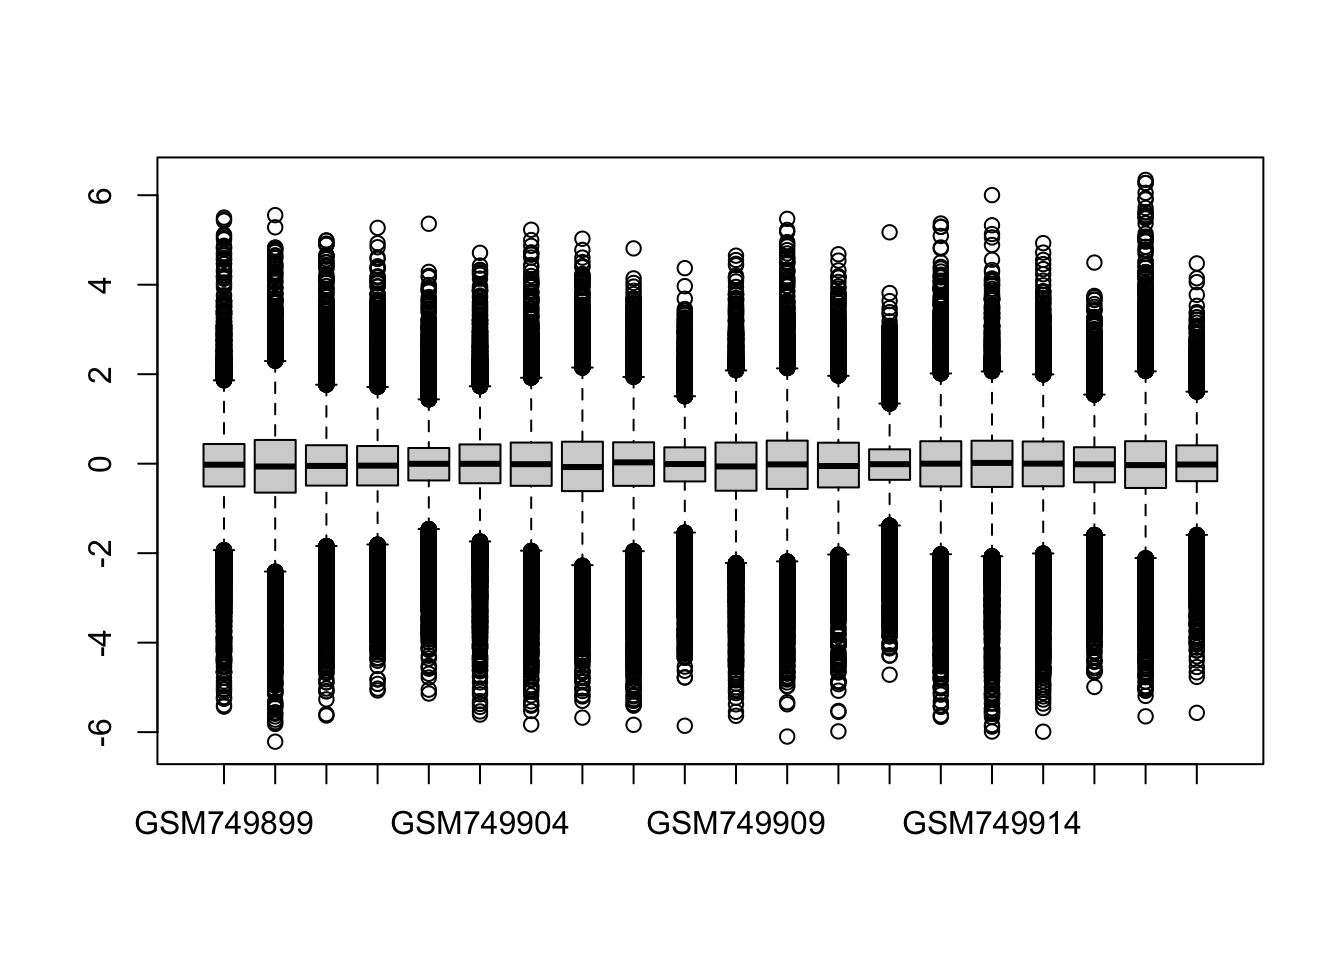
\includegraphics{20210322_REgitim_files/figure-latex/unnamed-chunk-92-1.pdf}
Gordugunuz gibi ortalamalari hemen hemen ayni olsa da (bunun sebebi verinin zaten baska bir yontemle kismen normalize edilmis olmasi), Dagilimlar farkli.

Normalizasyon icin Rda olmayan bir fonksiyon kullanacagiz, bunun icin de \texttt{preprocessCore} paketini yuklememiz gerekiyor:

\begin{Shaded}
\begin{Highlighting}[]
\NormalTok{BiocManager}\SpecialCharTok{::}\FunctionTok{install}\NormalTok{(}\StringTok{"preprocessCore"}\NormalTok{)}
\end{Highlighting}
\end{Shaded}

\begin{Shaded}
\begin{Highlighting}[]
\FunctionTok{library}\NormalTok{(preprocessCore)}
\end{Highlighting}
\end{Shaded}

Fonksiyonumuzun adi \texttt{normalize.quantiles()}

\begin{Shaded}
\begin{Highlighting}[]
\NormalTok{genexpr\_qn }\OtherTok{=} \FunctionTok{normalize.quantiles}\NormalTok{(genexpr)}
\FunctionTok{dim}\NormalTok{(genexpr\_qn)}
\end{Highlighting}
\end{Shaded}

\begin{verbatim}
## [1] 17160   269
\end{verbatim}

\begin{Shaded}
\begin{Highlighting}[]
\NormalTok{genexpr\_qn[}\DecValTok{1}\SpecialCharTok{:}\DecValTok{5}\NormalTok{,}\DecValTok{1}\SpecialCharTok{:}\DecValTok{5}\NormalTok{]}
\end{Highlighting}
\end{Shaded}

\begin{verbatim}
##            [,1]       [,2]       [,3]       [,4]       [,5]
## [1,] -0.4993920 -0.6776740 -0.7796459 -0.8040486 -0.8587960
## [2,]  1.0141904  0.8355595  0.6704056  0.5563232  0.2924776
## [3,]  1.1413791  0.9140343  1.1026208  1.4685350  1.5103426
## [4,] -0.4112961 -0.5602207 -0.6620208 -0.5704519 -0.6015157
## [5,]  1.0659865  0.8908564  0.8555507  0.8361596  0.6749602
\end{verbatim}

Gordugunuz gibi bu fonksiyon ne yazik ki satir sutun isimlerimizi sildi. Ama bunlarin ilk matrisimizle ayni oldugunu biliyoruz cunku bir subset islemi yapmadik. Eski satir-sutun isimlerimizi yeni matrisimize aktaralim:

\begin{Shaded}
\begin{Highlighting}[]
\FunctionTok{dimnames}\NormalTok{(genexpr\_qn) }\OtherTok{=} \FunctionTok{dimnames}\NormalTok{(genexpr)}
\NormalTok{genexpr\_qn[}\DecValTok{1}\SpecialCharTok{:}\DecValTok{5}\NormalTok{,}\DecValTok{1}\SpecialCharTok{:}\DecValTok{5}\NormalTok{]}
\end{Highlighting}
\end{Shaded}

\begin{verbatim}
##       GSM749899  GSM749900  GSM749901  GSM749902  GSM749903
## CTSD -0.4993920 -0.6776740 -0.7796459 -0.8040486 -0.8587960
## EEF2  1.0141904  0.8355595  0.6704056  0.5563232  0.2924776
## VIM   1.1413791  0.9140343  1.1026208  1.4685350  1.5103426
## GSN  -0.4112961 -0.5602207 -0.6620208 -0.5704519 -0.6015157
## RPN2  1.0659865  0.8908564  0.8555507  0.8361596  0.6749602
\end{verbatim}

Tekrar dagilimlara bakacak olursak:

\begin{Shaded}
\begin{Highlighting}[]
\FunctionTok{boxplot}\NormalTok{(genexpr\_qn[,}\DecValTok{1}\SpecialCharTok{:}\DecValTok{20}\NormalTok{])}
\end{Highlighting}
\end{Shaded}

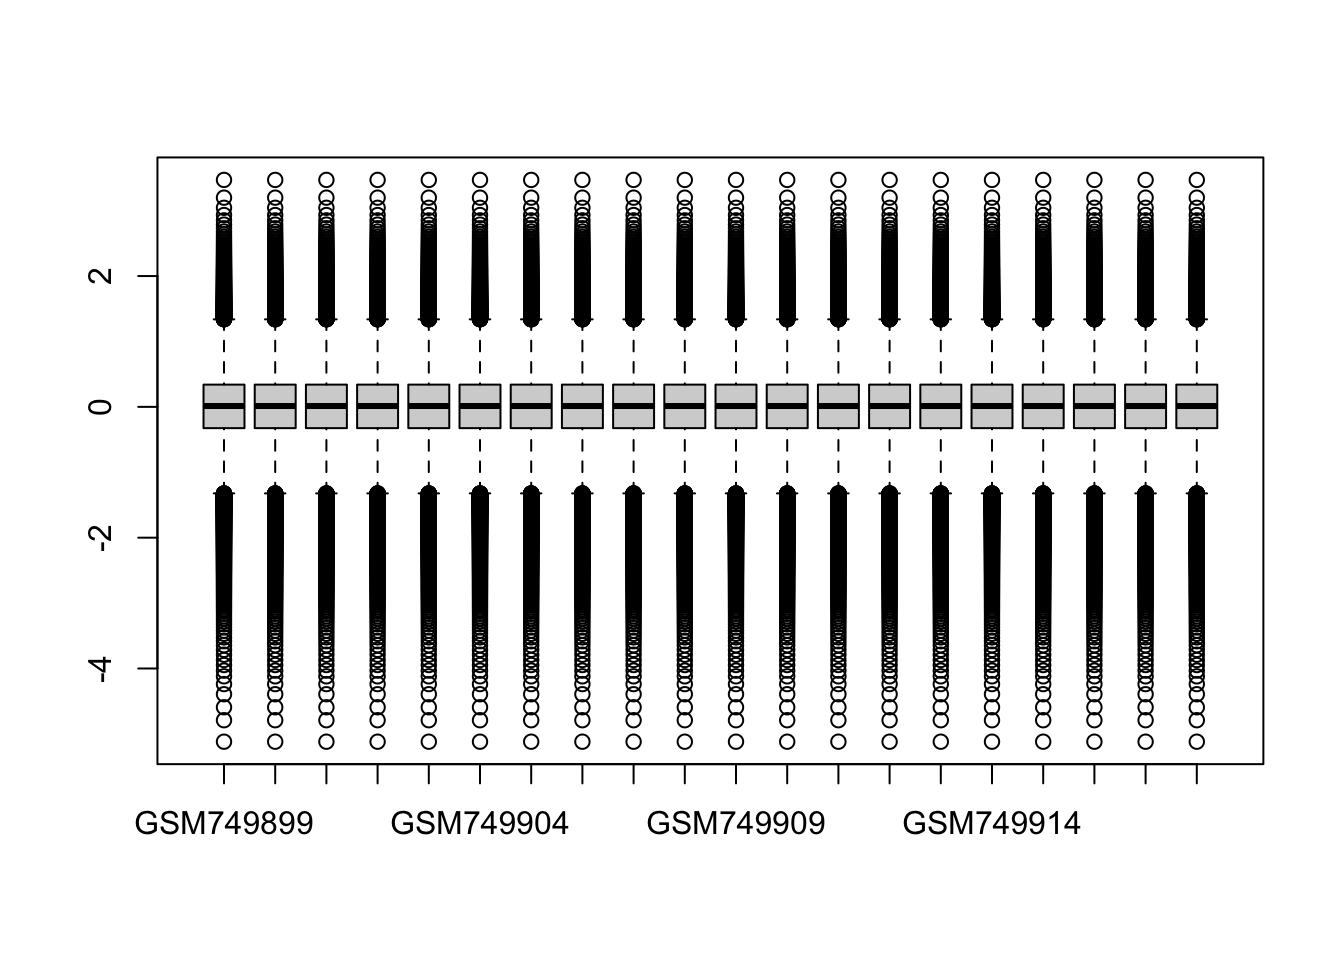
\includegraphics{20210322_REgitim_files/figure-latex/unnamed-chunk-97-1.pdf}

Gordugunuz gibi dagilimlar birebir esit oldu. Bundan sonraki asamalarda bu veriyi kullanacagiz.

\hypertarget{ornek-bilgisini-duzenleme}{%
\section{Ornek bilgisini duzenleme}\label{ornek-bilgisini-duzenleme}}

Son olarak, bir de orneklerle ilgili bilgilerin yer aldigi (yas, biyolojik cinsiyet) bir tablomuz var. Ama bu verinin de duzenlenmesi gerekiyor.

\begin{Shaded}
\begin{Highlighting}[]
\NormalTok{metadata }\OtherTok{=} \FunctionTok{read.csv}\NormalTok{(}\StringTok{\textquotesingle{}https://github.com/mdonertas/20210322\_REgitim/raw/master/data/metadata.csv\textquotesingle{}}\NormalTok{)}
\FunctionTok{head}\NormalTok{(metadata)}
\end{Highlighting}
\end{Shaded}

\begin{verbatim}
##           X    title geo_accession characteristics_ch1 characteristics_ch1.1
## 1 GSM749899 HB_18_34     GSM749899     array batch: 10     age: -0.498630137
## 2 GSM749900 HB_22_35     GSM749900     array batch: 18     age: -0.498630137
## 3 GSM749901 HB_16_29     GSM749901      array batch: 1     age: -0.498630137
## 4 GSM749902 HB_17_91     GSM749902      array batch: 8     age: -0.498630137
## 5 GSM749903 HB_18_16     GSM749903      array batch: 9     age: -0.479452055
## 6 GSM749904 HB_16_62     GSM749904      array batch: 3     age: -0.479452055
##   characteristics_ch1.2 characteristics_ch1.3        characteristics_ch1.4
## 1                Sex: F              race: AA postmortem interval (pmi): 3
## 2                Sex: F              race: AA postmortem interval (pmi): 1
## 3                Sex: M              race: AA postmortem interval (pmi): 1
## 4                Sex: M              race: AA postmortem interval (pmi): 4
## 5                Sex: M              race: AA postmortem interval (pmi): 2
## 6                Sex: M              race: AA postmortem interval (pmi): 4
##   characteristics_ch1.5           characteristics_ch1.6   characteristics_ch1.7
## 1              ph: NULL rna integrity number (rin): 9.7      smoke at death: No
## 2              ph: 6.21 rna integrity number (rin): 9.8      smoke at death: No
## 3              ph: NULL rna integrity number (rin): 9.6      smoke at death: No
## 4              ph: NULL rna integrity number (rin): 9.8      smoke at death: No
## 5              ph: NULL   rna integrity number (rin): 9 smoke at death: Unknown
## 6              ph: NULL rna integrity number (rin): 9.8      smoke at death: No
\end{verbatim}

Bu veriyi kullanarak, ayni probeset-gen eslestirmesi icin yaptigimiz gibi yas ve biyolojik cinsiyet icin birey bilgisi vektoru olusturalim:

\begin{Shaded}
\begin{Highlighting}[]
\NormalTok{yas }\OtherTok{=} \FunctionTok{setNames}\NormalTok{(metadata}\SpecialCharTok{$}\NormalTok{characteristics\_ch1}\FloatTok{.1}\NormalTok{, metadata}\SpecialCharTok{$}\NormalTok{geo\_accession)}
\FunctionTok{head}\NormalTok{(yas)}
\end{Highlighting}
\end{Shaded}

\begin{verbatim}
##           GSM749899           GSM749900           GSM749901           GSM749902 
## "age: -0.498630137" "age: -0.498630137" "age: -0.498630137" "age: -0.498630137" 
##           GSM749903           GSM749904 
## "age: -0.479452055" "age: -0.479452055"
\end{verbatim}

\begin{Shaded}
\begin{Highlighting}[]
\FunctionTok{class}\NormalTok{(yas)}
\end{Highlighting}
\end{Shaded}

\begin{verbatim}
## [1] "character"
\end{verbatim}

\begin{Shaded}
\begin{Highlighting}[]
\NormalTok{cinsiyet }\OtherTok{=} \FunctionTok{setNames}\NormalTok{(metadata}\SpecialCharTok{$}\NormalTok{characteristics\_ch1}\FloatTok{.2}\NormalTok{, metadata}\SpecialCharTok{$}\NormalTok{geo\_accession)}
\FunctionTok{head}\NormalTok{(cinsiyet)}
\end{Highlighting}
\end{Shaded}

\begin{verbatim}
## GSM749899 GSM749900 GSM749901 GSM749902 GSM749903 GSM749904 
##  "Sex: F"  "Sex: F"  "Sex: M"  "Sex: M"  "Sex: M"  "Sex: M"
\end{verbatim}

\begin{Shaded}
\begin{Highlighting}[]
\FunctionTok{class}\NormalTok{(cinsiyet)}
\end{Highlighting}
\end{Shaded}

\begin{verbatim}
## [1] "character"
\end{verbatim}

Bu veriler gordugunuz gibi karakter verileri ve formatlari pek iyi degil. Ornegin bu yas verisiyle yapabileceklerimiz sinirli cunku numerik degil. Ilk olarak basta yazan `age:' kismindan kurtulmamiz lazim ki bu yas verisini kullanabilelim. Ayni sekilde biyolojik cinsiyeti de `F' veya `M' haline, hatta daha iyisi `kadin' ve `erkek' haline getirelim.

\hypertarget{yas-verisinin-duzenlenmesi}{%
\subsection{Yas verisinin duzenlenmesi}\label{yas-verisinin-duzenlenmesi}}

Basta yazan `age:' yazisinin ortadan kaldirilmasi icin bir kac secenek var. Bunlardan en basiti \texttt{gsub} fonksiyonu. Bu fonksiyon, bir karakter vektorunde belli karakterlerin degistirilmesini saglar:

\begin{Shaded}
\begin{Highlighting}[]
\FunctionTok{gsub}\NormalTok{(}\StringTok{\textquotesingle{}range\textquotesingle{}}\NormalTok{,}\StringTok{\textquotesingle{}\textquotesingle{}}\NormalTok{,}\StringTok{\textquotesingle{}Bioinforange\textquotesingle{}}\NormalTok{)}
\end{Highlighting}
\end{Shaded}

\begin{verbatim}
## [1] "Bioinfo"
\end{verbatim}

\begin{Shaded}
\begin{Highlighting}[]
\FunctionTok{gsub}\NormalTok{(}\StringTok{\textquotesingle{}range\textquotesingle{}}\NormalTok{,}\StringTok{\textquotesingle{}conference\textquotesingle{}}\NormalTok{,}\StringTok{\textquotesingle{}Bioinforange\textquotesingle{}}\NormalTok{)}
\end{Highlighting}
\end{Shaded}

\begin{verbatim}
## [1] "Bioinfoconference"
\end{verbatim}

Bu sekilde `age:' yazisini silebiliriz:

\begin{Shaded}
\begin{Highlighting}[]
\NormalTok{yas }\OtherTok{=} \FunctionTok{gsub}\NormalTok{(}\StringTok{\textquotesingle{}age: \textquotesingle{}}\NormalTok{,}\StringTok{\textquotesingle{}\textquotesingle{}}\NormalTok{,yas)}
\FunctionTok{head}\NormalTok{(yas)}
\end{Highlighting}
\end{Shaded}

\begin{verbatim}
##      GSM749899      GSM749900      GSM749901      GSM749902      GSM749903 
## "-0.498630137" "-0.498630137" "-0.498630137" "-0.498630137" "-0.479452055" 
##      GSM749904 
## "-0.479452055"
\end{verbatim}

Ancak gordugunuz gibi, veri hala karakter. Bunu numerik yapmak icin \texttt{as.numeric()} kullaniriz:

\begin{Shaded}
\begin{Highlighting}[]
\NormalTok{yas }\OtherTok{=} \FunctionTok{setNames}\NormalTok{(}\FunctionTok{as.numeric}\NormalTok{(yas),}\FunctionTok{names}\NormalTok{(yas))}
\end{Highlighting}
\end{Shaded}

\begin{Shaded}
\begin{Highlighting}[]
\FunctionTok{hist}\NormalTok{(yas)}
\end{Highlighting}
\end{Shaded}

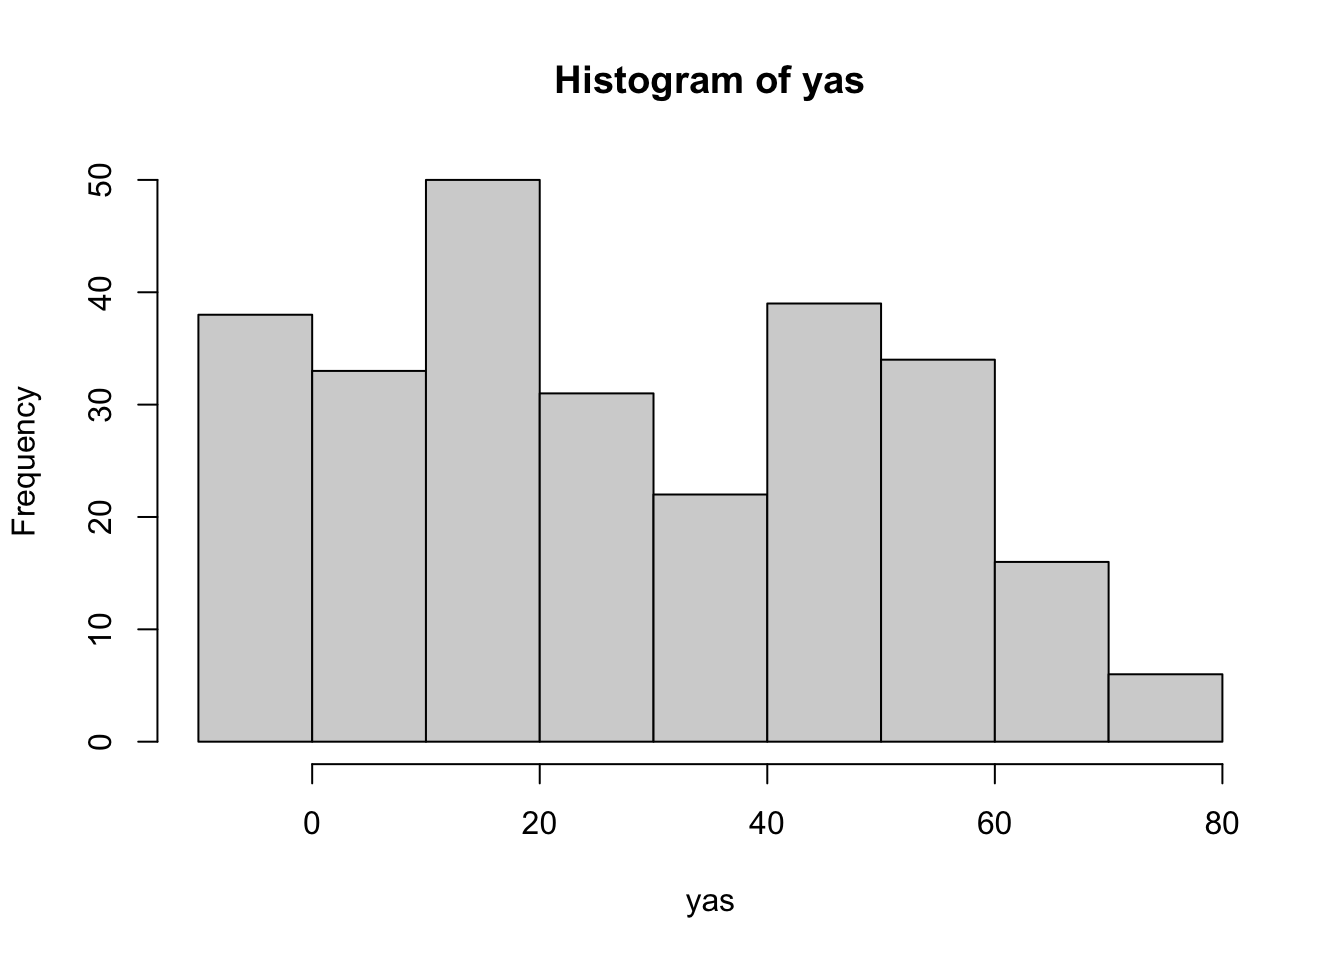
\includegraphics{20210322_REgitim_files/figure-latex/unnamed-chunk-103-1.pdf}

Daha net bir sekilde verinin ozetini gormek istersek \texttt{summary()} fonksiyonunu kullanabiliriz:

\begin{Shaded}
\begin{Highlighting}[]
\FunctionTok{summary}\NormalTok{(yas)}
\end{Highlighting}
\end{Shaded}

\begin{verbatim}
##    Min. 1st Qu.  Median    Mean 3rd Qu.    Max. 
## -0.4986  5.3452 24.2658 27.7920 46.9671 78.2274
\end{verbatim}

Dogum oncesi zamandan 78 yasina kadar bireyler var ve ortalamamiz 27.7.

\hypertarget{biyolojik-cinsiyet-verisinin-duzenlenmesi}{%
\subsection{Biyolojik cinsiyet verisinin duzenlenmesi}\label{biyolojik-cinsiyet-verisinin-duzenlenmesi}}

Bu sefer sadece 2 biyolojik cinsiyet mumkun oldugundan daha farkli bir yol izleyebiliriz. Ama oncelikle, sadece iki secenek oldugundan emin olalim.

\begin{Shaded}
\begin{Highlighting}[]
\FunctionTok{unique}\NormalTok{(cinsiyet)}
\end{Highlighting}
\end{Shaded}

\begin{verbatim}
## [1] "Sex: F" "Sex: M" "Sex: 5"
\end{verbatim}

Bir de `5' var, bu muhtemelen veri girisinde bir hata demek ama bu bireyi en azindan cinsiyet icin inceleyemeyecegimiz anlamina geliyor. Ilk olarak bu veriye sahip olan bireyi hem bu veriden hem expression verisinden hem de yas verisinden cikaralim.

\begin{Shaded}
\begin{Highlighting}[]
\NormalTok{cikart }\OtherTok{=} \FunctionTok{names}\NormalTok{(cinsiyet[(cinsiyet }\SpecialCharTok{\%in\%} \StringTok{\textquotesingle{}Sex: 5\textquotesingle{}}\NormalTok{)])}
\NormalTok{cinsiyet }\OtherTok{=}\NormalTok{ cinsiyet[}\SpecialCharTok{!}\FunctionTok{names}\NormalTok{(cinsiyet) }\SpecialCharTok{\%in\%}\NormalTok{ cikart]}
\NormalTok{yas }\OtherTok{=}\NormalTok{ yas[}\SpecialCharTok{!}\FunctionTok{names}\NormalTok{(yas) }\SpecialCharTok{\%in\%}\NormalTok{ cikart]}
\NormalTok{genexpr\_qn }\OtherTok{=}\NormalTok{ genexpr\_qn[,}\SpecialCharTok{!}\FunctionTok{colnames}\NormalTok{(genexpr\_qn) }\SpecialCharTok{\%in\%}\NormalTok{ cikart]}
\end{Highlighting}
\end{Shaded}

Ayni probeset-gen eslesmesi yapmak icin kullandigimiz gibi bir vektor olusturalim:

\begin{Shaded}
\begin{Highlighting}[]
\NormalTok{cinsiyetMap }\OtherTok{=} \FunctionTok{setNames}\NormalTok{(}\FunctionTok{c}\NormalTok{(}\StringTok{\textquotesingle{}Kadin\textquotesingle{}}\NormalTok{,}\StringTok{\textquotesingle{}Erkek\textquotesingle{}}\NormalTok{),}\FunctionTok{c}\NormalTok{(}\StringTok{\textquotesingle{}Sex: F\textquotesingle{}}\NormalTok{,}\StringTok{\textquotesingle{}Sex: M\textquotesingle{}}\NormalTok{))}
\NormalTok{cinsiyet }\OtherTok{=} \FunctionTok{setNames}\NormalTok{(cinsiyetMap[cinsiyet],}\FunctionTok{names}\NormalTok{(cinsiyet))}
\FunctionTok{head}\NormalTok{(cinsiyet)}
\end{Highlighting}
\end{Shaded}

\begin{verbatim}
## GSM749899 GSM749900 GSM749901 GSM749902 GSM749903 GSM749904 
##   "Kadin"   "Kadin"   "Erkek"   "Erkek"   "Erkek"   "Erkek"
\end{verbatim}

Kac kadin kac erkek bireyin olduguna bakmak icin \texttt{table()} fonksiyonunu kullanabiliriz:

\begin{Shaded}
\begin{Highlighting}[]
\FunctionTok{table}\NormalTok{(cinsiyet)}
\end{Highlighting}
\end{Shaded}

\begin{verbatim}
## cinsiyet
## Erkek Kadin 
##   177    91
\end{verbatim}

\hypertarget{temel-bilesenler-analizi}{%
\chapter{Temel bilesenler analizi}\label{temel-bilesenler-analizi}}

\begin{Shaded}
\begin{Highlighting}[]
\NormalTok{tba }\OtherTok{=} \FunctionTok{prcomp}\NormalTok{(}\FunctionTok{t}\NormalTok{(genexpr\_qn), }\AttributeTok{scale. =}\NormalTok{ T)}
\end{Highlighting}
\end{Shaded}

\begin{Shaded}
\begin{Highlighting}[]
\NormalTok{renkler }\OtherTok{=} \FunctionTok{colorRampPalette}\NormalTok{(}\FunctionTok{c}\NormalTok{(}\StringTok{\textquotesingle{}pink\textquotesingle{}}\NormalTok{,}\StringTok{\textquotesingle{}darkred\textquotesingle{}}\NormalTok{))(}\FunctionTok{length}\NormalTok{(yas))}
\NormalTok{renkler\_sirali }\OtherTok{=}\NormalTok{ renkler[}\FunctionTok{rank}\NormalTok{(yas[}\FunctionTok{rownames}\NormalTok{(tba}\SpecialCharTok{$}\NormalTok{x)], }\AttributeTok{ties.method =} \StringTok{\textquotesingle{}min\textquotesingle{}}\NormalTok{)]}
\FunctionTok{plot}\NormalTok{(}\AttributeTok{x =}\NormalTok{ tba}\SpecialCharTok{$}\NormalTok{x[,}\DecValTok{1}\NormalTok{], }\AttributeTok{y =}\NormalTok{ tba}\SpecialCharTok{$}\NormalTok{x[,}\DecValTok{2}\NormalTok{], }\AttributeTok{pch =} \DecValTok{19}\NormalTok{, }\AttributeTok{cex =} \FloatTok{0.5}\NormalTok{, }\AttributeTok{col =}\NormalTok{ renkler\_sirali, }
     \AttributeTok{xlab =} \StringTok{\textquotesingle{}PC1\textquotesingle{}}\NormalTok{, }\AttributeTok{ylab =} \StringTok{\textquotesingle{}PC2\textquotesingle{}}\NormalTok{)}
\end{Highlighting}
\end{Shaded}

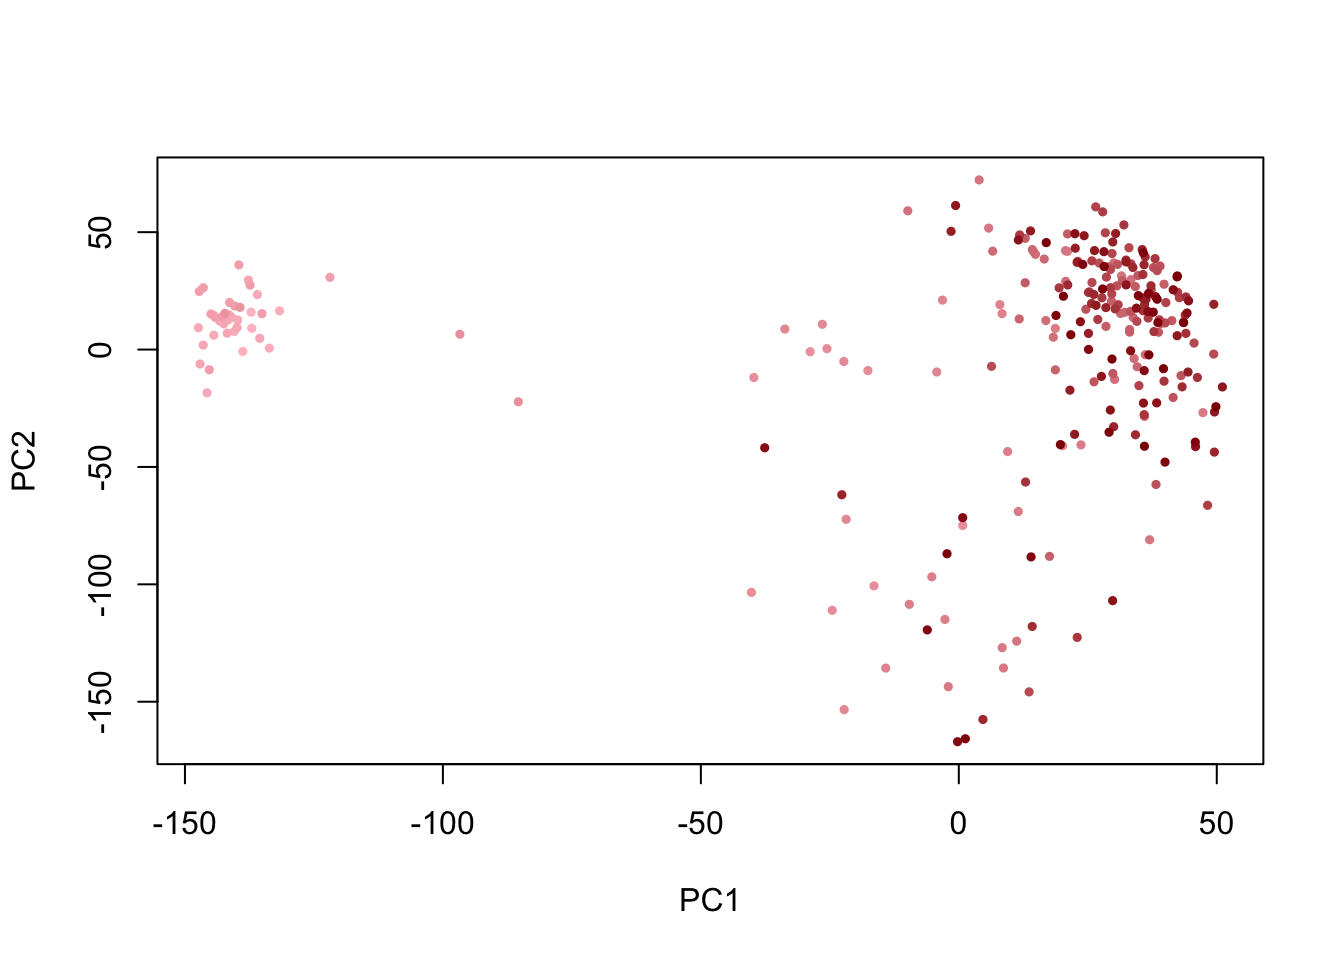
\includegraphics{20210322_REgitim_files/figure-latex/unnamed-chunk-110-1.pdf}

Ayni figuru ggplot ile yapabiliriz. Ancak bunun icin bir kac \texttt{tidyverse}de yer alan paketlerden bir kac fonksiyon kullanarak veriyi sekillendirmem gerekiyor:

\begin{Shaded}
\begin{Highlighting}[]
\FunctionTok{library}\NormalTok{(tidyverse)}
\NormalTok{pcadat }\OtherTok{=} \FunctionTok{as.data.frame}\NormalTok{(tba}\SpecialCharTok{$}\NormalTok{x[,}\DecValTok{1}\SpecialCharTok{:}\DecValTok{2}\NormalTok{]) }\SpecialCharTok{\%\textgreater{}\%}
  \FunctionTok{mutate}\NormalTok{(}\AttributeTok{sample =} \FunctionTok{rownames}\NormalTok{(tba}\SpecialCharTok{$}\NormalTok{x)) }\SpecialCharTok{\%\textgreater{}\%}
  \FunctionTok{mutate}\NormalTok{(}\AttributeTok{yas =}\NormalTok{ yas[sample],}
         \AttributeTok{cinsiyet =}\NormalTok{ cinsiyet[sample])}
\FunctionTok{head}\NormalTok{(pcadat)}
\end{Highlighting}
\end{Shaded}

\begin{verbatim}
##         PC1        PC2    sample        yas cinsiyet
## 1 -138.7854 -0.7978871 GSM749899 -0.4986301    Kadin
## 2 -137.1751 15.9124596 GSM749900 -0.4986301    Kadin
## 3 -142.7689 13.8844269 GSM749901 -0.4986301    Erkek
## 4 -137.0419  9.0980053 GSM749902 -0.4986301    Erkek
## 5 -133.6389  0.6007799 GSM749903 -0.4794521    Erkek
## 6 -131.6583 16.4774424 GSM749904 -0.4794521    Erkek
\end{verbatim}

\begin{Shaded}
\begin{Highlighting}[]
\FunctionTok{ggplot}\NormalTok{(pcadat, }\FunctionTok{aes}\NormalTok{(}\AttributeTok{x =}\NormalTok{ PC1, }\AttributeTok{y =}\NormalTok{ PC2, }\AttributeTok{color =}\NormalTok{ yas, }\AttributeTok{shape =}\NormalTok{ cinsiyet)) }\SpecialCharTok{+}
  \FunctionTok{geom\_point}\NormalTok{(}\AttributeTok{size =} \DecValTok{3}\NormalTok{) }\SpecialCharTok{+}
  \FunctionTok{scale\_color\_gradient}\NormalTok{(}\AttributeTok{low =} \StringTok{\textquotesingle{}pink\textquotesingle{}}\NormalTok{, }\AttributeTok{high =} \StringTok{\textquotesingle{}darkred\textquotesingle{}}\NormalTok{) }\SpecialCharTok{+}
  \FunctionTok{theme\_bw}\NormalTok{()}
\end{Highlighting}
\end{Shaded}

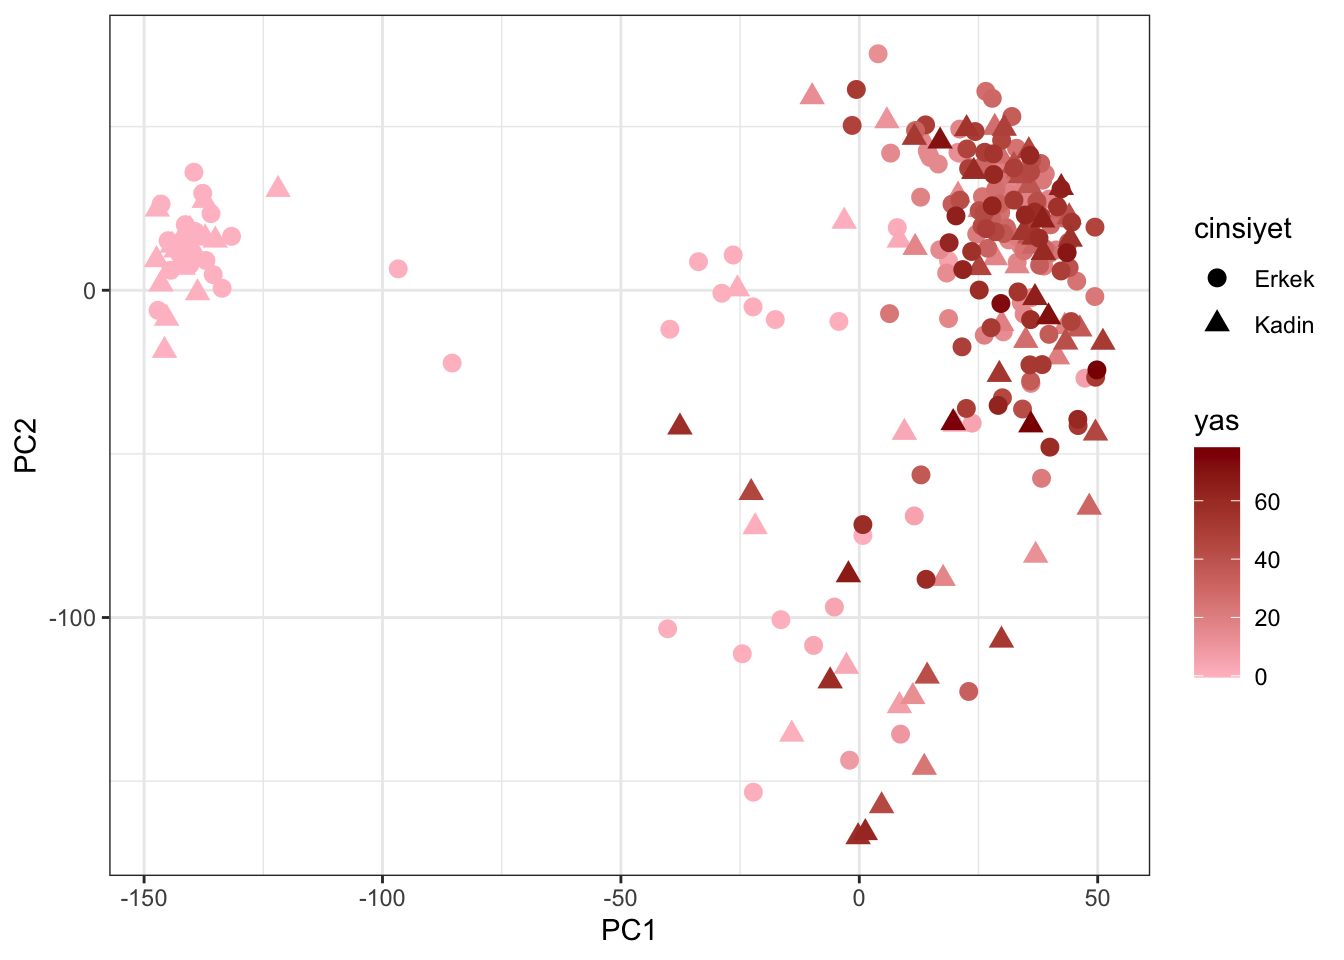
\includegraphics{20210322_REgitim_files/figure-latex/unnamed-chunk-111-1.pdf}

\hypertarget{yasla-degisim-analizi}{%
\chapter{Yasla degisim analizi}\label{yasla-degisim-analizi}}

Diyelim ki sadece dogum sonrasi donemde 20 sonrasi yasta yasla degisen genlerle ilgileniyoruz. Bunun icin ilk olarak veriyi subset etmeliyiz. Yas'in 20den buyuk oldugu bireyleri almaliyiz:

\begin{Shaded}
\begin{Highlighting}[]
\NormalTok{subsamp }\OtherTok{=} \FunctionTok{names}\NormalTok{(}\FunctionTok{which}\NormalTok{(yas}\SpecialCharTok{\textgreater{}=}\DecValTok{20}\NormalTok{))}
\NormalTok{subexp }\OtherTok{=}\NormalTok{ genexpr\_qn[,subsamp]}
\NormalTok{subyas }\OtherTok{=}\NormalTok{ yas[subsamp]}
\end{Highlighting}
\end{Shaded}

\begin{Shaded}
\begin{Highlighting}[]
\NormalTok{yasladegisim }\OtherTok{=} \FunctionTok{apply}\NormalTok{(subexp, }\DecValTok{1}\NormalTok{, }\ControlFlowTok{function}\NormalTok{(x)\{}
\NormalTok{  co }\OtherTok{=} \FunctionTok{cor.test}\NormalTok{(x, subyas[}\FunctionTok{colnames}\NormalTok{(subexp)], }\AttributeTok{method =} \StringTok{\textquotesingle{}spearman\textquotesingle{}}\NormalTok{)}
  \FunctionTok{c}\NormalTok{(co}\SpecialCharTok{$}\NormalTok{est, co}\SpecialCharTok{$}\NormalTok{p.val)}
\NormalTok{\})}
\end{Highlighting}
\end{Shaded}

\begin{Shaded}
\begin{Highlighting}[]
\FunctionTok{dim}\NormalTok{(yasladegisim)}
\end{Highlighting}
\end{Shaded}

\begin{verbatim}
## [1]     2 17160
\end{verbatim}

\begin{Shaded}
\begin{Highlighting}[]
\NormalTok{yasladegisim }\OtherTok{=} \FunctionTok{t}\NormalTok{(yasladegisim)}
\FunctionTok{head}\NormalTok{(yasladegisim)}
\end{Highlighting}
\end{Shaded}

\begin{verbatim}
##                rho             
## CTSD   -0.03253336 0.6956624723
## EEF2   -0.12309924 0.1374343793
## VIM     0.28300932 0.0005395356
## GSN     0.11697104 0.1581010511
## RPN2   -0.22977129 0.0052073498
## POLR2A  0.01173037 0.8878589579
\end{verbatim}

\begin{Shaded}
\begin{Highlighting}[]
\FunctionTok{colnames}\NormalTok{(yasladegisim) }\OtherTok{=} \FunctionTok{c}\NormalTok{(}\StringTok{\textquotesingle{}rho\textquotesingle{}}\NormalTok{,}\StringTok{\textquotesingle{}p\textquotesingle{}}\NormalTok{)}
\NormalTok{yasladegisim }\OtherTok{=} \FunctionTok{cbind}\NormalTok{(yasladegisim, }\FunctionTok{p.adjust}\NormalTok{(yasladegisim[,}\StringTok{\textquotesingle{}p\textquotesingle{}}\NormalTok{], }\AttributeTok{method=} \StringTok{\textquotesingle{}fdr\textquotesingle{}}\NormalTok{))}
\end{Highlighting}
\end{Shaded}

Hangi genler yasla istatistiksel olarak anlamli degisim gosteriyor?

\begin{Shaded}
\begin{Highlighting}[]
\NormalTok{anlamli }\OtherTok{=} \FunctionTok{names}\NormalTok{(}\FunctionTok{which}\NormalTok{(yasladegisim[,}\DecValTok{3}\NormalTok{]}\SpecialCharTok{\textless{}=}\FloatTok{0.05}\NormalTok{))}
\FunctionTok{table}\NormalTok{(yasladegisim[}\FunctionTok{rownames}\NormalTok{(yasladegisim)}\SpecialCharTok{\%in\%}\NormalTok{anlamli,}\DecValTok{1}\NormalTok{]}\SpecialCharTok{\textgreater{}=}\DecValTok{0}\NormalTok{)}
\end{Highlighting}
\end{Shaded}

\begin{verbatim}
## 
## FALSE  TRUE 
##  1538  1418
\end{verbatim}

Bunlardan 1419 tanesi artis yonunde anlamli degisim gosteriyor, 1538 tanesi ise dusus. Bunlardan en cok artis gostereni secip gorsellestirelim:

\begin{Shaded}
\begin{Highlighting}[]
\NormalTok{maxartis }\OtherTok{=} \FunctionTok{names}\NormalTok{(}\FunctionTok{which.max}\NormalTok{(yasladegisim[,}\DecValTok{1}\NormalTok{]))}
\NormalTok{yasladegisim[maxartis,]}
\end{Highlighting}
\end{Shaded}

\begin{verbatim}
##          rho            p              
## 6.980232e-01 8.761466e-23 1.002312e-19
\end{verbatim}

\begin{Shaded}
\begin{Highlighting}[]
\FunctionTok{plot}\NormalTok{(}\AttributeTok{x =}\NormalTok{ subyas, }\AttributeTok{y =}\NormalTok{ subexp[maxartis,], }\AttributeTok{pch =} \DecValTok{19}\NormalTok{, }\AttributeTok{cex =} \FloatTok{0.5}\NormalTok{, }\AttributeTok{xlab=}\StringTok{\textquotesingle{}Yas\textquotesingle{}}\NormalTok{,}
     \AttributeTok{ylab =} \StringTok{\textquotesingle{}Gen ifadesi\textquotesingle{}}\NormalTok{, }\AttributeTok{main =}\NormalTok{ maxartis)}
\FunctionTok{abline}\NormalTok{(}\FunctionTok{lm}\NormalTok{(subexp[maxartis,]}\SpecialCharTok{\textasciitilde{}}\NormalTok{subyas), }\AttributeTok{col =} \StringTok{\textquotesingle{}darkred\textquotesingle{}}\NormalTok{,}\AttributeTok{cex =} \DecValTok{2}\NormalTok{)}
\end{Highlighting}
\end{Shaded}

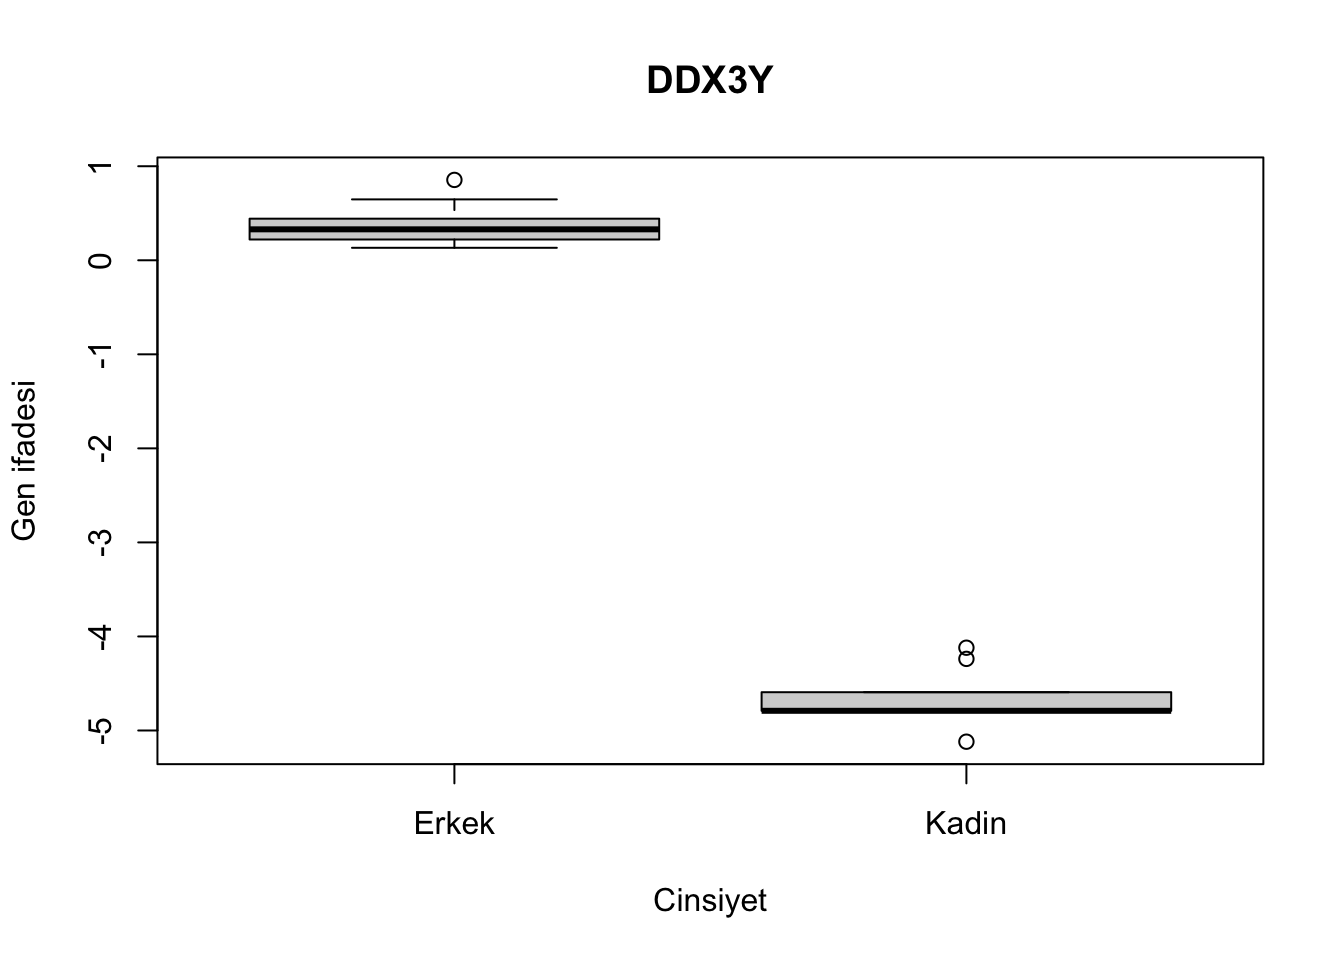
\includegraphics{20210322_REgitim_files/figure-latex/unnamed-chunk-117-1.pdf}

\begin{Shaded}
\begin{Highlighting}[]
\FunctionTok{pdf}\NormalTok{(}\StringTok{\textquotesingle{}./yasladegisim.pdf\textquotesingle{}}\NormalTok{)}
\FunctionTok{plot}\NormalTok{(}\AttributeTok{x =}\NormalTok{ subyas, }\AttributeTok{y =}\NormalTok{ subexp[maxartis,], }\AttributeTok{pch =} \DecValTok{19}\NormalTok{, }\AttributeTok{cex =} \FloatTok{0.5}\NormalTok{, }\AttributeTok{xlab=}\StringTok{\textquotesingle{}Yas\textquotesingle{}}\NormalTok{,}
     \AttributeTok{ylab =} \StringTok{\textquotesingle{}Gen ifadesi\textquotesingle{}}\NormalTok{, }\AttributeTok{main =}\NormalTok{ maxartis)}
\FunctionTok{abline}\NormalTok{(}\FunctionTok{lm}\NormalTok{(subexp[maxartis,]}\SpecialCharTok{\textasciitilde{}}\NormalTok{subyas), }\AttributeTok{col =} \StringTok{\textquotesingle{}darkred\textquotesingle{}}\NormalTok{,}\AttributeTok{cex =} \DecValTok{2}\NormalTok{)}
\FunctionTok{dev.off}\NormalTok{()}
\end{Highlighting}
\end{Shaded}

\begin{verbatim}
## pdf 
##   2
\end{verbatim}

\begin{Shaded}
\begin{Highlighting}[]
\FunctionTok{write.csv}\NormalTok{(}\AttributeTok{x =}\NormalTok{ yasladegisim, }\AttributeTok{file =} \StringTok{\textquotesingle{}./yasladegisim.csv\textquotesingle{}}\NormalTok{,}\AttributeTok{quote =}\NormalTok{ F,}
          \AttributeTok{row.names =}\NormalTok{ T)}
\end{Highlighting}
\end{Shaded}

Ayni figuru ggplot ile cizelim:

\begin{Shaded}
\begin{Highlighting}[]
\NormalTok{mydat }\OtherTok{=} \FunctionTok{data.frame}\NormalTok{(}\AttributeTok{expression =}\NormalTok{ subexp[maxartis,], }\AttributeTok{sample  =} \FunctionTok{colnames}\NormalTok{(subexp), }
                   \AttributeTok{yas =}\NormalTok{ subyas[}\FunctionTok{colnames}\NormalTok{(subexp)],}\AttributeTok{cinsiyet =}\NormalTok{ cinsiyet[}\FunctionTok{colnames}\NormalTok{(subexp)])}
\FunctionTok{ggplot}\NormalTok{(mydat, }\FunctionTok{aes}\NormalTok{(}\AttributeTok{x =}\NormalTok{ yas, }\AttributeTok{y =}\NormalTok{ expression)) }\SpecialCharTok{+}
  \FunctionTok{geom\_point}\NormalTok{(}\FunctionTok{aes}\NormalTok{(}\AttributeTok{color =}\NormalTok{ cinsiyet)) }\SpecialCharTok{+} 
  \FunctionTok{geom\_smooth}\NormalTok{(}\AttributeTok{method =} \StringTok{\textquotesingle{}lm\textquotesingle{}}\NormalTok{, }\AttributeTok{color =} \StringTok{\textquotesingle{}midnightblue\textquotesingle{}}\NormalTok{) }\SpecialCharTok{+}
  \FunctionTok{scale\_color\_brewer}\NormalTok{(}\AttributeTok{type =} \StringTok{\textquotesingle{}qual\textquotesingle{}}\NormalTok{, }\AttributeTok{palette =} \DecValTok{6}\NormalTok{) }\SpecialCharTok{+}
  \FunctionTok{theme\_bw}\NormalTok{()}
\end{Highlighting}
\end{Shaded}

\begin{verbatim}
## `geom_smooth()` using formula 'y ~ x'
\end{verbatim}

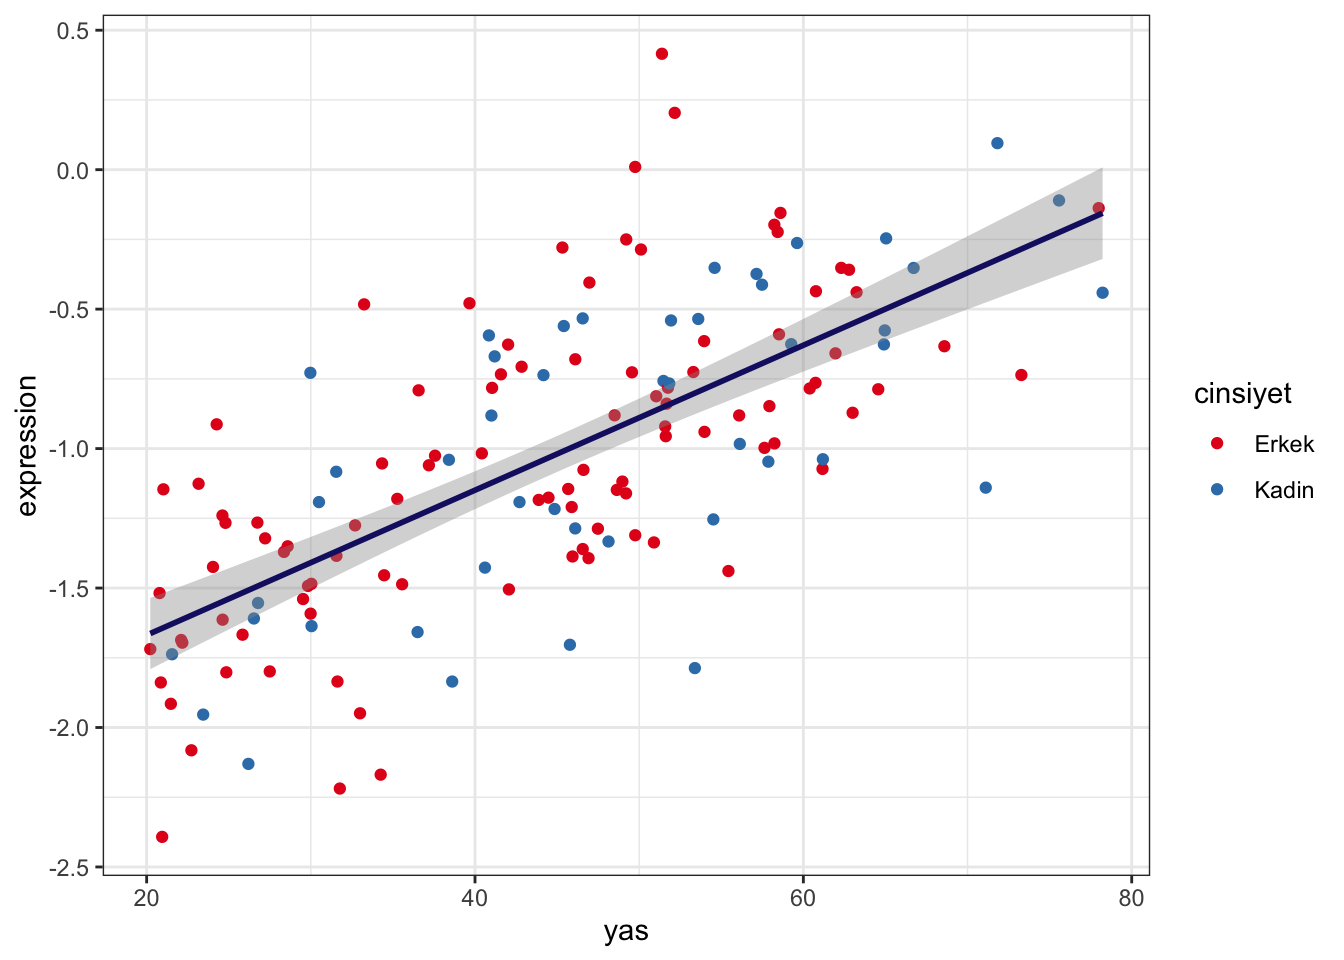
\includegraphics{20210322_REgitim_files/figure-latex/unnamed-chunk-120-1.pdf}

\hypertarget{biyolojik-cinsiyete-gore-farklilik-gosteren-gen-analizi}{%
\chapter{Biyolojik cinsiyete gore farklilik gosteren gen analizi}\label{biyolojik-cinsiyete-gore-farklilik-gosteren-gen-analizi}}

Diyelim ki sadece dogum sonrasi donemde 20 sonrasi ve 40 yas oncesi yasta kadin ve erkekler arasinda farkli gen ifadesi gosteren genlerle ilgileniyoruz.

\begin{Shaded}
\begin{Highlighting}[]
\NormalTok{subsamp }\OtherTok{=} \FunctionTok{names}\NormalTok{(}\FunctionTok{which}\NormalTok{(yas}\SpecialCharTok{\textgreater{}=}\DecValTok{20} \SpecialCharTok{\&}\NormalTok{ yas}\SpecialCharTok{\textless{}}\DecValTok{40}\NormalTok{))}
\NormalTok{subexp }\OtherTok{=}\NormalTok{ genexpr\_qn[,subsamp]}
\NormalTok{subyas }\OtherTok{=}\NormalTok{ yas[subsamp]}
\NormalTok{subcins }\OtherTok{=}\NormalTok{ cinsiyet[subsamp]}
\FunctionTok{table}\NormalTok{(subcins)}
\end{Highlighting}
\end{Shaded}

\begin{verbatim}
## subcins
## Erkek Kadin 
##    41    12
\end{verbatim}

Kadin ve erkek sayisindaki fark cok fazla. Hem erkek hem de kadinlarin icinden rastegele 10ar birey secip analiz yapalim (- rastgele secim yapmayi gostermek icin!).

\begin{Shaded}
\begin{Highlighting}[]
\NormalTok{erkek }\OtherTok{=} \FunctionTok{sample}\NormalTok{(}\FunctionTok{names}\NormalTok{(}\FunctionTok{which}\NormalTok{(subcins }\SpecialCharTok{==} \StringTok{\textquotesingle{}Erkek\textquotesingle{}}\NormalTok{)),}\DecValTok{10}\NormalTok{,}\AttributeTok{replace =}\NormalTok{ F)}
\NormalTok{kadin }\OtherTok{=} \FunctionTok{sample}\NormalTok{(}\FunctionTok{names}\NormalTok{(}\FunctionTok{which}\NormalTok{(subcins }\SpecialCharTok{==} \StringTok{\textquotesingle{}Kadin\textquotesingle{}}\NormalTok{)),}\DecValTok{10}\NormalTok{,}\AttributeTok{replace =}\NormalTok{ F)}
\NormalTok{subsamp }\OtherTok{=} \FunctionTok{c}\NormalTok{(erkek,kadin)}
\NormalTok{subexp }\OtherTok{=}\NormalTok{ genexpr\_qn[,subsamp]}
\NormalTok{subyas }\OtherTok{=}\NormalTok{ yas[subsamp]}
\NormalTok{subcins }\OtherTok{=}\NormalTok{ cinsiyet[subsamp]}
\FunctionTok{table}\NormalTok{(subcins)}
\end{Highlighting}
\end{Shaded}

\begin{verbatim}
## subcins
## Erkek Kadin 
##    10    10
\end{verbatim}

\begin{Shaded}
\begin{Highlighting}[]
\NormalTok{cinsiyetfark }\OtherTok{=} \FunctionTok{apply}\NormalTok{(subexp, }\DecValTok{1}\NormalTok{, }\ControlFlowTok{function}\NormalTok{(x)\{}
\NormalTok{  tres }\OtherTok{=} \FunctionTok{t.test}\NormalTok{(x}\SpecialCharTok{\textasciitilde{}}\NormalTok{subcins)}
  \FunctionTok{c}\NormalTok{(tres}\SpecialCharTok{$}\NormalTok{statistic, tres}\SpecialCharTok{$}\NormalTok{p.value)}
\NormalTok{\})}
\end{Highlighting}
\end{Shaded}

\begin{Shaded}
\begin{Highlighting}[]
\FunctionTok{dim}\NormalTok{(cinsiyetfark)}
\end{Highlighting}
\end{Shaded}

\begin{verbatim}
## [1]     2 17160
\end{verbatim}

\begin{Shaded}
\begin{Highlighting}[]
\NormalTok{cinsiyetfark }\OtherTok{=} \FunctionTok{t}\NormalTok{(cinsiyetfark)}
\FunctionTok{head}\NormalTok{(cinsiyetfark)}
\end{Highlighting}
\end{Shaded}

\begin{verbatim}
##                t           
## CTSD   0.5578246 0.58411736
## EEF2   1.4946400 0.15355839
## VIM    1.3385760 0.19762426
## GSN    0.6706439 0.51180855
## RPN2   1.8386448 0.08256833
## POLR2A 1.0043784 0.32906296
\end{verbatim}

\begin{Shaded}
\begin{Highlighting}[]
\FunctionTok{colnames}\NormalTok{(cinsiyetfark) }\OtherTok{=} \FunctionTok{c}\NormalTok{(}\StringTok{\textquotesingle{}t\textquotesingle{}}\NormalTok{,}\StringTok{\textquotesingle{}p\textquotesingle{}}\NormalTok{)}
\NormalTok{cinsiyetfark }\OtherTok{=} \FunctionTok{cbind}\NormalTok{(cinsiyetfark,}\FunctionTok{p.adjust}\NormalTok{(cinsiyetfark[,}\StringTok{\textquotesingle{}p\textquotesingle{}}\NormalTok{],}\AttributeTok{method=} \StringTok{\textquotesingle{}fdr\textquotesingle{}}\NormalTok{))}
\end{Highlighting}
\end{Shaded}

Hangi genler yasla istatistiksel olarak anlamli degisim gosteriyor?

\begin{Shaded}
\begin{Highlighting}[]
\NormalTok{anlamli }\OtherTok{=} \FunctionTok{names}\NormalTok{(}\FunctionTok{which}\NormalTok{(cinsiyetfark[,}\DecValTok{3}\NormalTok{]}\SpecialCharTok{\textless{}=}\FloatTok{0.05}\NormalTok{))}
\FunctionTok{length}\NormalTok{(anlamli)}
\end{Highlighting}
\end{Shaded}

\begin{verbatim}
## [1] 11
\end{verbatim}

Sadece 12 gen anlamli fark gostermis.

\begin{Shaded}
\begin{Highlighting}[]
\NormalTok{maxfark }\OtherTok{=} \FunctionTok{names}\NormalTok{(}\FunctionTok{which.max}\NormalTok{(}\FunctionTok{abs}\NormalTok{(cinsiyetfark[,}\DecValTok{1}\NormalTok{])))}
\NormalTok{cinsiyetfark[maxfark,]}
\end{Highlighting}
\end{Shaded}

\begin{verbatim}
##            t            p              
## 4.130682e+01 1.286897e-17 1.104158e-13
\end{verbatim}

\begin{Shaded}
\begin{Highlighting}[]
\FunctionTok{boxplot}\NormalTok{(subexp[maxfark,]}\SpecialCharTok{\textasciitilde{}}\NormalTok{subcins, }\AttributeTok{ylab =} \StringTok{\textquotesingle{}Gen ifadesi\textquotesingle{}}\NormalTok{, }\AttributeTok{main =}\NormalTok{ maxfark, }
        \AttributeTok{xlab =} \StringTok{\textquotesingle{}Cinsiyet\textquotesingle{}}\NormalTok{)}
\end{Highlighting}
\end{Shaded}

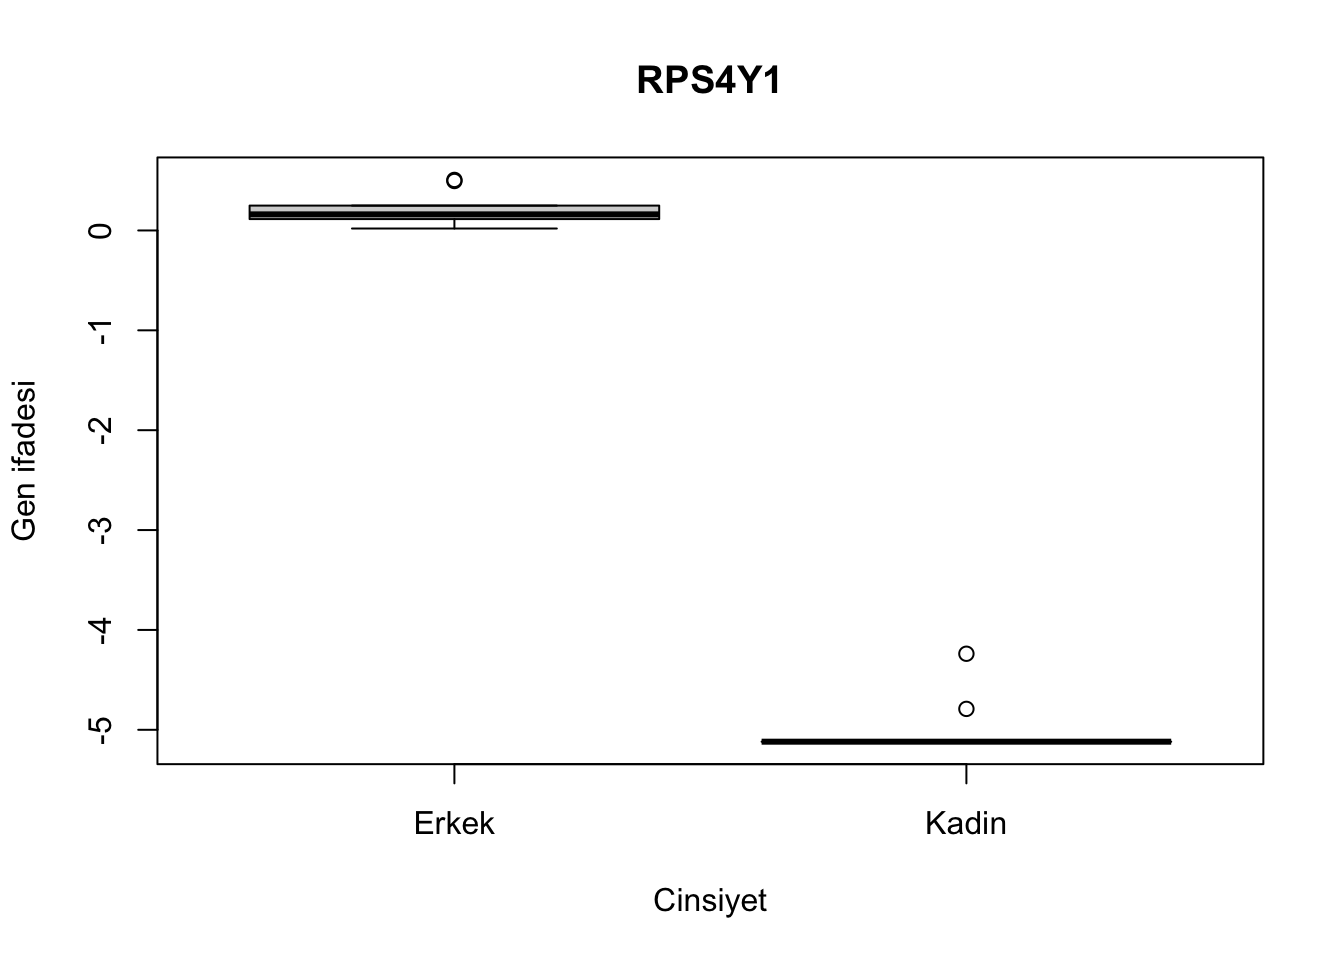
\includegraphics{20210322_REgitim_files/figure-latex/unnamed-chunk-127-1.pdf}

Figuru kaydetmek icin:

\begin{Shaded}
\begin{Highlighting}[]
\FunctionTok{pdf}\NormalTok{(}\StringTok{\textquotesingle{}./cinsiyetfark.pdf\textquotesingle{}}\NormalTok{)}
\FunctionTok{boxplot}\NormalTok{(subexp[maxfark,]}\SpecialCharTok{\textasciitilde{}}\NormalTok{subcins, }\AttributeTok{ylab =} \StringTok{\textquotesingle{}Gen ifadesi\textquotesingle{}}\NormalTok{, }\AttributeTok{main =}\NormalTok{ maxfark, }
        \AttributeTok{xlab =} \StringTok{\textquotesingle{}Cinsiyet\textquotesingle{}}\NormalTok{)}
\FunctionTok{dev.off}\NormalTok{()}
\end{Highlighting}
\end{Shaded}

\begin{verbatim}
## pdf 
##   2
\end{verbatim}

Ayni figuru ggplotta cizelim:

\begin{Shaded}
\begin{Highlighting}[]
\NormalTok{mydat }\OtherTok{=} \FunctionTok{data.frame}\NormalTok{(}\AttributeTok{expression =}\NormalTok{ subexp[maxfark,], }
                   \AttributeTok{cinsiyet =}\NormalTok{ subcins[}\FunctionTok{colnames}\NormalTok{(subexp)], }
                   \AttributeTok{yas =}\NormalTok{ yas[}\FunctionTok{colnames}\NormalTok{(subexp)])}
\FunctionTok{ggplot}\NormalTok{(mydat, }\FunctionTok{aes}\NormalTok{(}\AttributeTok{x =}\NormalTok{ cinsiyet, }\AttributeTok{y =}\NormalTok{ expression)) }\SpecialCharTok{+}
  \FunctionTok{geom\_violin}\NormalTok{(}\FunctionTok{aes}\NormalTok{(}\AttributeTok{fill =}\NormalTok{ cinsiyet), }\AttributeTok{alpha =} \FloatTok{0.5}\NormalTok{) }\SpecialCharTok{+}
  \FunctionTok{scale\_fill\_brewer}\NormalTok{(}\AttributeTok{type=}\StringTok{\textquotesingle{}qual\textquotesingle{}}\NormalTok{, }\AttributeTok{palette =} \DecValTok{6}\NormalTok{)}\SpecialCharTok{+}
  \FunctionTok{geom\_boxplot}\NormalTok{(}\AttributeTok{outlier.shape =} \ConstantTok{NA}\NormalTok{, }\AttributeTok{width =} \FloatTok{0.1}\NormalTok{) }\SpecialCharTok{+}
  \FunctionTok{theme\_bw}\NormalTok{()}
\end{Highlighting}
\end{Shaded}

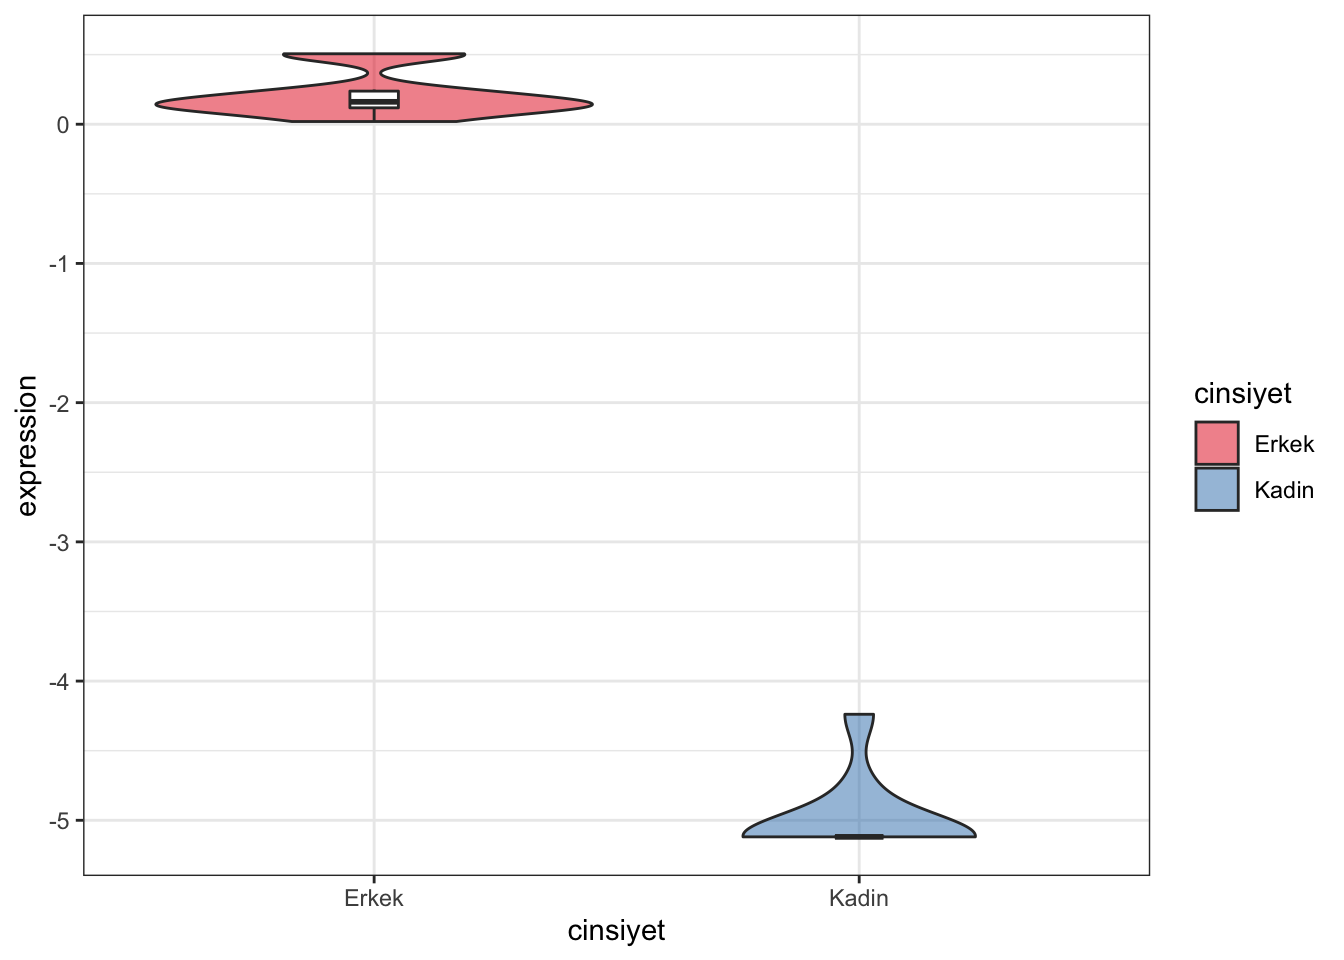
\includegraphics{20210322_REgitim_files/figure-latex/unnamed-chunk-129-1.pdf}

\hypertarget{kaynak-onerileri}{%
\chapter{Kaynak onerileri}\label{kaynak-onerileri}}

\hypertarget{online-ders}{%
\section{Online ders}\label{online-ders}}

\begin{itemize}
\item
  R ve veri bilimine giris: \url{https://www.edx.org/professional-certificate/harvardx-data-science}
\item
  R ve yasam bilimlerinde veri analizi: \url{https://www.edx.org/professional-certificate/harvardx-data-analysis-for-life-sciences}
\item
  Rda genomik analiz: \url{https://www.edx.org/professional-certificate/harvardx-data-analysis-for-genomics}
\item
  R programlama: \url{https://www.coursera.org/learn/r-programming}
\item
  Coursera Data Science Specialization icinde \textasciitilde10 ders var: \url{https://www.coursera.org/specializations/jhu-data-science}
\end{itemize}

\hypertarget{kitaplar}{%
\section{Kitaplar}\label{kitaplar}}

\begin{itemize}
\item
  R Programming for Data Science: \url{https://leanpub.com/rprogramming}
\item
  Data Analysis for the Life Sciences: \url{https://leanpub.com/dataanalysisforthelifesciences}
\item
  Tidyverse ogrenmek icin: \url{https://r4ds.had.co.nz/}
\item
  ggplot'ta grafikler: \url{https://ggplot2-book.org/}
\end{itemize}

\hypertarget{diger}{%
\section{Diger}\label{diger}}

Zaman zaman R'da hem giris duzeyinde Turkce ders notlari hem de biyolojide kullanilan grafiklere ornekler paylastigim bir blogum var: \url{https://compbioscratchpad.com/bilgi-deposu/}

\begin{center}\rule{0.5\linewidth}{0.5pt}\end{center}

\textbf{Kaynak onerileriniz olursa bana iletirseniz bu sayfayi guncelleyebilirim.}

  \bibliography{book.bib}

\end{document}
